\documentclass[12pt]{book}

% Test

\usepackage{mathptm,times,color}
\usepackage[pdftex]{graphicx}
\usepackage{multirow}
\usepackage{bezier}
\usepackage{rotating}
\usepackage{longtable}
\usepackage{amsmath}
\usepackage{xfrac}
\usepackage{array}
\usepackage{units}
\usepackage{fix-cm}
\usepackage{makeidx} % Create index at end of document
\usepackage[nottoc,notlof,notlot]{tocbibind} % Put the bibliography and index in the ToC
\usepackage{datetime}
\newdateformat{mydate}{\monthname[\THEMONTH] \THEYEAR}

\usepackage{listings}
\usepackage{textcomp}
\definecolor{lbcolor}{rgb}{0.96,0.96,0.96}
\lstset{
    %backgroundcolor=\color{lbcolor},
    tabsize=4,
    rulecolor=,
    language=Fortran,
        basicstyle=\footnotesize\ttfamily,
        upquote=true,
        aboveskip={\baselineskip},
        belowskip={\baselineskip},
        columns=fixed,
        extendedchars=true,
        breaklines=true,
        breakatwhitespace=true,
        frame=none,
        showtabs=false,
        showspaces=false,
        showstringspaces=false,
        identifierstyle=\ttfamily,
        keywordstyle=\color[rgb]{0,0,0},
        commentstyle=\color[rgb]{0,0,0},
        stringstyle=\color[rgb]{0,0,0},
}

\usepackage{wrapfig}
\usepackage{morefloats}

\newcolumntype{L}[1]{>{\raggedright\let\newline\\\arraybackslash\hspace{0pt}}m{#1}}
\newcolumntype{C}[1]{>{\centering\let\newline\\\arraybackslash\hspace{0pt}}m{#1}}
\newcolumntype{R}[1]{>{\raggedleft\let\newline\\\arraybackslash\hspace{0pt}}m{#1}}

\usepackage{framed}
\newcommand{\graybox}[1]{
\begin{shaded}#1\end{shaded}
}

\renewcommand{\bibname}{References}

% dummy change to force revision update

%\usepackage{eso-pic}
%\usepackage{graphicx}
%\usepackage{color}
%\usepackage{type1cm}


%\makeatletter
%   \AddToShipoutPicture{%
%     \setlength{\@tempdimb}{.5\paperwidth}%
%    \setlength{\@tempdimc}{.5\paperheight}%
%   \setlength{\unitlength}{1pt}%
%  \put(\strip@pt\@tempdimb,\strip@pt\@tempdimc){%
%     \makebox(0,0){\rotatebox{45}{\textcolor[gray]{0.75}{\fontsize{8cm}{8cm}\selectfont{DRAFT}}}}}}
%\makeatother

\definecolor{linknavy}{rgb}{0,0,0.50196}
\definecolor{linkred}{rgb}{1,0,0}
\definecolor{linkblue}{rgb}{0,0,1}
\definecolor{shadecolor}{rgb}{0.9,0.9,0.9}

\usepackage[pdftex,
        colorlinks=true,
        urlcolor=linkblue,     % \href{...}{...} external (URL)
        citecolor=linkred,     % citation number colors
        linkcolor=linknavy,    % \ref{...} and \pageref{...}
        pdfproducer={pdflatex},
        pagebackref,
        pdfpagemode=UseNone,
        bookmarksopen=true,
        plainpages=false,
        verbose]{hyperref}

% CFAST Version String
\newcommand{\cfastversion}{7.0.0}

% commands to use for "official" cover and title pages
% see smokeview verification guide to see how they are used

\newcommand{\logosigs}{
\begin{minipage}[b]{6.5in}
\flushright{
\includegraphics[height=1.05in]{FIGURES/nistident}}
\end{minipage}
}

\newcommand{\titlesigs}
{
\small
\begin{flushright}
U.S. Department of Commerce \\
{\em Penny Pritzker, Secretary} \\
\hspace{1in} \\
National Institute of Standards and Technology \\
{\em Willie May, Acting Under Secretary of Commerce for Standards and Technology and Acting Director}
\end{flushright}
}

\newcommand{\headerA}[1]{
\begin{flushright}
\fontsize{20}{24}\selectfont
\bf{NIST Technical Note #1}
\end{flushright}
}


\newcommand{\headerB}[1]{
\begin{flushright}
\fontsize{28}{33.6}\selectfont
\bf{#1}
\end{flushright}
}

\newcommand{\headerC}[1]{
\vspace{.15in}
\begin{flushright}
\fontsize{12}{14}\selectfont
#1
\end{flushright}
}

\newcommand{\headerD}[1]{
\begin{flushright}
\fontsize{12}{14}\selectfont
This publication is available free of charge from: \\
http://dx.doi.org/10.6028/NIST.TN.#1
\end{flushright}
}



\setlength{\textwidth}{6.5in}
\setlength{\textheight}{9.0in}
\setlength{\topmargin}{0.in}
\setlength{\headheight}{0.in}
\setlength{\headsep}{0.in}
\setlength{\parindent}{0.25in}
\setlength{\oddsidemargin}{0.0in}
\setlength{\evensidemargin}{0.0in}


\newcommand{\rd}{\mathrm{d}}
\newcommand{\brackets}[1]{ { \left( {#1} \right) } }
\newcommand{\dbydt}[1]{\frac{\rd {#1}}{\rd t}}
\newcommand{\superscript}[1]{\ensuremath{^{\textnormal{\scriptsize \hbox{#1}}}}}
\newcommand{\subscript}[1]{\ensuremath{_{\textnormal{\scriptsize \hbox{#1}}}}}

\newcommand{\textct}[1]{\texttt{\small #1}}

\newcommand{\trho}{\tilde{\rho}}
\newcommand{\chia}{\chi_{\rm a}}
\newcommand{\chir}{\chi_{\rm r}}
\newcommand{\dph}{{\delta\phi}}
\newcommand{\dth}{{\delta\theta}}
\newcommand{\tp}{\tilde{p}}
\newcommand{\dQ}{\dot{Q}}
\newcommand{\dQc}{\dot{Q}_{\rm c}}
\newcommand{\dQr}{\dot{Q}_{\rm r}}
\newcommand{\Dh}{\Delta H}
\newcommand{\DhO}{\Delta H_\OTWO}
\newcommand{\Tp}{T_{\rm p}}
\newcommand{\Tu}{T_{\rm u}}
\newcommand{\Tl}{T_{\rm l}}
\newcommand{\Ts}{T_{\rm s}}
\newcommand{\Tg}{T_{\rm g}}
\newcommand{\TL}{T_{\rm L}}
\newcommand{\Vu}{V_{\rm u}}
\newcommand{\Vl}{V_{\rm l}}
\newcommand{\doh}{\dot{h}}
\newcommand{\dhl}{\dot{h}_{\rm l}}
\newcommand{\dhu}{\dot{h}_{\rm u}}
\newcommand{\dmal}{\dot{m}_{\rm l}}
\newcommand{\dmau}{\dot{m}_{\rm u}}
\newcommand{\dq}{\dot{q}}
\newcommand{\dqc}{\dot{q}_{\rm c}}
\newcommand{\dqr}{\dot{q}_{\rm r}}
\newcommand{\dm}{\dot{m}}
\newcommand{\dme}{\dot{m}_{\rm e}}
\newcommand{\dmp}{\dot{m}_{\rm p}}
\newcommand{\dml}{\dot{m}_{\rm l}}
\newcommand{\dmu}{\dot{m}_{\rm u}}
\newcommand{\dmf}{\dot{m}_{\rm f}}

\newcommand{\be}{\begin{equation}}
\newcommand{\ee}{\end{equation}}

\newcommand{\RE}{\hbox{Re}}
\newcommand{\LE}{\hbox{Le}}
\newcommand{\PR}{\hbox{Pr}}
\newcommand{\PE}{\hbox{Pe}}
\newcommand{\NU}{\hbox{Nu}}
\newcommand{\SC}{\hbox{Sc}}
\newcommand{\SH}{\hbox{Sh}}
\newcommand{\WE}{\hbox{We}}

\newcommand{\COTWO}{{\tiny \hbox{CO}_2}}
\newcommand{\OTWO}{{\tiny \hbox{O}_2}}
\newcommand{\CO}{{\tiny \hbox{CO}}}
\newcommand{\HTWOO}{{\tiny \hbox{H}_2\hbox{O}}}
\newcommand{\NTWO}{{\tiny \hbox{N}_2}}
\newcommand{\F}{{\tiny \hbox{F}}}
\newcommand{\So}{{\tiny \hbox{S}}}
\newcommand{\M}{{\tiny \hbox{M}}}
\newcommand{\HCN}{{\tiny \hbox{HCN}}}
\newcommand{\HCl}{{\tiny \hbox{HCl}}}
\newcommand{\Hy}{{\tiny \hbox{H}}}
\newcommand{\C}{{\tiny \hbox{C}}}
\newcommand{\N}{{\tiny \hbox{N}}}
\newcommand{\Oh}{{\tiny \hbox{O}}}
\newcommand{\Cl}{{\tiny \hbox{Cl}}}

\newcommand{\asqh}{$A_T/A\sqrt{h}$}
\newcommand{\degc}{$^{\circ}$C}
\newcommand{\degf}{$^{\circ}$F}

\newcommand{\dx}{\delta x}
\newcommand{\dy}{\delta y}
\newcommand{\dz}{\delta z}
\newcommand{\dt}{\delta t}

\newcommand{\ha}{\frac{1}{2}}
\newcommand{\ft}{\frac{4}{3}}
\newcommand{\ot}{\frac{1}{3}}
\newcommand{\fofi}{\frac{4}{5}}
\newcommand{\of}{\frac{1}{4}}
\newcommand{\twth}{\frac{2}{3}}

\newcommand{\ct}{\tt\small}

\newcommand{\rb}[1]{\raisebox{1.5ex}[0pt]{#1}}

\newcommand{\erf}{\hbox{erf}}



\begin{document}

\bibliographystyle{unsrt}

\frontmatter

\pagestyle{empty}


\begin{minipage}[t][9in][s]{6.5in}

\headerA{1889v2\\}

\headerB{
CFAST -- Consolidated Model of Fire \\
 Growth and Smoke Transport \\
 (Version 7) \\
 Volume 2: User's Guide \\
}

\headerC{
   Richard D. Peacock \\
   Paul A. Reneke \\
   Glenn P. Forney \\
}

\vfill

\headerD{1889v2}

\vfill

\logosigs

\end{minipage}

\newpage

\hspace{5in}

\newpage

\begin{minipage}[t][9in][s]{6.5in}

\headerA{1889v2\\}

\headerB{
CFAST -- Consolidated Model of Fire \\
 Growth and Smoke Transport \\
 (Version 7) \\
 Volume 2: User's Guide \\
}

\headerC{
   Richard D. Peacock \\
   Paul A. Reneke \\
   Glenn P. Forney \\
}

\headerD{1889v2}

\headerC{
\flushright{\today\\
Revision:~\gitrevision}
}

\vfill

\flushright{
\includegraphics[width=1.2in]{FIGURES/doc} }

\titlesigs

\end{minipage}


\newpage

\frontmatter

\pagestyle{plain}
\setcounter{page}{3}

\chapter{CFAST Developers}

The Consolidated Model of Fire and Smoke Transport (CFAST) and Smokeview are the products of a collaborative effort led by the National Institute of Standards and Technology (NIST). Its developers and contributors are listed below.

\vspace{0.3in}

\begin{flushleft}

Principal Developers of CFAST  \\ [0.2in]

Richard Peacock, NIST \\
Glenn Forney, NIST \\
Paul Reneke, NIST \\
Kevin McGrattan, NIST \\
Walter Jones \\ [0.3in]

Principal Developer of Smokeview  \\ [0.2in]

Glenn Forney, NIST \\ [0.3in]

Contributors \\ [0.2in]

Kristopher Overholt, Continuum Analytics, Austin, Texas, USA \\ [0.3in]
Jason Floyd, Jensen Hughes, Baltimore, Maryland, USA \\

\end{flushleft}


\chapter{About the Developers}

\begin{description}

\item[Richard Peacock] is a chemical engineering in the Fire Research Division of NIST. He received a bachelor of science degree from the Clark School of Engineering of the University of Maryland in 1973. He joined the NIST staff in 1974 (then the National Bureau of Standards) and has worked on real-scale testing and the development and validation of fire models, most notably CFAST.

\item[Glenn Forney] is a computer scientist in the Fire Research Division of NIST.  He received a bachelor of science degree in mathematics from Salisbury State College and a master of science and a doctorate in mathematics from Clemson University.  He joined NIST in 1986 (then the National Bureau of Standards) and has since worked on developing tools that provide a better understanding of fire phenomena, most notably Smokeview, an advanced scientific software tool for visualizing Fire Dynamics Simulation data.

\item[Paul Reneke] is a computer scientist in the Fire Research Division of NIST.  He received a bachelor of science degree in mathematical sciences from Clemson Univerity and a master of science degree in applied mathematics from The Johns Hopkins University. He joined NIST in 1990. He has worked on the development of user interfaces, graphics and improved numerics in fire models, notably CFAST. His research interests include sensitivity analysis and validation of fire models.

\item[Kevin McGrattan] is a mathematician in the Fire Research Division of NIST. He received a bachelor of science degree from the School of Engineering and Applied Science of Columbia University in 1987 and a doctorate at the Courant Institute of New York University in 1991. He joined the NIST staff in 1992 and has since worked on the development and validation of fire models, most notably the Fire Dynamics Simulator.

\item[Walter Jones] was a physicist at NIST (now retired). He received a bachelor of arts degree in physics from Oberlin College and a doctorate in physics from the University of Maryland. He was the original developer of the CFAST model. In addition to the development of fire models, he has worked on smart fire alarms and smoke control for naval vessels.

\end{description}




\chapter{Disclaimer}

The U. S. Department of Commerce makes no warranty, expressed or implied, to users of
CFAST and associated computer programs, and accepts no responsibility for its use.  Users of
CFAST assume sole responsibility under Federal law for determining the appropriateness of its
use in any particular application; for any conclusions drawn from the results of its use; and for
any actions taken or not taken as a result of analyses performed using these tools.
CFAST is intended for use only by those competent in the field of fire safety and is intended
only to supplement the informed judgment of a qualified user. The software package is a
computer model which may or may not have predictive value when applied to a specific set of
factual circumstances. Lack of accurate predictions by the model could lead to erroneous
conclusions with regard to fire safety. All results should be evaluated by an informed user.

\coden{1889v2}

\chapter{Intent and Use}

The algorithms, procedures, and computer programs described in this report constitute a
methodology for predicting some of the consequences resulting from a prescribed fire.  They
have been compiled from the best knowledge and understanding currently available, but have
important limitations that must be understood and considered by the user.  The program is
intended for use by persons competent in the field of fire safety and with some familiarity with
personal computers. It is intended as an aid in the fire safety decision-making process.

\chapter{Abstract}

CFAST is a two-zone fire model capable of predicting the environment in a multi-compartment structure subjected to a fire. It calculates the time-evolving distribution of smoke and gaseous combustion products as well as the temperature throughout a building during a user-prescribed fire. This report describes the use of the model, including installing and running the software, the computer platforms upon which it is supported and examples to verify correct installation.

\chapter{Acknowledgments}

\label{acksection}

Continuing support for CFAST is via internal funding at NIST. In addition, support is provided by other agencies of the U.S. Federal Government, most notably the Nuclear Regulatory Commission Office of Nuclear Regulatory Research and the U.S. Department of Energy. The U.S. NRC Office of Nuclear Regulatory Research has funded key validation experiments, the preparation of the CFAST manuals, and the continuing development of sub-models that are of importance in the area of nuclear power plant safety. Special thanks to Mark Salley and David Stroup for their efforts and support.

Support to refine the software development and quality assurance process for CFAST has been provided by the U.S. Department of Energy (DOE). The assistance of Subir Sen and Debra Sparkman in understanding DOE software quality assurance programs and the application of the process to CFAST is gratefully acknowledged. Thanks are also due to Allan Coutts, Washington Safety Management Solutions for his insight into the application of fire models to nuclear safety applications and detailed review of the CFAST document updates for DOE.

\cleardoublepage
\tableofcontents

\clearpage
\listoffigures

\mainmatter


\chapter{Getting Started}

The Consolidated Model of Fire and Smoke Transport (CFAST) is documented by four publications, this user's guide, a technical reference guide~\cite{CFAST_Tech_Guide_7} a verification and validation guide \cite{CFAST_Valid_Guide_7}, and a configuration management guide~\cite{CFAST_Config_Guide_7}. The technical reference guide describes the underlying physical principles, provides a comparison with other models, and includes an evaluation of the model following the guidelines of ASTM~E1355~\cite{CFAST:ASTM:E1355}. The model verification and validation guide documents verification and validation efforts for the model. The configuration management guide documents the processes used during the development and validation of the model. This user's guide describes how to use the model and the input editor CEdit.

\section{Installation}

The installation of CFAST is made up of three programs. The main program, CFAST, is written in Fortran and can be run as a stand alone command line application that reads input data from a text file. It has been compiled and run on a number of different operating systems but the version in the distribution was compiled to run under Windows. The input editor, CEdit, that is distributed with CFAST is designed to run on a Windows platform. Also the version of the visualization software, Smokeview, is compiled to run on Windows. All of the files associated with CFAST can be obtained at: \url{http://cfast.nist.gov}

The CFAST distribution consists of a self-extracting set-up program for Windows-based personal computers. After downloading the set-up program, double-clicking on the file's icon walks you through a series of steps for installation of the program.  The most important part of the installation is the creation of a folder ({\ct C:$\backslash$Program Files$\backslash$CFAST} by default) in which the CFAST executable files and supplemental data files are installed.  Sample input files are found in the {\ct Examples} folder.

CFAST input files are best created and run using a Windows-based input editor called CEdit. Sample input files are provided with the program for new users who are encouraged to first run the sample calculations before attempting to create an input file. To run the model, browse to the location of the CFAST sample input file (default location is in a folder called {\ct Examples} in the installation folder) copy the file named {\ct Users\_Guide\_Example.in} to a location of your choice and then double click on the copied file. This should open the file in the CFAST input editor, CEdit, as shown in Fig.~\ref{primary_screen}.
\begin{figure}[h!]
\includegraphics[width=6.5in]{FIGURES/Environment_Tab}
\caption[The Primary CFAST Input Page]{The Primary CFAST Input Page.}
\label{primary_screen}
\label{Figure 1.1}
\end{figure}
The simple test case can be run from the program window by clicking on the ``Run'' button. The case should finish in a few seconds. To verify that the installation has been done correctly, the output of the model should appear as shown in Fig.~\ref{Run_Model}.
\begin{figure}[h!]
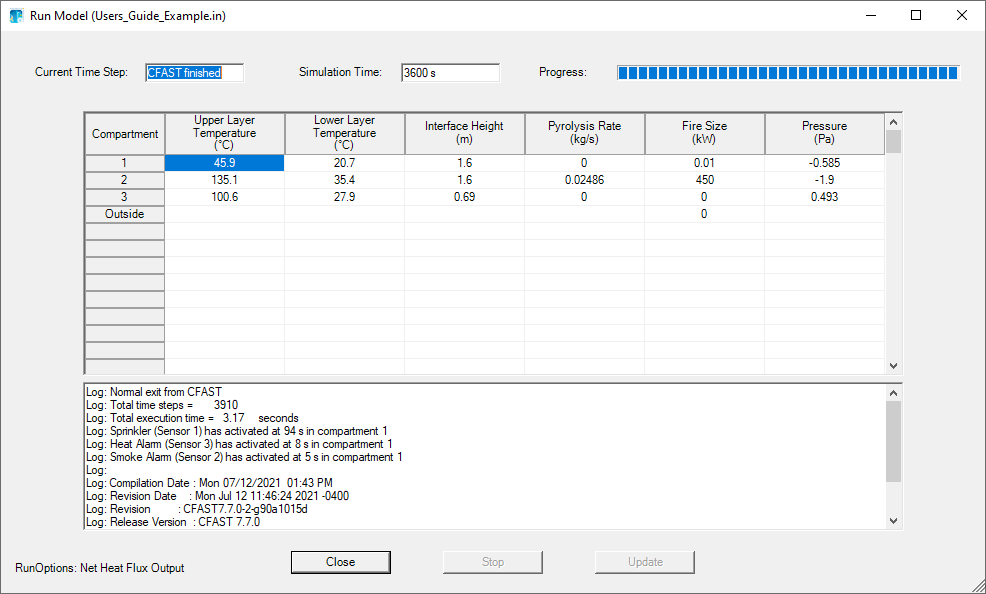
\includegraphics[width=6.5in]{FIGURES/Standard_Output}
\caption[The Standard CFAST Output Screen]{The Standard CFAST Output Screen.}
\label{Run_Model}
\end{figure}


\section{Basic Features}

The input parameters are organized via tabs near the top of the CEdit window, as shown in Fig.~\ref{primary_screen}. The tabs are:
\begin{description}
\item[Simulation Environment] includes simulation time, specification of model outputs, and ambient conditions. Also included on the page is a constantly updated list of errors, warnings, and messages about the input file specification or model simulation.
\item[Thermal Properties] defines the thermal conductivity, specific heat, density, thickness and emissivity values for all materials and fuel sources used in a simulation.
\item[Compartments] defines the size, construction characteristics, and position of the compartments in a simulation.
\item[Wall Vents] define doors and windows.
\item[Ceiling/Floor Vents] define holes in the ceiling/floor.
\item[Mechanical Ventilation] defines forced air ventilation.
\item[Fires] include user specification of the initial fire source and any additional burning objects in one or more of the compartments of the simulation.
\item[Targets] provide the ability to calculate the temperature and net heat flux to objects placed and oriented arbitrarily in the structure.
\item[Detection / Suppression] defines any heat or smoke alarms and sprinklers in the compartments of the simulation.
\item[Surface Connections] allows for more detailed description of the connections between compartments in the simulation to better simulate the transfer of heat from compartment to compartment in the simulation.
\item[Visualizations] allows specification of one or more 2-D and 3-D visualizations to be added to the simulation for viewing with Smokeview. Note that these can require significant additional computational time than a basic CFAST simulation without visualizations.
\end{description}


\section{The View Menu}

The View menu allows you to view or print the input data file, output file (if the simulation has been run and a text output file generated) and the log file of the simulation. If one of the items does not exist on the user's hard disk, the selection is grayed out.
\begin{description}
\item[Select Engineering Units] allows you to select the units for input and output. By default, most outputs are in S.I. units, with temperature in Celsius.
\end{description}


\section{The Help Menu}

The Help menu accesses this user's guide, the CFAST web site, or an about dialog box that displays the user license and version of the program.





\chapter{Simulation Environment}

The Environment page defines the initial conditions and simulation time for the CFAST input file.

\begin{figure}[ht]
\centering
\includegraphics[width=6.5in]{FIGURES/Input_File/Environment_Tab}
\end{figure}

\section{Title}

The first thing to do when setting up an input file is to give the simulation a title. The title is optional and may consist of letters, numbers, and/or symbols and may be up to 50 characters. All output files will be tagged with this character string.


\section{Simulation Times}

\begin{description}
\item[Simulation Time] (default units: s, default value, 900 s): The length of time over which the simulation takes place. The maximum value for this input is 86400 s (1 day).

\item[Text Output Interval] (default units: s, default value, 50 s): The time interval between each printing of the output data.  If omitted or less than or equal to zero, no output values will appear.

\item[Spreadsheet Output Interval] (default units: s, default value, 10 s): CFAST can output the results of the simulation in a comma-delimited spreadsheet file. This parameter defines the time interval between these outputs. A value greater than zero must be used if the spreadsheet file is desired.

\item[Smokeview Output Interval] (default units: s, default value: 10 s): CFAST can output a subset of the results in a format compatible with the visualization program Smokeview. This input defines the time interval between outputs of the model results in a Smokeview-compatible format.  A value greater than zero must be used if the spreadsheet output is desired.

\item[Maximum Time Step] (default units: s, default value: 2 s): CFAST will automatically adjust the time interval for the solution of the differential equation set up or down so that the simulation is as efficient as possible within the pre-defined error tolerances. This parameter places a maximum value for the equation solver and can normally be left at the default value. In cases (which are hopefully rare) where the model fails to converge on a solution, this value can be reduced which often will allow the simulation to successfully complete.
\end{description}

\section{Ambient Conditions}

Ambient conditions define the environment at which the scenario begins. Initial pressures in a structure are calculated simply as a lapse rate (related to the height above sea level) based on the NOAA/NASA tables \cite{GPO:Atmosphere}. It is convenient to choose the base of a structure to be at zero height and then reference the height of the structure with respect to that height.  The temperature and pressure must then be measured at that position.  Another possible choice would be the pressure and temperature at sea level, with the structure elevations then given with respect to mean sea level.  This is also acceptable, but somewhat more tedious in specifying the construction of a structure.  Either of these choices works though, so long as they are consistent. Usually, the station elevation is set to zero and the pressure to ambient. The effect of changing these values is minor. Note that the equations implemented in the model are not designed to handle negative elevations and altitudes.

\begin{description}
\item[Temperature] (default units: \degc, default value: 20 \degc): Initial ambient temperature inside or outside the structure at the station elevation.

\item[Pressure] (default units: Pa, default value: 101300 Pa): Initial values for ambient atmospheric pressure inside and outside the structure at the station elevation. The default value is standard atmospheric pressure at sea level.

\item[Elevation] (defaults units: m, default value: 0 m): The height where the ambient pressure and temperature are specified.  This is the reference height for calculating the density of the atmosphere as well as the temperature and pressure inside and outside of the structure as a function of height.

\item[Humidity] (default units \% RH, default value: 50 \%): The initial relative humidity in the system, only specified for the interior.  This is converted to kilograms of water per cubic meter as an initial condition for both the interior and exterior of the structure.
\end{description}






\chapter{Compartments}

\begin{figure}[h!]
\begin{center}
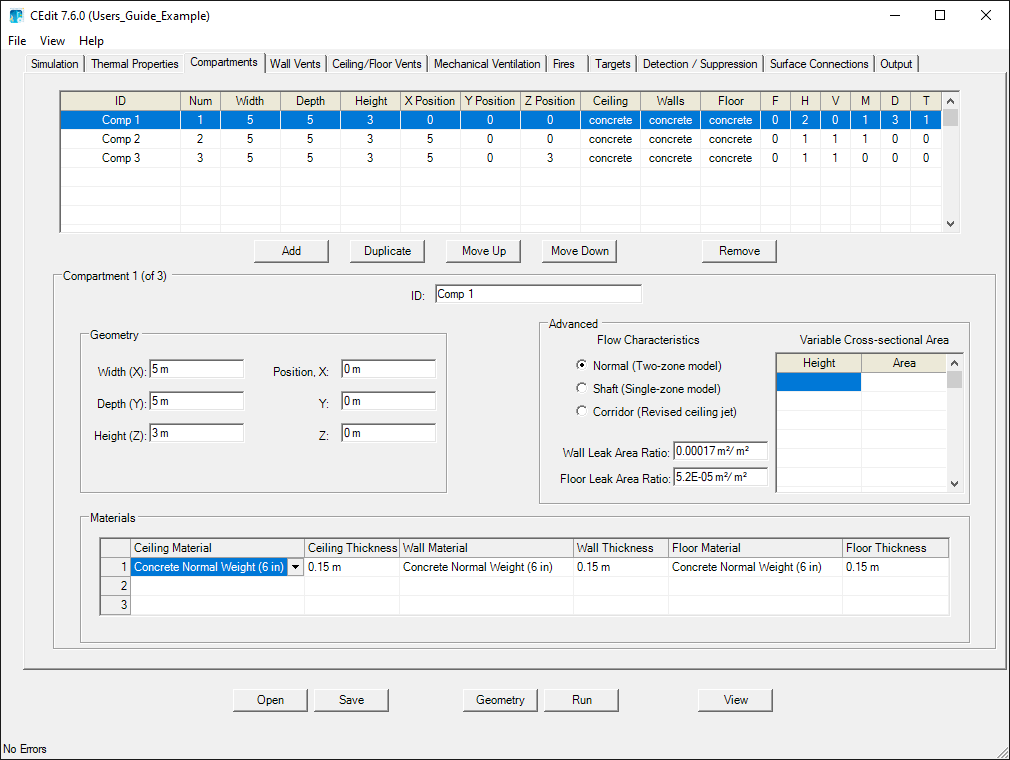
\includegraphics[width=6.5in]{FIGURES/Input_File/Compartment_Geometry_Tab}
\end{center}
\end{figure}

The Compartments page defines the size, position, materials of construction, and flow characteristics for the compartments in the simulation. Initially, only the simulation environment page and the 'Add' button on the compartment geometry page is enabled; all other pages are not available to the user for detailed inputs until a compartment has been added to the simulation.

In order to model a fire scenario, the size and position of each compartment in the structure must be specified. For a compartment, the width, depth, compartment height and height of the floor of the compartment provide this specification. The maximum number of compartments for version 6 is thirty. The usual assumption is that compartments are rectangular parallelepipeds. However, the CFAST model can accommodate odd shapes as equivalent floor area parallelepipeds or with a cross-sectional area that varies with height.

\begin{figure}[h!]
\begin{tabular*}{\textwidth}{c@{\extracolsep{\fill}}c}
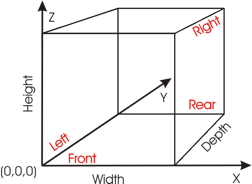
\includegraphics[width=2.5in]{FIGURES/Input_File/CFAST_Coordinates} &
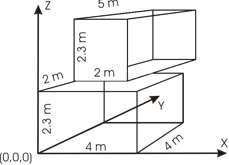
\includegraphics[width=2.6in]{FIGURES/Input_File/CFAST_Absolute_Positioning} \\
Compartment Size & Compartment Position
\end{tabular*}
\end{figure}

At least one compartment must be specified in the input file.  There are no defaults for compartment size. There are defaults for absolute positioning (0,0,0). The fully mixed (single zone) and corridor models are turned off by default.

\label{Compartment_Geometry}Compartments in CFAST are most typically defined by a width, depth, and height.  If desired, compartments can be prescribed by the cross-sectional area of the compartment as a function of height from floor to ceiling for other shapes. The absolute position of the compartment with respect to a single structure reference point can be defined to ease visualization or to allow exact placement of vents and surfaces relative to other compartments in a detailed calculation. This specification is important for positioning the compartments for visualization in Smokeview.

\begin{description}
\item[Compartment Name:] Compartments are identified by a unique alphanumeric name.  This may be a simple as a single character or number, or a description of the compartment.
\end{description}

\section{Geometry}

\label{Compartment_Inputs}
\begin{description}
\item[Width] specifies the width of the compartment as measured on the X axis from the origin (0,0,0) of the compartment.

\item[Depth] specifies the depth of the compartment as measured on the Y axis from the origin (0,0,0) of the compartment.

\item[Height] specifies the height of the compartment as measured on the Z axis from the origin (0,0,0) of the compartment.

\item[Absolute Width Position (Position X)] specifies the absolute x coordinate of the lower, left, front corner of the room.

\item[Absolute Depth Position (Position Y)] specifies the absolute y coordinate of the lower, left, front corner of the room.

\item[Absolute Floor Height (Position Z)] specifies the height of the floor of each compartment with respect to station elevation specified by the internal ambient conditions reference height parameter.  The reference point must be the same for all elevations in the input data.  For example, the two rooms in the sample to the right would be located at (0,0,0) and (0,2,2.3).
\end{description}

\section{Materials}

To calculate heat loss through the ceiling, walls, and floor of a compartment, the properties of the bounding surfaces must be known. This includes the thermophysical properties of the surfaces and the arrangement of adjacent compartments if inter-compartment heat transfer is to be calculated.

The bounding surfaces are the ceilings, walls and floors that define a compartment. These are referred to as thermophysical boundaries, since each participates in conduction and radiation as well as defining the compartments, unless these phenomena are explicitly turned off.

The thermophysical properties of the surfaces which define compartments are described by specifying the thermal conductivity, specific heat, emissivity, density, and thickness of the enclosing surfaces for each material and then assigning the material to the ceiling, walls, and floor of a compartment.  Thermal properties for materials are read from the CFAST input file.  The thermophysical properties are specified at one condition of temperature, humidity, etc.  In CFAST version 6, there can only a single layer per boundary (previous versions allowed up to three).

\begin{description}
\item[Ceiling Material] (default value: Gypsum Board): material name from the thermal properties data file used for the ceiling surface of the compartment.

\item[Wall Material] (default value: Gypsum Board): material name from the thermal properties data file used for the wall surfaces of the compartment.

\item[Floor Material] (default value: Off): material name from the thermal properties data file used for the floor surface of the compartment.
    \end{description}

\graybox{
If the thermophysical properties of the enclosing surfaces are not included, CFAST will treat them as adiabatic (no heat transfer). \\

If a name is used which is not in the input file, the model should stop with an error message. \\

The back surfaces of compartments are assumed to be exposed to ambient conditions unless specifically specified (see the section on Surface Connections) to specify heat transfer connections between compartments).
}

\section{Adding and Editing Thermal Properties}

By default, CEdit does not include predefined thermal properties for compartment materials. Thus, the user needs to define materials for use with a specific simulation.  These may be from other simulations or input directly from reference sources or test results. The \textbf{Edit, Thermal Properties, Insert Thermal Properties} Menu item allows you to add thermal properties from an existing data file to the current simulation.

\begin{figure}[h!]
\begin{center}
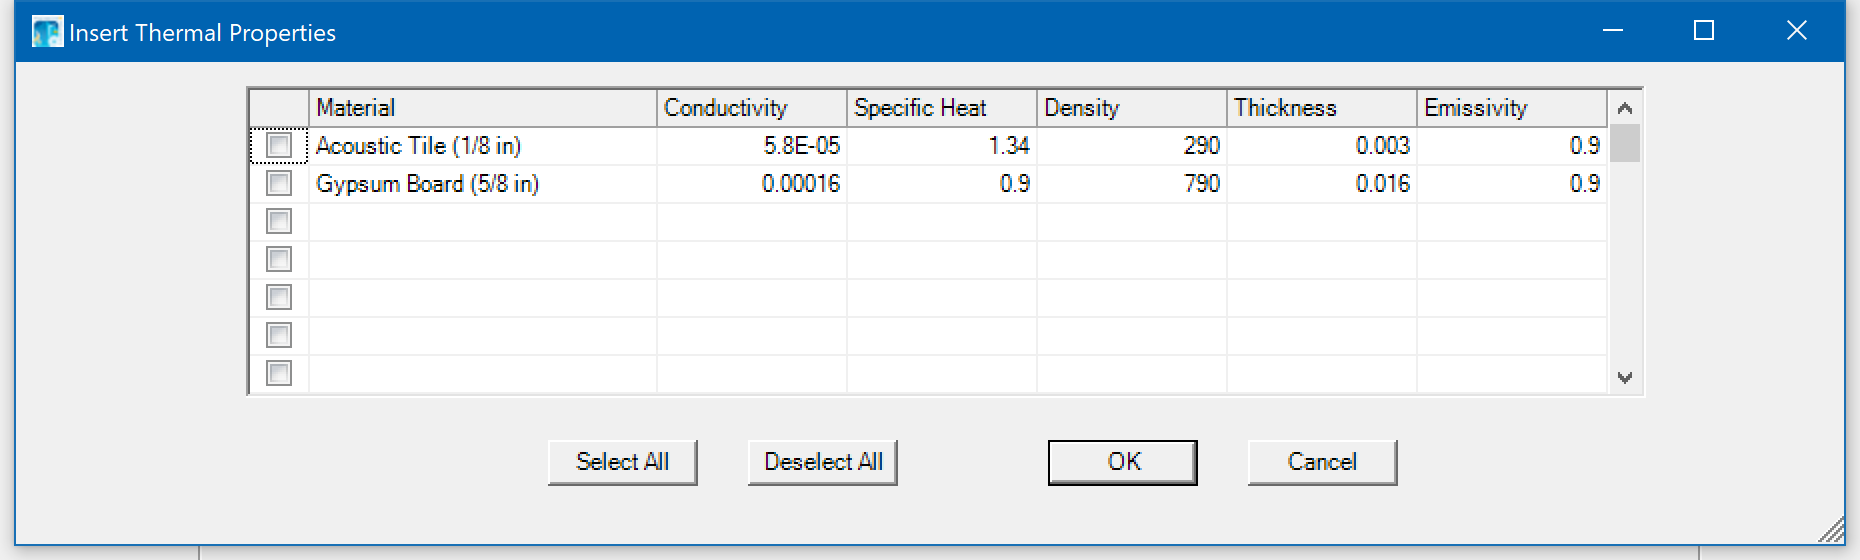
\includegraphics[width=6.5in]{FIGURES/Input_File/Insert_Thermal_Properties}
\end{center}
\end{figure}

To add additional thermal properties to a simulation or to edit existing ones, the \textbf{Edit, Thermal Properties, Edit Thermal Properties} menu item allows you to edit any of the existing thermal properties. \\~ \\

\begin{figure}[h!]
\begin{center}
\includegraphics[width=6.5in]{FIGURES/Input_File/Edit_Thermal_Properties}
\end{center}
\end{figure}

\begin{description}
\item[Material] A descriptive name for the material.

\item[Short Name] A one-word (no more than 8 characters) \textbf{unique} identifier for the material.  This identifier should not contain any spaces and is used in other CFAST inputs to identify the particular material referenced.

\item[Thermal Conductivity] (default value: none, default units: kW/m \degc): Thermal conductivity for the material.

\item[Specific Heat] (default value: none, default units: kJ/kg \degc): Specific heat for the material.

\item[Density] (default value: none, default units: kg/m$^3$): Density for the material.

\item[Thickness] (default value: none, default units: m): Thickness of the material.  Note that if two materials with identical thermal properties but with different thicknesses aer desired, two separate materials must be defined.

\item[Emissivity] (default value: 0.9, default units: none): Emissivity of the material surface.  This is the fraction of radiation that is absorbed by the material.
\end{description}


\section{Modeling a Compartment as a Tall Shaft or Long Corridor}

For tall compartments or those removed from the room of fire origin, the compartment may be modeled as a single, well-mixed zone rather than the default two-zone assumption. A single zone approximation is appropriate for smoke flow far from a fire source, where the two-zone layer stratification is less pronounced than in compartments near the fire or in situations where the stratification does not occur. Examples are elevators, shafts, complex stairwells, or compartments far from the fire.

By specifying the compartment as a corridor, the ceiling jet temperature is calculated with a different empirical correlation that results in a somewhat higher temperature near the ceiling.  This will impact, for example, detectors, sprinkler, and targets near the ceiling in corridors.

\begin{description}
\item[Normal (Two-zone model)] Conditions in the compartment are calculated with the normal two-zone approach.

\item[Shaft (Single-zone model] Conditions in the compartment are calculated as single well-mixed zone.

\item[Corridor (Revised ceiling jet] Conditions in the compartment are calculated with the normal two-zone approach. Ceiling jet temperatures in the compartment are calculated with a revised empirical correlation specific to corridors.
\end{description}


\section{Defining Variable Compartment Area}

The Compartment Geometry page includes two additional entries that may be used for defining compartment properties for spaces which are not rectangular in area.  Values for a chosen compartment are entered in a spreadsheet.

\begin{description}
\item[Height Value(s)] (default units: m, default values: none): Values of height for the corresponding cross-sectional area values measured from the floor of the compartment. The values for the compartment correspond to cross-sectional area values included for the same compartment on the ROOMA command.

\item[Area Value(s)] (default units m$^2$, default values: none): Values of cross-sectional area of the compartment as a function of height measured from the floor of the compartment. The values for the compartment correspond to height values included for the same compartment on the ROOMH command.
\end{description}

\graybox{
Cross-sectional area values may vary larger or smaller with height as appropriate. \\

Overall compartment size (input with the COMPA command (see page \pageref{Compartment_Inputs}) must define a volume at least as large as the total volume of the compartment. Typically, the COMPA input can correspond to the largest area in the list of cross-sectional area values. \\

Once the total compartment volume is determined from the set of cross-sectional area and height inputs, an effective width and depth are calculated (maintaining the original user input for compartment height) so the compartment volume matches to actual total volume of the compartment. The aspect ratio (width/depth)is maintained. \\

Cross-sectional area values should be input in order by ascending height. If the first height value is not zero (i.e., at floor level), the cross-sectional area is assumed constant from the floor to the height specified in the first cross-sectional area value. \\

Similarly, if the last height value is not at the ceiling height, the cross-sectional area is assumed constant from the height specified in the last cross-sectional area value to the ceiling.
Between any two adjacent cross-sectional area data values in the input list, the area is assumed to be a pyramidal section (which by definition maintains the same width to depth aspect ratio for the compartment from floor to ceiling). \\

CFAST uses the variable cross-sectional area inputs to determine the layer height. The equations solved by CFAST determine the volume of the upper layer. For a normal rectangular room, this corresponds directly to a layer height. For a variable cross-sectional area compartment, a  numerical integration of the area inputs beginning at the ceiling is used to determine the height at which the upper layer occupies the calculated volume of the upper layer.
}



\chapter{Natural Ventilation}

Natural ventilation can occur when two compartments are connected via open doorways or windows (\textbf{Wall Vents}); or when two compartments are connected via \textbf{Floor/Ceiling Vents}. If no vents are specified between two compartments, they are assumed to be isolated.

\section{Wall Vents}

\begin{figure}[h!]
\begin{center}
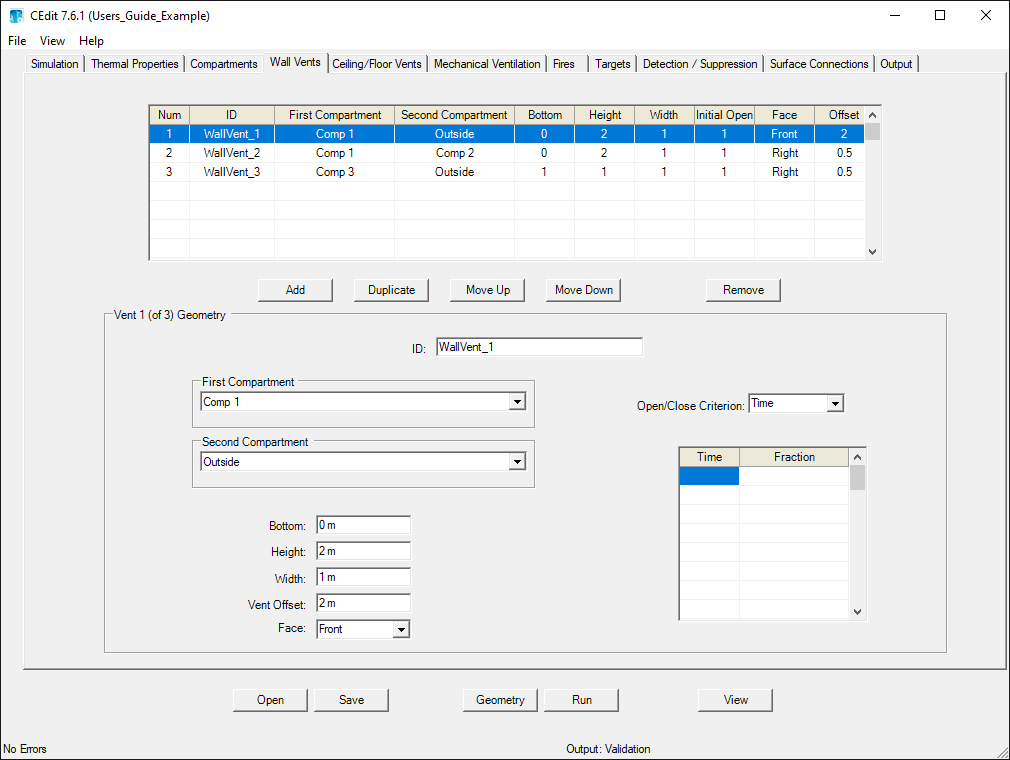
\includegraphics[width=6.5in]{FIGURES/Input_File/Natural_Flow_Tab}
\end{center}
\end{figure}

Wall vents can only be created between compartments that physically overlap in elevation at some point. These may include doors between compartments or windows in the compartments (between compartments or to the outdoors).  Openings to the outside are included as openings to a compartment with a number one greater than the number of compartments described in the geometry section. It is possible to define a total of 25 horizontal flow connections between any pair of compartments. Horizontal flow connections may also be used to account for leakage between compartments or to the outdoors.

\begin{description}
\item[First Compartment] First of the two compartments to be connected by a horizontal flow vent.  Compartments are numbered automatically by the input editor and by the model in the order they are read from the input data file and/or the order they appear in the summary table on the compartment geometry page. Compartment numbers begin with 1, so the first compartment is number 1, the second 2, and so forth.

\item[Second Compartment] Second of the two compartments to be connected by a horizontal flow vent.  Compartments are numbered automatically by the input editor and by the model in the order they are read from the input data file and/or the order they appear in the summary table on the compartment geometry page. Compartment numbers begin with 1, so the first compartment is number 1, the second 2, and so forth.

\item[Sill] (default units: m, default value: none): Sill height is the height of the bottom of the opening relative to the floor of the compartment selected as the first compartment.

\item[Soffit] (default units: m, default value: none): Position of the top of the opening relative to the floor of the compartment selected as the first compartment.

\item[Width] (default units: m, default value: none): The width of the opening.

\item[Initial Opening Fraction] (default value: 1): Flow through horizontal vents is calculated based on the area of the vent.  Normally, the vent is fully open.  If desired, the user may specify a fraction between 0 and 1 that allows the vent to be partially or fully closed at the beginning of the simulation.  In the model calculation, the vent width is multiplied by this fraction.  The opening fraction may be changed at any time in the simulation through the use of the EVENT command.

\item[Change Opening Fraction At Time]  (default units: s, default value: 0 s)  Time during the simulation at which to change the opening fraction.

\item[Final Opening Fraction] (default value: 1): for horizontal flow vents, the fraction specifies the fractional width opening of the vent. Fractional values must be between 0 and 1.

\item[Vent Offset] (default units: m, Default value: 0 m): For visualization, the vent offset is the horizontal distance between the near edge of this vent and the origin of the axis defined by the selected face(below) in the first compartment (Front and Rear are along the X-axis; left and right are along the Y-axis). For example, to place the vent at the center of the front wall, specify the front face at an offset of `compartment width/2 - vent width/2'.

\item[Face] For visualization, FACE specifies which wall the vent will be displayed on in Smokeview.  Choices are Front, Rear, Right, Left and are relative to the X-Z plane.
\end{description}

\graybox{
The soffit and sill specifications are with respect to the first compartment specified and are not necessarily symmetric since the elevation of the second compartment may be different than the first.  Reversing the order of the compartment designations can make a difference.
}

\section{Ceiling/Floor Vents}

\begin{figure}[h!]
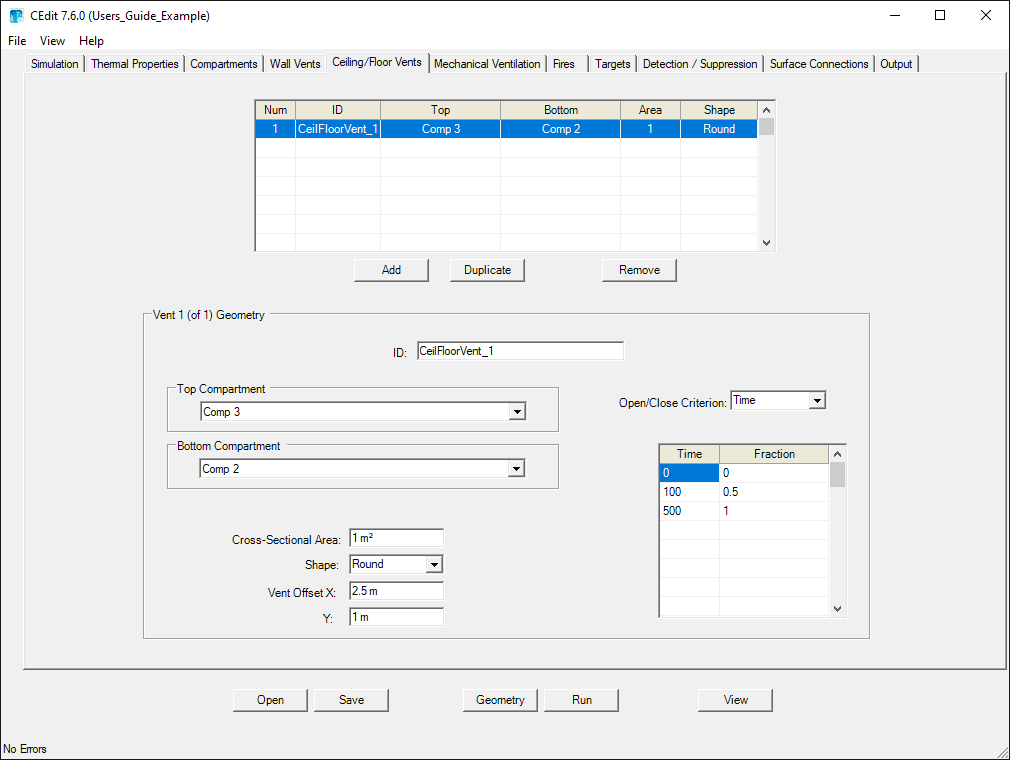
\includegraphics[width=6.5in]{FIGURES/Input_File/Vertical_Flow_Tab}
\end{figure}

This section of the input data file describes the inputs for natural flow vents in ceilings and floors. Examples of these openings are scuddles in a ship, or a hole in the roof of a residence. Combined buoyancy- and pressure-driven flow through a vertical flow vent is possible when the connected spaces adjacent to the vent are filled with gases of different density in an unstable configuration, with the density of the top space larger than that of the bottom space. With a moderate cross-vent pressure difference, the instability leads to a bi-directional flow between the two spaces. For relatively large cross-vent pressure difference the flow through the vent is unidirectional, from the high- to the low-pressure space.

Connections can exist between compartments or between a compartment and the outdoors. Openings to the outside are included as openings to a compartment with a number one greater than the number of compartments defined in the scenario. There are four parameters which include each of the connected compartments, the shape of the opening, and the effective area of the vent.

\begin{description}
\item[Top Compartment] The top or first of the two compartments to be connected by a vertical flow vent. The vent is through the floor of this compartment.  Compartments are numbered automatically by the input editor and by the model in the order that they are read from the input data file and/or the order they appear in the summary table on the compartment geometry page. Compartment numbers begin with 1, so the first compartment is number 1, the second 2, and so forth.

\item[Bottom Compartment] The bottom or second of the two compartments to be connected by a horizontal flow vent. The vent is through the ceiling of this compartment. Compartments are numbered automatically by the input editor and by the model in the order they are read from the input data file and/or the order they appear in the summary table on the compartment geometry page. Compartment numbers begin with 1, so the first compartment is number 1, the second 2, and so forth.

\item[Cross-sectional Area] (default units: m$^2$, default value: none): specifies the cross-sectional area of the vent connecting the two compartments.

\item[Shape] The shape factor is 1 for circular openings and 2 for square openings.

\item[Initial Opening Fraction] Flow through vertical vents is calculated based on the area of the vent.  Normally, the vent is fully open.  If desired, the user may specify a fraction between 0 and 1 that allows the vent to be partially or fully closed at the beginning of the simulation.  In the model calculation, the vent area is multiplied by this fraction.  The opening fraction may be changed at any time in the simulation through the use of the EVENT command.

\item[Change Opening Fraction At Time] (default units: s, default value: 0 s): Time during the simulation at which to change the opening fraction.

\item[Final Opening Fraction] for vertical flow vents, the fraction specifies the fractional cross-sectional area of the vent. Fractional values must be between 0 and 1.
\end{description}

\graybox{
Although obvious, note that the top or first compartment must be the compartment on top of the bottom or second compartment. \\

CFAST allows only a single connection between any pair of compartments included in a simulation. This limitation is based on the implementation of the vertical flow algorithm in CFAST and on the validation efforts for the original algorithm development  which only studied a single opening between connected compartments. \\

Vertical connections can only be created between compartments that could be physically stacked based on specified floor and ceiling elevations for the compartments.  Some overlap between the absolute floor height of one compartment and the absolute ceiling height of another compartment is allowed.  However, whether the compartments are stacked or overlap somewhat, the ceiling/floor absolute elevations must be within 0.01 m of each other. The check is not done when the connection is to the outside.
}


\chapter{Mechanical Ventilation}

\begin{figure}[h!]
\begin{center}
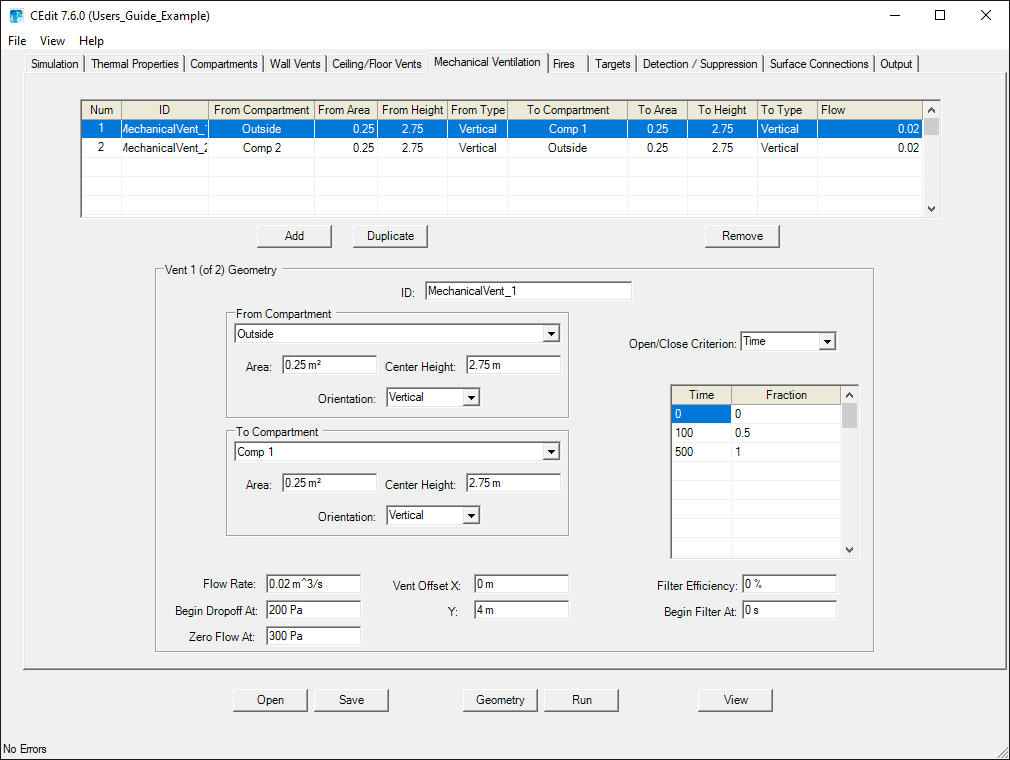
\includegraphics[width=6.5in]{FIGURES/Input_File/Mechanical_Vent_Tab}
\end{center}
\end{figure}

Fan-duct systems are commonly used in buildings for heating, ventilation, air conditioning, pressurization, and exhaust. Generally, systems that maintain comfortable conditions have either one or two fans.  Residences often have a systems with a single fan. Further information about these systems is presented in  Klote and Milke \cite{Klote:2002} and the American Society of Heating, Refrigerating and Air Conditioning Engineers \cite{ASHRAE:2001}.

The model for mechanical ventilation used in CFAST is based on the theory of networks and is based on the model developed by Klote \cite{Klote:1988a}.  This is a simplified form of Kirchoff's law which says that flow into a node must be balanced by flow out of the node. The equations used describe the relationship between the pressure drop across a duct, the resistance of a duct, and the mass flow.  The pressure can be changed by conditions in a compartment, or a fan in line in the duct system.  Resistance arises from the finite size of ducts, roughness on duct surfaces, bends and joints. In CFAST, default values are used for the duct properties, and thus mechanical ventilation connections are simply described by the connections to the two compartments and a fan whose throughput is a constant volumetric flow up to a user-specified pressure drop across the fan, dropping to zero at high backwards pressure on the fan.

\section{Connections to Compartments}

\begin{description}
\item[From Compartment] The first compartment to which the mechanical ventilation system diffuser is connected. Fan flow is from this compartment.  Compartments are numbered automatically by the input editor and by the model in the order they are read from the input data file and/or the order they appear in the summary table on the compartment geometry page. Compartment numbers begin with 1, so the first compartment is number 1, the second 2, and so forth.

\item[From Compartment Area] (default units: m$^2$, default value: none): Cross-sectional area of the opening into the compartment. The area will be truncated if the midpoint (height) is set such that the height plus or minus the effective length is above the compartment ceiling or below the floor.

\item[From Compartment Height] (default units: m, default value: none): Height of the duct opening above the floor of the compartment measured from the midpoint of the register.

\item[From Compartment Orientation] The orientation of the diffuser relative to the floor of the compartment.  A horizontal diffuser implies vertical flow through the ceiling or floor of the compartment.  A vertical diffuser implies horizontal flow through a wall of the compartment.

\item[To Compartment] The bottom or second of the two compartments to be connected by a horizontal flow vent. The vent is through the ceiling of this compartment. Compartments are numbered automatically by the input editor and by the model in the order they are read from the input data file and/or the order they appear in the summary table on the compartment geometry page. Compartment numbers begin with 1, so the first compartment is number 1, the second 2, and so forth.

\item[To Compartment Area] (default units: m$^2$, default value: none): Cross-sectional area of the opening into the compartment. The area will be truncated if the midpoint (height) is set such that the height plus or minus the effective length is above the compartment ceiling or below the floor.

\item[To Compartment Height] (default units: m, default value: none): Height of the duct opening above the floor of the compartment measured from the midpoint of the register.

\item[To Compartment Orientation] The orientation of the diffuser relative to the floor of the compartment.  A horizontal diffuser implies vertical flow through the ceiling or floor of the compartment.  A vertical diffuser implies horizontal flow through a wall of the compartment.
\end{description}

\section{Fans}

\begin{description}
\item[Flow Rate] (default units: m$^3$/s, default value: none): Constant flow rate of the forced-air flow from the first compartment to the second compartment.

\item[Begin Drop Off Pressure] (default units: Pa, default value: 200 Pa): The description of the fan includes a drop off in flow beginning at a pressure specified by the user.  Above this pressure drop, the flow gradually drops to zero flow.

\item[Zero Flow Pressure] (default units: Pa, default value: 300 Pa): Specifies the pressure above which the flow through the mechanical ventilation connection is zero.

\item[Initial Opening Fraction] Flow through mechanical vents is calculated based on the area of the vent.  Normally, the vent is fully open.  If desired, the user may specify a fraction between 0 and 1 that allows the vent to be partially or fully closed at the beginning of the simulation.  In the model calculation, the fan flow rate is multiplied by this fraction.  The opening fraction may be changed at any time in the simulation through the use of the EVENT command.

\item[Change Opening Fraction At Time] (default units: s, default value: none): Time during the simulation at which to change the opening fraction.

\item[Final Opening Fraction] for mechanical flow vents, the fraction specifies the fractional fan flow rate for the vent. Fractional values must be between 0 and 1.
\end{description}

\graybox{
CFAST does not include provisions for reverse flow through a fan. Calibration for backward flow is not provided by fan manufacturers, so the equations incorporated in CFAST do not allow for such flow. The problem is simply that in this flow regime, the fan has stalled, and likely will soon fail. \\

If the simulation includes mechanical ventilation filtering, care should be taken in choosing trace species production rates to insure the production rate is small compared to the total pyrolysis rate.  This will allow appropriate conservation of mass in the solution of the system of differential equation.  For large production rates of trace species, scaling factors can be used (e.g., divide by 1000) for the trace species production rate to reduce the relative magnitude compared to the pyrolysis rate.  For analysis, the resulting trace species in compartments and filters can be converted back to original units multiplying by the scaling factor used.
}

\section{Filtering}

For mechanical vents, there are two species that can be filtered out of the gas flow: soot and the user-defined trace species. Filters are applied only to fan openings. The fan must have been defined before the filter can be applied. Initially filtering is off. It is turned on with the EVENT key word, defined in the input editor with a Filter Efficiency and Begin Filter At time.

\begin{description}
\item[Filter Efficiency] (default units:~\%, default value: none): Flow through mechanical vents may include filtering that removes a user-specified portion of soot and trace species mass from the flow through the vent.  By default, there is no filtering applied, that is all of the soot and trace species mass in the vent flow is passed through the vent. Within the user interface, this is specified as a filter efficiency of 0~\%.  If desired, the user may specify the fraction of the soot and trace species mass to be removed as a percentage.

\item[Begin Filtering At Time] (default units: s, default value: none): Time during the simulation at which the mechanical vent filtering begins.
\end{description}

\graybox{
If the simulation includes mechanical ventilation filtering, care should be taken in choosing trace species production rates to insure the production rate is small compared to the total pyrolysis rate.  This will allow appropriate conservation of mass in the solution of the system of differential equation.  For large production rates of trace species, scaling factors can be used (e.g., divide by 1000) for the trace species production rate to reduce the relative magnitude compared to the pyrolysis rate.  For analysis, the resulting trace species in compartments and filters can be converted back to original units multiplying by the scaling factor used.
}



\chapter{Fires}

A simulated fire in CFAST is implemented as a source of fuel mass which is released at a prescribed rate (the pyrolysis rate). Energy is released by the fuel and combustion products are created as it burns. In the fire, species production is calculated based on production yields prescribed by the user. In addition, the pyrolysis rate and resulting energy and species generation may be limited by the oxygen available for combustion. When sufficient oxygen is available for combustion, the heat release rate for the constrained fire is the same as for the unconstrained fire.

The model can simulate multiple fires in one or more compartments of the building.  These fires are treated as totally separate entities, with no interaction of the plumes. These fires are generally referred to as “objects” and can be ignited at a prescribed time, temperature or heat flux.

CFAST does not include a pyrolysis model to predict fire growth. Rather, pyrolysis rates for each fire are prescribed by the user.  While this approach does not directly account for increased pyrolysis due to radiative feedback from the flame or compartment, in theory these effects could be prescribed by the user as described in this section.  In an actual fire, this is an important consideration, and the specification used should consider the experimental conditions as closely as possible.

A fire releases energy based on the pyrolysis of fuel, but may be constrained by the oxygen available for combustion depending on the compartment conditions. Complete burning will take place only where there is sufficient oxygen.  When insufficient oxygen is entrained into the fire plume, unburned fuel will be transported from zone to zone until there is sufficient oxygen and a high enough temperature to support combustion.  In general, CFAST uses a simple definition of a combustion reaction that includes major products of combustion for hydrocarbon fuels:

\begin{eqnarray}
   \mathrm{C_{n_\C}H_{n_H}O_{n_O}N_{n_N}Cl_{n_{Cl}}} &+&  \nu_\OTWO \, \mathrm{O_2}  \rightarrow  \nonumber \\[.1in]
   \nu_\COTWO \, \mathrm{CO_2} &+& \nu_\HTWOO \, \mathrm{H_2O} \; + \; \nu_\CO \, \mathrm{CO} \; + \; \nu_\So \, \mathrm{Soot} \; + \; \nu_\HCl \mathrm{HCl} \; + \; \nu_\HCN \mathrm{HCN} \label{stoich}
\end{eqnarray} \\
assuming that all the nitrogen and chlorine in the fuel are converted to HCN and HCl. The stoichiometric coefficients $\nu_\So$, $\nu_\CO$, etc. represent appropriate molar ratios for a stoichiometric balance of the equation. For complete combustion of the simplest hydrocarbon fuel, methane reacts with oxygen to form carbon dioxide and water. The only inputs required are the fuel composition, heat release rate, and heat of combustion. For fuels that contain oxygen, nitrogen, or chlorine, the reaction becomes more complex. Stoichiometry is used to insure conservation of mass and elements in the reaction. The species which are calculated are oxygen, carbon dioxide, carbon monoxide, water, total unburned fuel (tuhc), and soot. Gaseous nitrogen is included, but only acts as a diluent.

\begin{figure}[h!]
\begin{center}
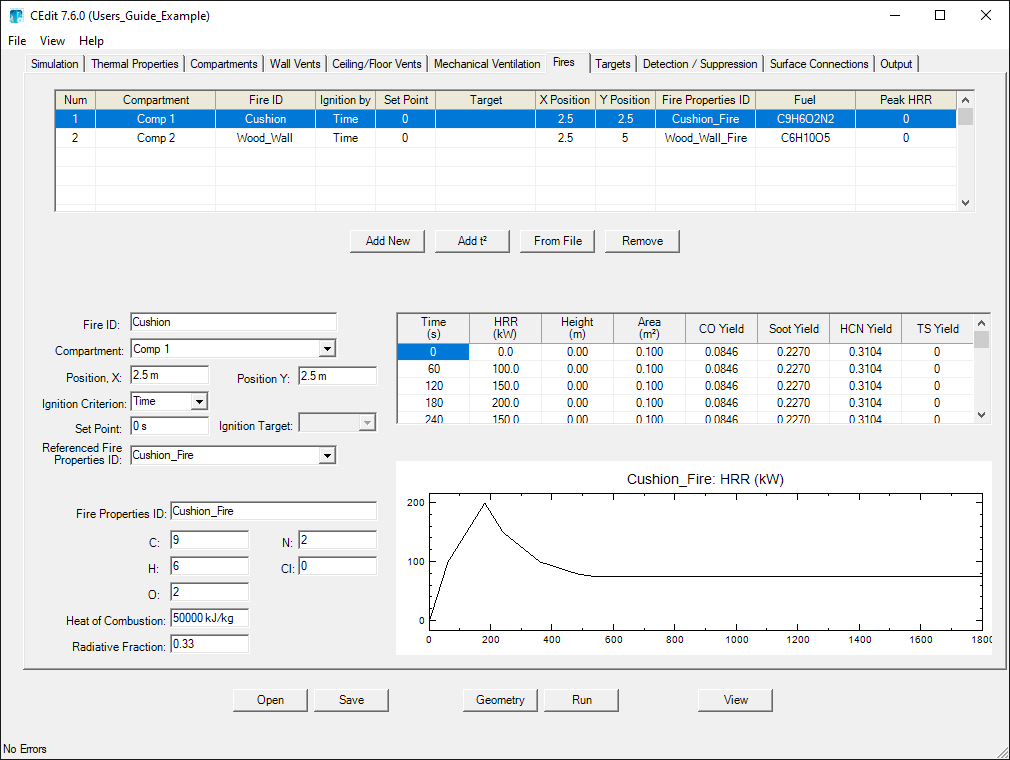
\includegraphics[width=6.5in]{FIGURES/Input_File/Fire_Tab}
\end{center}
\end{figure}

Two inputs on the Fire Tab are global, that is, they apply to all fires included in a simulation.
\begin{description}
\item[Lower Oxygen Limit] (default units: \%, default value: 10~\%):  In the CFAST model, a limit is incorporated by limiting the burning rate as the oxygen level decreases until a ``lower oxygen limit'' (LOL) is reached. The lower oxygen limit is incorporated through a smooth decrease in the burning rate near the limit. Normally, this value would not be changed by the user.

\item[Gaseous Ignition Temperature] (default units: \degc, default value: ambient temperature plus 100 K): The lower temperature limit on the burning of fuel in a gas layer. Since CFAST does not support a combustion kinetics model, this is the algorithm used for fires out of vents.  Normally, this value would not be changed by the user.
\end{description}

\section{Defining Individual Fires}

Fires in CFAST are defined as a series of individual fire objects which are then placed as desired in compartments in a simulation.

Each fire object defines the time dependent variables of the fire described by the mass loss rate, rate of heat release, fuel height, and fuel area.  Species production rates are specified in a manner similar to the fire, entering the rates as a series of points with respect to time.  The species which are followed by CFAST are: carbon dioxide, carbon monoxide, hydrogen cyanide, hydrogen chloride, nitrogen, oxygen, soot, total unburned hydrocarbons and water. There is a separate calculation of the concentration-time product Ct. Finally, a user-specified trace species can be specified to follow the transport that results from fire-induced flow for an arbitrary species. This may be of particular interest for radiological releases \cite{Jones:2008}, but may be useful for any trace amounts released by a fire.

Each fire object is defined in a separate comma-separated spreadsheet file with an extension of ``.o'' and is also saved in the CFAST input file for the current simulation. A pull-down allows the user to select one of the predefined fire objects to place in the chosen compartment. As many fire objects as desired may be defined by the user.  At least one fire in the simulation should ignite at a user-specified time.  Other fire objects can ignite based on time, temperature or heat flux conditions.

\begin{figure}[h!]
\begin{center}
\includegraphics[width=6.5in]{FIGURES/Input_File/Fire_Object_Edit}
\end{center}
\end{figure}

\begin{description}
\item[Fire Object Name] The name for the desired object.  This also corresponds to the name of the fire object file, without the extension. The selected name must be unique (i.e., not the same as another fire object in the same simulation).

\item[Material] (default value: none): material name from the list of thermal properties used for the object. The material properties are used to calculate heat transfer into the object from its surroundings.

\item[C, H, O, N, Cl] Molecular formula of the burning fuel. Burning fuels in CFAST are assumed to be hydrocarbon fuels that contain at least Carbon and Hydrogen and optionally Oxygen, Nitrogen, and Chlorine. These five inputs define the stoichiometry of the fuel as it is burned.  Thus, for example, all of the specified Nitrogen and Chlorine is assumed to completely react to form HCN and HCl.  If only partial conversion is desired, a smaller ratio for Nitrogen and/or Chlorine can be specified.

\item[Heat of Combustion] (default units: J/kg, default value: 50 000 000 J/kg): The energy released per kilogram of mass burned.

\item[Soot Yield] (default units: kg/kg, default value: 0 kg/kg): Constant species yields of soot expressed as ratios of carbon to fuel produced by the pyrolysis of the fuel. This input allows the user to specify a single value for soot yield for all time points in the fire time line. Individual time points can be changed as desired in the spreadsheet input described below.

\item[CO Yield] (default units: kg/kg, default value: determined by correlation): Constant species yield of carbon monoxide expressed as a fraction of the fuel mass converted into carbon monoxide.  By default, the CO yield is related to the soot yield via the correlation developed by K\"oyl\"u and Faeth

\be
y_{CO} = \frac{12n_C}{M_fv_f}0.0014 + 0.37y_s \label{eq:Koylu}
\ee
where $n_C$ is the number of carbon atoms in a fuel molecule, $M_f$ is the molecular weight of the fuel, and $v_f$ is the stoichiometric coefficient of the fuel, assumed to be 1 here \cite{Koylu:1991}. Note that this correlation refers to well-ventilated fires. Yields of CO and soot in under-ventilated fires is still a subject of active research.

\item[Radiative Fraction] The fraction of the energy produced in combustion that is radiated from the fire and plume. Within CFAST, the radiative fraction defaults to 0.35 ; i.e., 35 \% of the fire’s energy is released via radiation.  For other fuels, the work of Tewarson \cite{Tewarson:2003}, McCaffrey \cite{McCaffrey:1982}, or Koseki \cite{Koseki:1989} is available for reference.  The typical range for the radiative fraction is from about 0.05 to 0.4.
\end{description}

For all fires, including t-squared fires, values are calculated for time dependent variables, including default values for species generation. For all inputs, these values can be changed. All of the time dependent variables depend on a predefined time line. The time input specifies a sequence of time points that define the timing of the fire.  An entry indicates a point on the time-line when the mass loss rate, fuel height and other time dependent values are specified for the fire.  This time is independent of the simulation time which is specified by the TIMES line. If the simulation time is longer than the total duration of the fire, the final values specified for the fire (mass loss rate, fuel height, fuel area, and species) are continued until the end of the simulation.

\begin{description}
\item[Time] (default units: s, default values: none): specify a sequence of time points that define the timing of the main fire.  An entry indicates a point on the time-line when the heat release loss rate, fuel height and other time dependent values are specified for the fire.

\item[Heat Release Rate (Qdot)] (default units: kW, default values: none): Heat release rate of the fire as a series of time points consistent with the time specification.

\item[Fire Height] (default units: m, default values: 0 m): Time-based values for height of the base of the fire.  Actual height of the base of the fire is the sum of the constant value specified for the fire and this height specification for a particular time in the fire development.

\item[Area] of the Base of the Fire (default units: m$^2$, default values: 0.3 m$^2$): Cross-sectional area of the base of the fire.

\item[CO Yield] (default units: kg/kg, default values: constant value from correlation, in eq. \ref{eq:Koylu}): yield of carbon monoxide expressed as a fraction of the fuel mass converted into carbon monoxide.

\item[Soot Yield] (default units kg/kg, default values: none): yield of soot expressed as a fraction of fuel mass converted into smoke particulate..

\item[Ct] (default units: kg/kg, default values: none): Yield of a fictitious toxic species per mass of fuel produced in the pyrolysis of the fuel.

\item[TS] (default units: kg/kg, default values: none): Yield of user-defined trace species per mass of fuel produced in the pyrolysis of the fuel.
\end{description}

\graybox{

Production of hydrogen cyanide and hydrogen chloride are tracked solely based on user prescribed yields. \\

The heat release rate for a constrained fire may be reduced below its prescribed value based upon the oxygen available for combustion. For the constrained fire, the burning rate may be less than the pyrolysis rate and cannot be simplified as in the case of the unconstrained fire. As fuel and oxygen are consumed, heat is released and various products of combustion are formed. \\

For a constrained fire, the heat release rate is limited by available oxygen. This limit is applied in three places: The first is burning in the portion of the plume which is in the lower layer of the room of fire origin; the second is the portion of the plume in the upper layer, also in the room of origin; the third is in the vent flow which entrains air from a lower layer into an upper layer in an adjacent compartment. The unburned fuel is tracked in this model. Combustion of CO to CO$_2$ is not included in the model. Detailed combustion chemistry is not considered in CFAST due to the complexities associated with detailed kinetics and transport. \\

There are two calculations involving radiation in this model. One is for the overall energy balance and is based on broadband radiation absorption. The amount of radiation absorbed is sensitive to the species present, specifically water vapor, soot and carbon dioxide. The other is for visibility of egress signs. This calculation is based solely on the soot volume fraction and is reported as optical depth (per meter). The conversion factor is based on the recent work by Mulholland and Croarkin \cite{Mullholland:2000}. The value for converting mass density in kg/m3 to optical depth is 3817 m$^2$/kg. The value reported is intended specifically for assessing the visibility of egress signs, based on the work of Jin \cite{Jin:1979}.  It is not applicable to the far blue or red regions of the spectrum and so should not be used for assessing optical detection of fires through smoke. \\

With the two parameters, heat of combustion ($H_C$) and heat release rate $\dQ$, the pyrolysis rate of the fuel is determined by $\dm=\frac{\dQ}{H_C}$. \\

By default, the fire is placed in the center of the compartment on the floor.  If values for any of the three variables are invalid (i.e., less than zero or greater than the compartment dimension in the appropriate direction), the location for that direction defaults to the center of the appropriate direction in the width or depth direction and at the floor for the vertical direction. \\

The area of the base of the fire should not be left at a value of zero. Radiation from the fire is determined by a point source calculation from the vertical center of the flame which is in turned determined by Heskestad's flame height correlation \cite{Heskestad:2002}, a function of heat release rate and fire area. \\

For “normally toxic” materials, Ct takes a value of 1 and is typically changed by an order of magnitude for particularly toxic or non-toxic materials.  It is not part of the mass balance for the fuel and system, but it just carried along as a transported species in flow through the structure. Ct is used as a measure of toxicity of a material.  Typically the integrated Ct versus time product is calculated. For normal materials, a concentration-time product of 900 mg min/m$^3$ is an indication of incapacitation. \\

The trace species is transported along with fire gases, but is assumed not to take part in the combustion reaction and is assumed not to be a significant source of overall mass for the system mass balance calculated by the model. This implies that the production rate of trace species specified should be much smaller than the total specified pyrolysis rate. If necessary, the trace species can be scaled to a smaller value (e.g., divided by 1000) for the simulation and converted back for analysis (e.g., multiplied by 1000). \\

In the input editor, time-dependent data are entered in a simple spreadsheet. Normal windows copy (Ctrl-C), cut (Ctrl-X), and paste (Ctrl-V) keyboard shortcuts are available for data editing. In addition, Alt-Ins will insert a complete row above the currently-selected row in the spreadsheet and Alt-Del will delete the current row in the spreadsheet.
}

\subsection{Adding and Editing Fires}

By default, CEdit does not include predefined fires. Thus, the user needs to define fire objects for use with a specific simulation.  These may be from other simulations or input directly from reference sources or test results. The \textbf{Edit, Fires, Insert Fires} Menu item allows you to add fires from an existing data file to the current simulation.

\begin{figure}[h!]
\begin{center}
\includegraphics[width=6.5in]{FIGURES/Input_File/Insert_Fire_Objects}
\end{center}
\end{figure}

\subsection{T-squared Fires}

Use the Create t$^2$ button to create a new fire object with a heat release rate specified by the user in the form of a t-squared fire.  For a wide range of fires, the fire growth can be accurately represented with a power law relation of the form $\dQ=\alpha t^2$  where $\dQ$  is the heat release rate of the fire, $\alpha$ is the fire intensity coefficient, and $t$ is time \cite{Schifiliti:2002}. A set of specific t-squared fires labeled slow, medium, and fast, with fire intensity coefficients ($\alpha$) such that the fires reached 1054 kW (1000~BTU/s) in 600~s, 300~s, and 150~s, respectively were proposed for design of fire detection systems .  Later, these specific growth curves and a fourth called "Ultra-fast" which reaches 1054~kW in 75~s, gained favor in general fire protection applications. A separate window allows the user to define the t-squared fire. Details of the inputs for a t-squared fire is included below.

\begin{figure}[h!]
\begin{center}
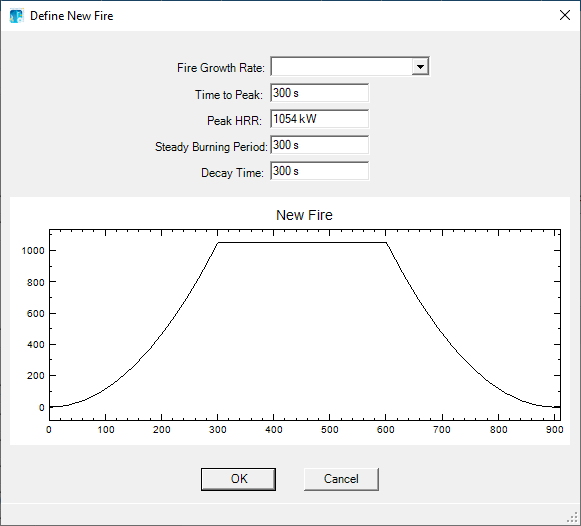
\includegraphics[width=5in]{FIGURES/Input_File/Create_t2}
\end{center}
\end{figure}

\begin{description}
\item[Fire Growth Rate] A set of specific t-squared fires labeled slow, medium, fast, or ultra-fast with fire intensity coefficients ($\alpha$) such that the fires reached 1054~kW (1000~BTU/s) in 600~s, 300~s, 150~s, and 75~s are available.  Each of these growth rates (with corresponding decay rates) can be selected. A fifth, custom, selection allows the user to define any growth or decay rate desired.

\item[Time to Peak] (default units: s, default value: 300 s): The time for the fire to reach the peak fire size.

\item[Peak HRR] (default units: kW, default value: 1054 kW): The peak heat release rate of the t-squared fire.  Fire size is constant beginning at a time consistent with the time to reach the peak value,   and continues at that value for the time specified in the steady burning period, below.

\item[Steady Burning Period] (default units: s, default value: 300 s): Duration of time that the fire continues burning at the rate specified by the maximum HRR input, above.

\item[Decay Period] (default units: s, default value, 300 s): Duration of time for the fire to decay back to a zero value.  Decay follows the inverse of the t-squared growth rate.
\end{description}

\section{Fire Location}

Fires  are placed in defined positions within a compartment of a simulation and oriented with a normal vector to the surface of the object.  Ignition of an object may be at a specified time, a specified net incident heat flux on the surface of the object, or at a specified surface temperature of the object.

\begin{description}
\item[Compartment] of Fire Origin: specifies the compartment that contains the main fire for the simulation.  Any compartment defined is valid.

\item[Position X] (default units: m, default value: compartment width / 2): Position of the center of the base of the fire measured in the x direction from the front lower left corner of the compartment origin (0,0,0) in the compartment of fire origin.

\item[Position Y] (default units: m, default value: compartment depth / 2): Position of the center of the base of the fire measured in the y direction from the front lower left corner of the compartment origin (0,0,0) in the compartment of fire origin.

\item[Position Z] (default units: m, default value: 0 m): Position of the center of the base of the fire measured in the z direction from the front lower left corner of the compartment origin (0,0,0) in the compartment of fire origin. Actual height of the base of the fire is the sum of the value specified by FPOS and by FHIGH for a particular time in the fire development.

\item[Normal  X] Component: specifies a vector of unit length perpendicular to the exposed surface of the object. (Depth) component is in the direction from the rear wall of the object compartment. Default value is a horizontal, upward facing object, unit vector = (0,0,1)

\item[Normal  Y] Component: specifies a vector of unit length perpendicular to the exposed surface of the object. (Breadth) component is in the direction from the left wall of the object compartment. Default value is a horizontal, upward facing object, unit vector = (0,0,1)

\item[Normal  Z] Component: specifies a vector of unit length perpendicular to the exposed surface of the object. (Breadth) component is in the direction from the floor of the object compartment. Default value is a horizontal, upward facing object, unit vector = (0,0,1)

\item[Ignition Criterion] The type of ignition condition specified by the Ignition Criterion Value. Acceptable values are 1 for time, 2 for object surface temperature, and 3 for incident flux to object surface.

\item[Ignition Value] The numerical value at which ignition will occur. If it is less than or equal to zero, the default value of zero is taken.
\end{description}

\section{Calculating Normal Vectors}

The general equations for determining the normal vectors in the x, y, and z directions are \\~

Normal vector in the x direction, $x = \sfrac{x}{\sqrt{x^2 + y^2 + z^2}}$ \\

Normal vector in the y direction, $y = \sfrac{y}{\sqrt{x^2 + y^2 + z^2}}$ \\

Normal vector in the z direction, $z = \sfrac{z}{\sqrt{x^2 + y^2 + z^2}}$ \\

The simplest way to calculate the unit vector is to draw an imaginary line at right angles (i.e., 90$^\circ$ angle) from the exposed surface of the target and to extend this imaginary line until it hits the walls, floor or ceiling of the compartment in which it is located.  This imaginary line is actually a vector that starts at the surface of the exposed target and terminates on a wall, floor, or ceiling.  Once the start point and the end point of a vector are known, the unit vector for this imaginary line may be calculated as follows:

\begin{equation}
  \begin{aligned}
 x &= \sfrac{x_{end} - x_{start}}{\sqrt{\brackets{x_{end} - x_{start}}^2 + \brackets{y_{end} - y_{start}}^2 + {z_{end} - z_{start}}^2}} \\
 y &= \sfrac{y_{end} - y_{start}}{\sqrt{\brackets{x_{end} - x_{start}}^2 + \brackets{y_{end} - y_{start}}^2 + {z_{end} - z_{start}}^2}} \\
 z &= \sfrac{z_{end} - z_{start}}{\sqrt{\brackets{x_{end} - x_{start}}^2 + \brackets{y_{end} - y_{start}}^2 + {z_{end} - z_{start}}^2}}
  \end{aligned}
\end{equation}

As an example, assume the following scenario:

\begin{itemize}
\item A square shaped target object is located in the middle of the floor of a compartment.
\item The target is constructed from non-combustible materials except the top.
\item The square shaped material is 1 m in depth, 1 m in breadth, and 1 m high.
\item The reference point (0,0,0) in the compartment is the lower left hand side of the rear wall.
\item The compartment is 3 meters in the x direction (i.e., the distance from the rear wall to the front wall of the compartment), 4 meters in the y direction (i.e., the distance from the left wall to the right wall of the compartment), and 5 meters in the z direction (i.e., the distance from the floor to the ceiling of the compartment).
\end{itemize}

Since the only side of the target that is combustible is the top surface of the target object, an imaginary line is draw perpendicular (i.e., at a 90$^\circ$ angle) from the top surface of the target object and extended until it reaches the outer boundary of the compartment.  In this case, since the top of the target object is facing the ceiling, the imaginary line would run straight up to the ceiling, running parallel to the four walls of the compartment, and terminating at the ceiling at the point (1.5 m, 2 m, 5 m).  Since the vector starts at point (1.5-m, 2-m, 1-m) and terminates at (1.5-m, 2-m, 5-m), the unit vectors can be calculated as follows:


\begin{equation}
  \begin{aligned}
 x &= \sfrac{x_{end} - x_{start}}{\sqrt{\brackets{x_{end} - x_{start}}^2 + \brackets{y_{end} - y_{start}}^2 + {z_{end} - z_{start}}^2}} &= \sfrac{1.5 - 1.5}{\sqrt{\brackets{1.5 - 1.5}^2 + \brackets{2 - 2}^2 + {5 - 1}^2}} \\
 y &= \sfrac{y_{end} - y_{start}}{\sqrt{\brackets{x_{end} - x_{start}}^2 + \brackets{y_{end} - y_{start}}^2 + {z_{end} - z_{start}}^2}} &= \sfrac{2 - 2}{\sqrt{\brackets{1.5 - 1.5}^2 + \brackets{2 - 2}^2 + {5 - 1}^2}} \\
 z &= \sfrac{z_{end} - z_{start}}{\sqrt{\brackets{x_{end} - x_{start}}^2 + \brackets{y_{end} - y_{start}}^2 + {z_{end} - z_{start}}^2}}  &= \sfrac{5 - 1}{\sqrt{\brackets{1.5 - 1.5}^2 + \brackets{2 - 2}^2 + {5 - 1}^2}} \\
  \end{aligned}
\end{equation}

In this case, the unit vector in the +Z direction.



\chapter{Sprinklers and Detectors}

Sprinklers and detectors are both considered detection devices by the CFAST model and are handled using the same inputs.  Detection is based upon heat transfer to the detector. Fire suppression by a user-specified water spray begins once the associated detection device is activated.

\begin{figure}[h!]
\begin{center}
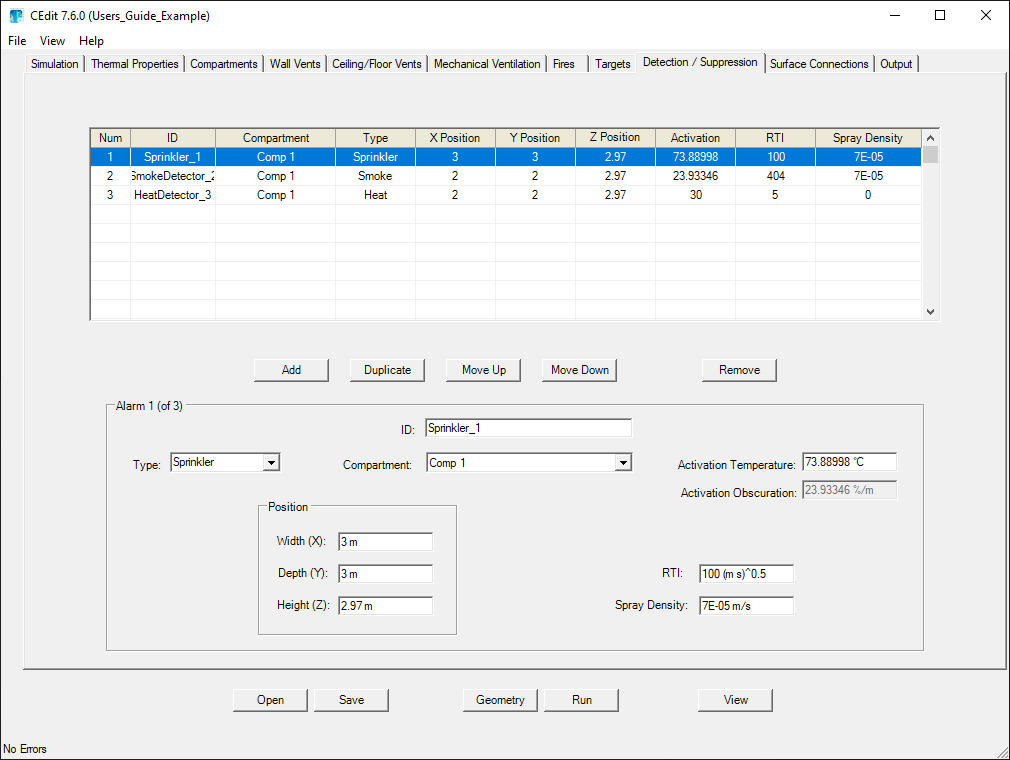
\includegraphics[width=6.5in]{FIGURES/Input_File/Detector_Tab}
\end{center}
\end{figure}

\begin{description}
\item[Type] type of detector, select smoke detector, heat detector, or sprinkler.

\item[Compartment] the compartment in which the detector or sprinkler is located.

\item[Activation Temperature] (default units: \degc, default value: dependent on type): the temperature at or above which the detector link activates.

\item[Width (X)] Position (default units: m, default value: none): position of the object as a distance from the left wall of the compartment (X direction).

\item[Depth (Y)] Position (default units: m, default value: none): position of the detector or sprinkler as a distance from the front wall of the compartment (Y direction).

\item[Height (Z)] Position (default units: m, default value: none): position of the object as a distance from the floor of the compartment (Z direction).

\item[RTI] (default units: (m$\cdot$s)$^{1/2}$, default value: none): the Response Time Index (RTI) for the sprinkler or detection device.

\item[Spray Density] (default units: m/s, default value: none): the amount of water dispersed by a sprinkler.  The units for spray density are length/time, derived by dividing the volumetric flow rate by the spray area. The suppression calculation is based upon an experimental correlation by Evans~\cite{Evans:1993}.
\end{description}

\graybox{
Often, the activation of smoke alarms is simulated with a temperature-based criterion, typically in the range of 5~\degc to 10~\degc above ambient. Davis and Notarianni  studied the activation of heat and smoke alarms in small and large compartments \cite{Davis:1996}. They conclude that a temperature rise of approximately 5~\degc corresponded to activation of ionization alarms for a range of fire sources and ceiling heights. The Nuclear Regulatory Commission includes a default value of 10~\degc in NUREG-1805 \cite{NRCNUREG1805}. \\

Several cautions should be observed when using estimates of sprinkler suppression within the model: 1) the first sprinkler activated controls the effect of the sprinkler on the heat release rate of the fire.  Subsequent sprinklers which may activate have no additional effect on the fire simulation. 2) The fire suppression algorithm assumes the effect of the sprinkler is solely to reduce the heat release rate of the fire. Any effects of the sprinkler spray on gas temperatures or mixing within the compartment are ignored. 3) The sprinkler always reduces the heat release rate of the fire. The ability of a fire to overwhelm an under-designed sprinkler is not modeled. 4) Since the dynamics of the sprinkler and direct effects of the spray on gas temperatures and velocities are not modeled, calculated times of activation of secondary sprinklers and / or detectors after the first sprinkler is activated should be not be modeled since the impact of the first sprinkler on the activation of additional sprinklers is not included in the CFAST model.
}



\chapter{Defining Targets}

CFAST can track and report calculations of the net heat flux striking arbitrarily positioned and oriented targets and the temperature of these targets.

\begin{figure}[h!]
\begin{center}
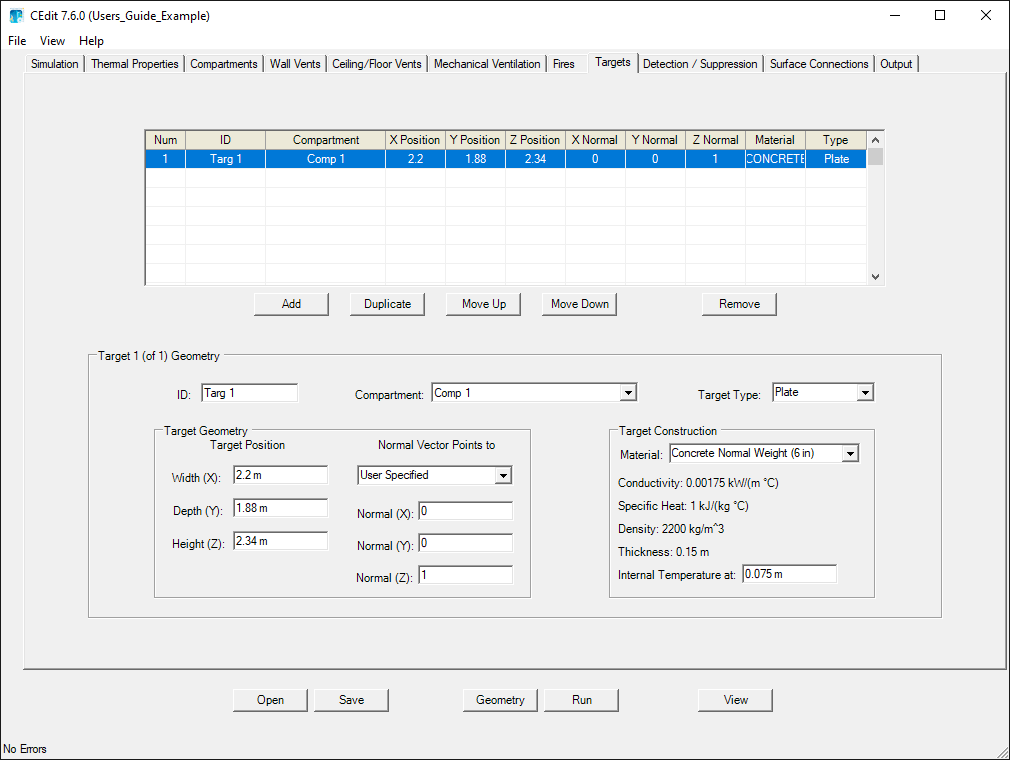
\includegraphics[width=6.5in]{FIGURES/Input_File/Target_Tab}
\end{center}
\end{figure}

In addition to any user-defined targets, there are always two targets that are automatically placed in any compartment containing a fire. Both are included for reporting purposes. The first is an “ambient target” and is intended to represent the net flux to a human body. This is used for the flux in the hazard calculation for tenability. The assumption is that the target will remain at ambient temperature, which is a surrogate for body temperature. The second determines the net flux to a horizontal target on the floor whose temperature is assumed to be the same as the floor surface. The calculation can be used to estimate the ignition of combustibles on the floor as a surrogate for estimating time to flashover, typically taken to be 20 kW/m$^2$. Thus if user-specified targets are included, they will be in addition to these two predefined targets.

For all targets, heat flux is calculated to the surface specified by the user (with the direction determined by the normal vector). Conduction into the target is assumed to occur only from this surface into the target.

\begin{description}
\item[Compartment] The compartment in which the target is located.

\item[Target Type] If the solution method is not STEADY, this parameter further indicates the solutions equations.  Specify Thermally Thick, Thermally Thin, or Cylindrical.  For thermally thin materials, CFAST uses ordinary differential equations; for thermally thick materials, partial differential equations, and for cylindrical targets, cylindrical coordinates.

\item[Solution Method] Optional parameter that indicates the solution method. STEADY for steady state solution, EXPLICIT for explicit solution, IMPLICIT for implicit solution.

\item[Width (X)] Position (default units: m, default value: none): Position of the target as a distance from the left wall of the target compartment (X direction).

\item[Depth (Y)] Position(default units: m, default value: none): Position of the target as a distance from the front wall of the target compartment (Y direction).

\item[Height (Z)] Position(default units: m, default value: none): Height of the target above the floor (Z direction).

\item[Normal Vector X] Component: specifies a vector of unit length perpendicular to the exposed surface of the target. (Width) component in the direction from the left wall of the target compartment. A value of 1 defines a vertical target facing into the compartment, unit vector = (1,0,0). The X, Y, and Z component of the normal vector can also be calculated automatically with a pull down menu that allows selection of surfaces and fires in the compartment visible from the target location.

\item[Normal Vector Y] Component: specifies a vector of unit length perpendicular to the exposed surface of the target. (Depth) component in the direction from the front wall of the target compartment. A value of 1 defines a vertical target facing to the right, unit vector = (0,1,0).

\item[Normal Vector Z] Component: specifies a vector of unit length perpendicular to the exposed surface of the target. (Height) component in the direction from the floor of the target compartment. Default value is a horizontal, upward facing target, unit vector = (0,0,1).

\item[Material] Used to specify the wall material of the target.  Any existing material in the list of thermal properties may be used here.

\item[Internal Temperature at] (default units: none, default value: 0.5): For each target, CFAST calculates the internal temperature at a number of node points within the target. By default, the reported internal temperature (in the printed and spreadsheet output) is the temperature at the center of the target, e.g., equidistant from the front and back faces of the target. This input allows the user to override this default position. The input represents the position as a fraction of the thickness from the front surface to the back surface of the material.
\end{description}

\graybox{
Target inputs in CFAST perform a heat transfer calculation between the compartment and the target. The steady state option assumes that the target material reacts instantly to changing conditions and computes the target temperature that would result in a balance of incoming and outgoing heat (i.e., a steady state). If a transient target temperature is modeled, then one can either assume that there is a temperature variation within the target or assume that the target is “thin” and can be modeled using only one temperature. If the target is assumed to be thin then the ODE option should be used set since this is how the equations are solved. If the target is assumed to be thick then the PDE option should set. Finally, if one of the two transient options are set (ODE or PDE), the numerical solution can be solved using an explicit or an implicit method.  Typically, the implicit method will work in all cases.  The explicit method is recommended only when the implicit method fails to come to a solution.
}



\chapter{Surface Connections}

\begin{figure}[h!]
\begin{center}
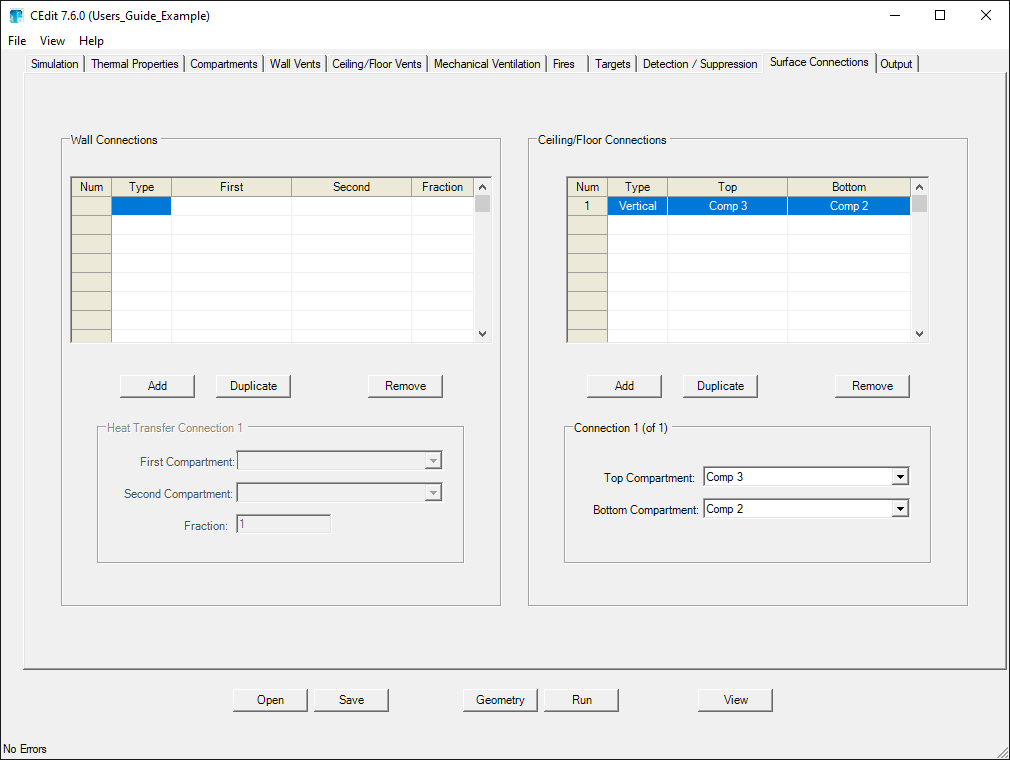
\includegraphics[width=6.5in]{FIGURES/Input_File/Surface_Connection_Tab}
\end{center}
\end{figure}

The Surface Connections page allows the user to define heat transfer between compartments in a simulation. Energy can be transferred from compartment to compartment through solid boundaries (walls, ceilings and floors) by means of conduction. The heat transfer between connected compartments is modeled by merging the connected surfaces for the ceiling and floor compartments or for the connected horizontal compartments.  The heat conduction problem is solved for the merged walls using a temperature boundary condition for both the near and far wall. As before, temperatures are determined by the solver so that the heat flux striking the wall surface (both interior and exterior) is consistent with the temperature gradient at that surface.

\begin{description}
\item[First Compartment] First of the connected compartments. Order of the inputs is not important.

\item[Second Compartment] Second of the connected compartments. Order of the inputs is not important.

\item[Fraction] Specifies the fraction of the vertical surface areas of the compartments which are connected can be specified. The fraction specifies the fraction of the vertical surface area connecting the first and second compartment pair.

\item[Top Compartment] The top or first of the two compartments to be connected by a vertical heat transfer connection. The connection is through the floor of this compartment.

\item[Bottom Compartment] The bottom or second of the two compartments to be connected by a vertical heat transfer connection. The connection is through the ceiling of this compartment.
\end{description}



\chapter{Visualization}

Calculated results from a CFAST simulation can be visualized using Smokeview \cite{Smokeview_Users_Guide_6}. This allows the user to see the compartment geometry and connections or view the results of the simulation visually. In addition to a simplified view of the layer temperatures and vent flows, more detailed estimates of gas temperature, gas velocity, vent flow velocity, target temperature, and detector status can be visualized.

\begin{figure}[h!]
\begin{center}
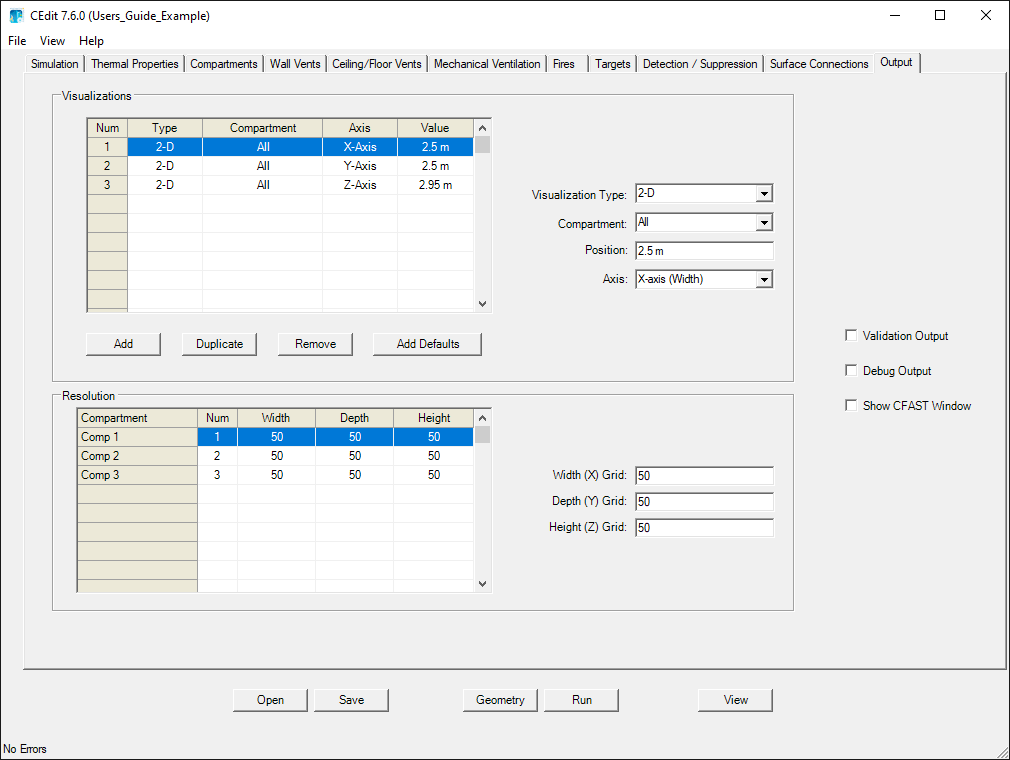
\includegraphics[width=6.5in]{FIGURES/Input_File/Visualizations_Tab}
\end{center}
\end{figure}

\section{Adding Visualizations}

\begin{description}
\item[Visualization Type] (default units: n/a, default value: 2-D): The type of visualization to be included. Choose from 2-D (a single plane slice of temperature at the position and axis specified), 3-D (a set of three animated slices whose position can be moved along its respective axis, or Isosurface (a fixed 3-D surface where the gas temperature is equal to the value specified. See the Smokeview documentation \cite{Smokeview_Users_Guide_6}for details on the use of Smokeview.

\item[Compartment] (default units: n/a, default value: All): Visualizations can be placed in a single compartment or at the same position and axis in all compartments.

\item[Position] (default units: m, default value: 0m): Position along the specified axes where the slice is placed measured from the compartment origin for the selected axis (0,0,0 is the bottom left corner of the compartment. See page \pageref{Compartment_Geometry}).

\item[Axis] (default units: n/s, default value: X-axis (Width)): Axis that the specified slice file is located.  The slice is place perpendicular to the selected axis (the Y-Z plane for the X-Axis; the X-Z plane for the Y-Axis, and the X-Y plane for the Z-Axis)

\item[Temperature] (default units \degc, default value: none): Specified gas temperature for the selected isosurface.
\end{description}

\graybox{
Use the Add Defaults button to add a default set of visualizations for the current simulation. A slice file entry is created at the center of each compartment in the x (width) and y (depth) directions along with one near the ceiling in the z direction. a 3-D slice file entry is created for each compartment as well.
}

\section{Visualization Resolution}

By default, slice files are generated with a grid of 50 data points in each direction for each compartment specified. If desired, the grid spacing can be adjusted up or down individually by compartment. Specifying a larger number of data points can \textit{dramatically} slow program execution since the gas temperature and velocity is evaluated at each grid location every time a Smokeview output is specified.  The default value should be appropriate for most simulations.

\begin{description}
\item[Width (X) Grid] (default units: n/a, default value: 50): slices included along the X axis for each compartment are uniformly divided into the specified number of data points.

\item[Width (Y) Grid] (default units: n/a, default value: 50): slices included along the Y axis for each compartment are uniformly divided into the specified number of data points.

\item[Width (Z) Grid] (default units: n/a, default value: 50): slices included along the Z axis for each compartment are divided into the specified number of data points.
\end{description}

Sample visualizations are included below.

\begin{figure}[h!]
\begin{center}
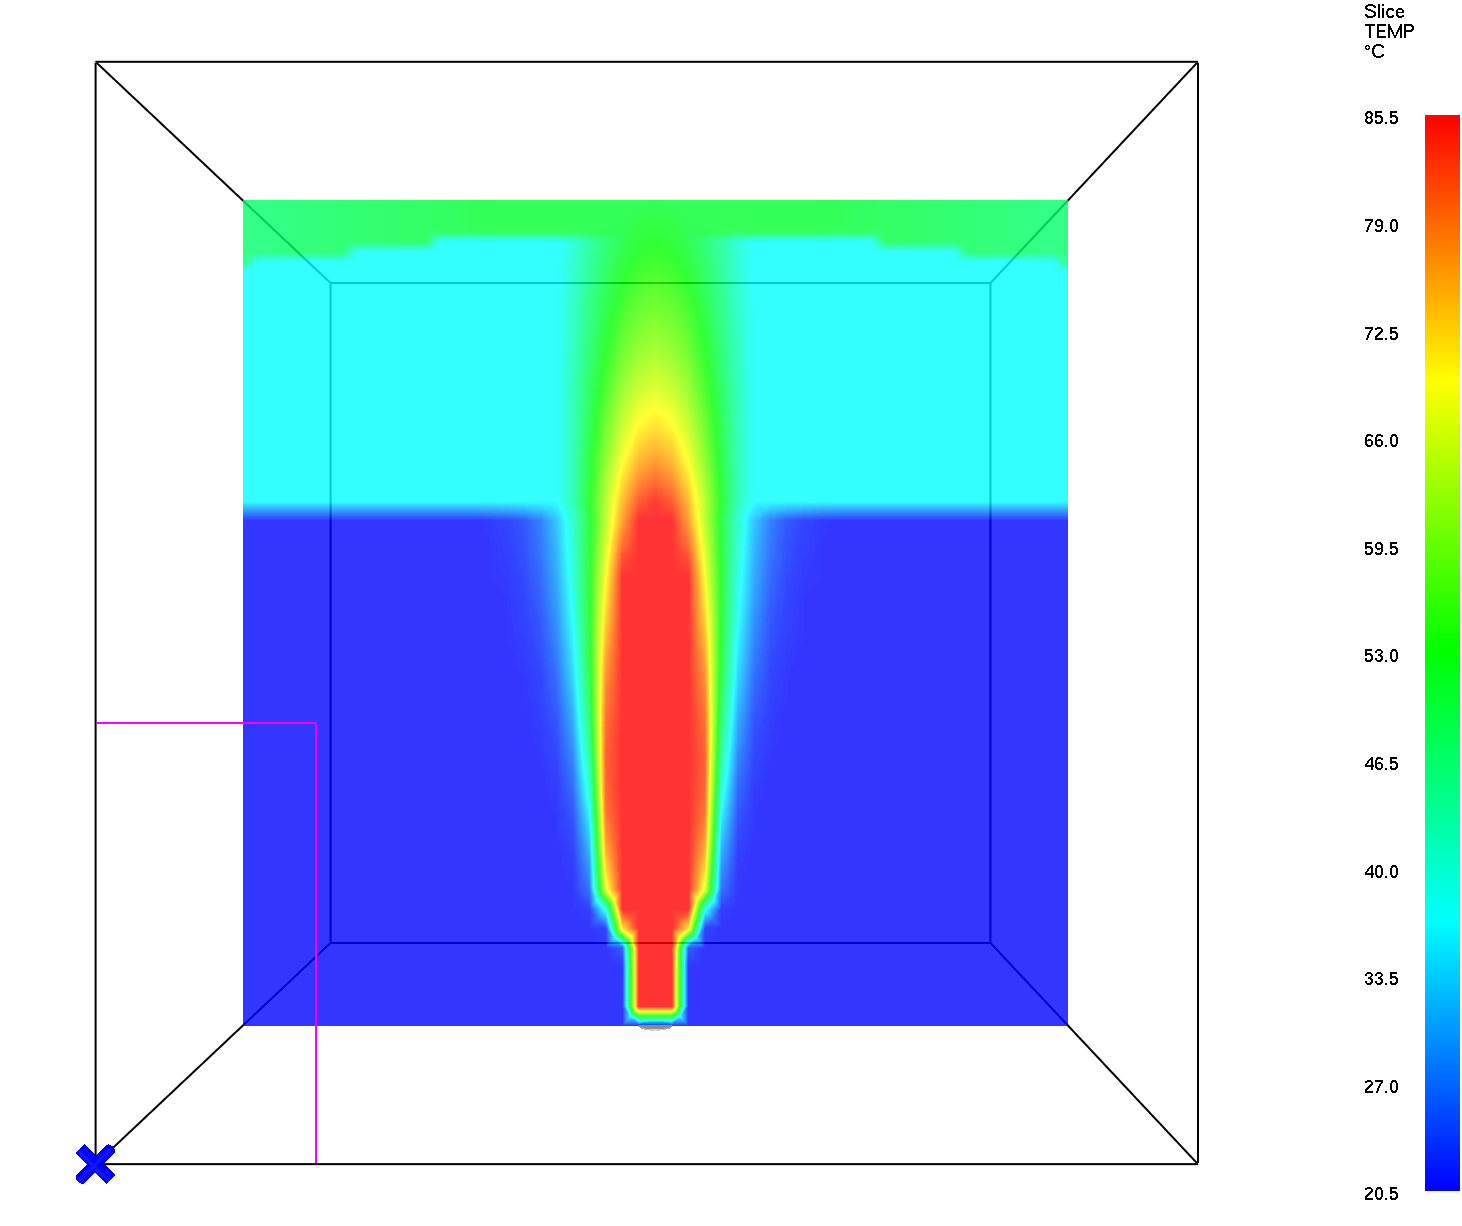
\includegraphics[width=6.5in]{FIGURES/Input_File/SMV_Temperature}
Smokeview Visualization of Gas Temperature with a Single Fire
\end{center}
\end{figure}

\begin{figure}[h!]
\begin{center}
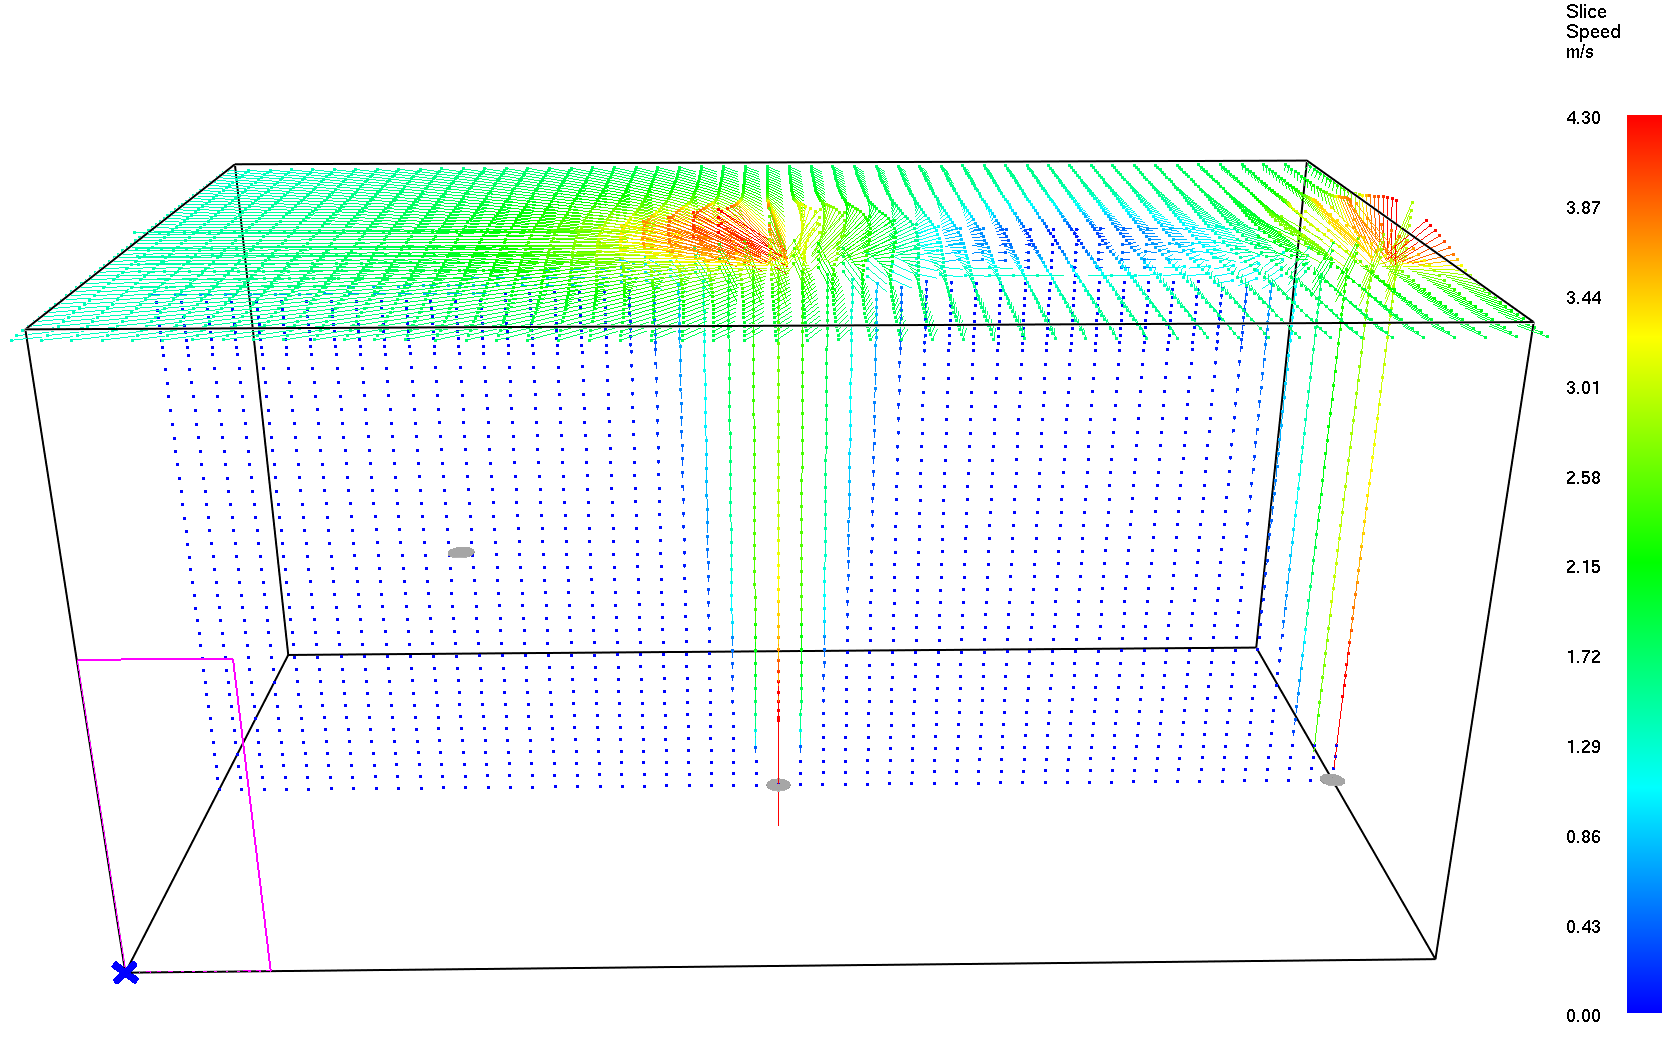
\includegraphics[width=6.5in]{FIGURES/Input_File/SMV_Velocity}
Smokeview Visualization of Gas Velocity with Two Fires
\end{center}
\end{figure}

\begin{figure}[h!]
\begin{center}
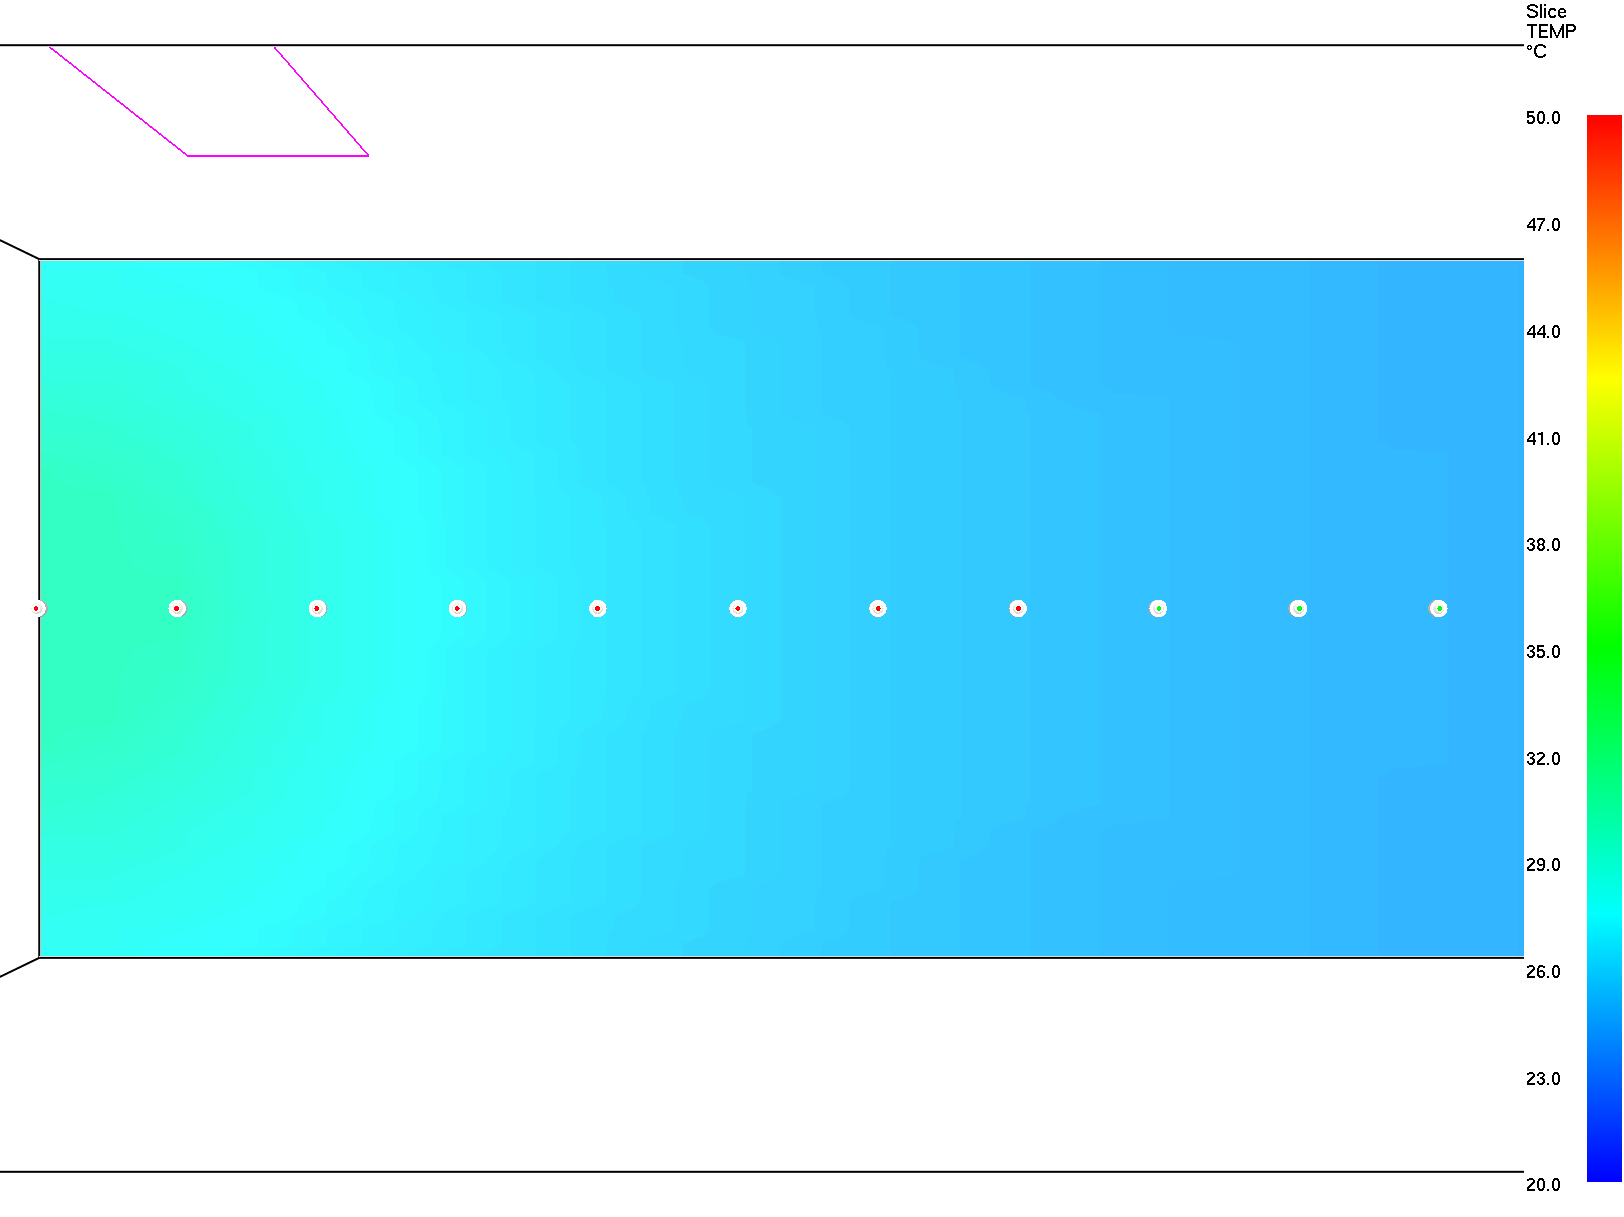
\includegraphics[width=6.5in]{FIGURES/Input_File/SMV_Detectors}
Smokeview Visualization of Detector Activation in a Corridor
\end{center}
\end{figure}


\chapter{Output from CFAST}
\label{Output_Chapter}

The output of CFAST includes the temperatures of the upper and lower gas layers within each compartment, the ceiling/wall/floor temperatures within each compartment, the visible smoke and gas species concentrations within each layer, target temperatures and sprinkler activation time.  The amount of information can be very large, especially for complex geometries and long simulations.

\section{Compact Output}

The default output to the console is called the compact form, and shows the basic information about a scenario, including layer temperatures and the size of fires. Default text output provides a simple overview for the user to make sure the case runs as expected.
\begin{lstlisting}[basicstyle=\scriptsize]
 Time =   1800.0 seconds.

 Compartment   Upper   Lower   Inter.  Pyrol     Fire      Pressure  Ambient
               Temp.   Temp.   Height  Rate      Size                Target
               (C)     (C)     (m)     (kg/s)    (W)       (Pa)      (W/m^2)
 -----------------------------------------------------------------------------
    1          113.4    33.3    1.4     1.393E-02 3.000E+05-0.790      523.
  Outside                                         0.00
\end{lstlisting}
The first column contains the compartment number.  On each row with its compartment number from left to right is the upper layer temperature, lower layer temperature, the height of the interface between the two layers, the total pyrolysis rate, and finally the total fire size.  The only value given for the outside is the total heat release rate of fires venting to the outside.

\section{Detailed Outputs}

The following sections describe each of the outputs from the model.  Each section refers to a specific part of the print out and appears in the order the output appears. A description of each option follows.

\subsection{Output for Initialization}

This option prints the initial conditions to the output before the actual run starts.  This merely mimics the inputs specified by the user in the input data file  The initial conditions brake down into seven sections.  Each is described below with the section name. The following explanation uses the output from the case STANDARD.IN. STANDARD.IN is included in the distribution. Please note, there are no mechanical ventilation, horizontal vents or detectors in this example, so the section discussing these phenomena are from additional data files.

\subsubsection{Overview}

The overview gives a general description of the case.  The output is fairly self explanatory. ``Doors, ...'' is the total number of horizontal natural flow vent connections in all compartments of the simulation.  ``Ceil. Vents, ...'' gives the total number of vertical natural flow vent connections in all compartments of the simulation.  The last header on the line ``MV Connections'' has the total number mechanical flow connections to all compartments in the simulation. Times in these outputs come from the TIMES input. All times are in s.
\begin{lstlisting}[basicstyle=\scriptsize]
 OVERVIEW


 Compartments    Doors, ...    Ceil. Vents, ...    MV Connects
    1               1             0                    0

 Simulation     Output         Smokeview      Spreadsheet
 Time           Interval       Interval       Interval
 (s)            (s)            (s)            (s)
   1800         120             10             30
\end{lstlisting}

\subsubsection{Ambient Conditions}

This section, like the overview section, needs little elaboration.  It gives the starting atmospheric conditions for the simulation both for outside and inside the structure. Data for these outputs come from the TAMB and EAMB inputs. Temperatures are in K, pressure in Pa, elevations in m, and wind speed in m/s. Wind Power is the dimensionless power law coefficient from the WIND input.
\begin{lstlisting}[basicstyle=\scriptsize]
 AMBIENT CONDITIONS

 Interior       Interior       Exterior       Exterior
 Temperature    Pressure       Temperature    Pressure
   (C)            (Pa)           (C)            (Pa)

     20.          101300.          20.          101300)
\end{lstlisting}

\subsubsection{Compartments}

The compartments section gives a summary of the geometry for the simulation.  A simple table summarizes the geometry with compartments running down the page in numerical order.  The various dimensions for each compartment are on the row with its compartment number.  Two columns need explanation.  The second to last column ``Ceiling Height'' gives the height of the ceiling relative to the station height in the Ambient Conditions section.  Similarly the ``Floor Height'' refers to the height of the floor above the station height.

\begin{lstlisting}[basicstyle=\scriptsize]
COMPARTMENTS

Compartment  Name                Width        Depth        Height       Ceiling      Floor
                                                                        Height       Height
                                 (m)          (m)          (m)          (m)          (m)
------------------------------------------------------------------------------------------------
    1        Compartment 1        9.10         5.00         4.60         4.60         0.00
\end{lstlisting}


\subsubsection{Horizontal Natural Ventilation}

This is the first table in the vent connections section.  Each row in the table characterizes one vent.  The first two columns contain the two compartments connected by the vent.  Each vent is ordered first by the lower number of the two compartments and then the numeric order of the second compartment.  The third column gives the vent number.  Column four is the width of the vent.  The next two columns report the sill and soffit height for the vent relative to the floor of the first compartment.  The seventh and eighth columns have a second listing of the sill and soffit height, this time relative to the station height.  Area of the vent is in the last column.

\begin{lstlisting}[basicstyle=\scriptsize]
VENT CONNECTIONS

Horizontal Natural Flow Connections (Doors, Windows, ...)

From           To             Vent       Width       Sill        Soffit      Abs.        Abs.
Compartment    Compartment    Number                 Height      Height      Sill        Soffit
                                         (m)         (m)         (m)         (m)         (m)
----------------------------------------------------------------------------------------------------
Compartment 1   Outside        1          1.00        0.00        2.40        0.00        2.40
\end{lstlisting}
From compartment, to compartment, vent number, width, sill height, and soffit height all come directly from the HVENT specifications in the input data file. Absolute sill height and absolute soffit height is the station elevation + compartment floor height + sill height. Absolute soffit height and absolute soffit height is the station elevation + compartment floor height + soffit height

\subsubsection{Vertical Natural Ventilation}

The first column is the upper compartment.  The upper compartment is the compartment where the vent opens into the floor.  The second column is the lower compartment where the vent is in the ceiling.  The third column describes the shape of the vent, which can be either round or square.  The fourth column gives the area of the vent.  The last two columns are the height of the vent, relative to the floor of the lower room and relative to the station height respectively.
\begin{lstlisting}[basicstyle=\scriptsize]
Vertical Natural Flow Connections (Ceiling, ...)

Top            Bottom         Shape     Area      Relative  Absolute
Compartment    Compartment                        Height    Height
                                        (m^2)     (m)       (m)
----------------------------------------------------------------------
 Outside           1          Round      1.00      4.60      4.60
\end{lstlisting}
Top compartment, bottom compartment, shape, and area come from the VVENT specifications in the input data file. Relative height is the height of the vent above the floor of the bottom compartment and absolute height is the height of the vent above the station elevation.

\subsubsection{Mechanical Flow Connections}

This section lists all connections to compartments and fans that connect between compartments. The first five columns in the fan table appear almost the same as the connections and ducts table.  The table lists, in order, the number of the system the fan is a part, the ``from'' node and its height, the ``to'' node and its height.  A fan actually draws air from the first or ``from'' node and pushes it to the second or ``to'' node.  In the second table, the headers give the direction of the flow of air.  The sixth column is the fan number as defined in CEdit.  The next two columns are the minimum and maximum pressures at which the fan curve is defined.  The rest of the row is made up of the two to five fan curve coefficients in the input file.

\begin{lstlisting}[basicstyle=\scriptsize]
FANS

System    From           From      To             To        Fan       Minimum   Maximum    Fan Curve
                         Elev.                    Elev.     Number
                         (m)                      (m)                 (Pa)      (Pa)
----------------------------------------------------------------------------------------------------
   1      Comp  1        1.00      Node  1        1.00                0.05
          Node  1        1.00      Node  2       10.00        1       200.00    300.00     3.80E-02
          Node  2       10.00      Outside       10.00                0.05
\end{lstlisting}

\subsubsection{Thermal Properties}

The thermal properties section brakes into two parts.  The first part is a table that lists the material for each surface of each compartment.  The compartments appear as rows down the page in numerical order.  From left to right next to the compartment number comes the material for the ceiling, wall and floor.  The second part lists the entries in the thermal data base.  The first line gives the database file used.  Next comes a listing of each material used. In addition to materials for compartment surfaces, any materials specified for targets are also listed.  For each listing of a material, the name is followed by the conductivity, specific heat, density, thickness and emissivity.

\begin{lstlisting}[basicstyle=\scriptsize]
 THERMAL PROPERTIES

 Compartment    Ceiling      Wall         Floor
 ----------------------------------------------------
 Compartment 1  GLASSFB3     CONCRETE     CONCRETE


 Thermal data base used: thermal

 Name    Conductivity Specific heat     Density     Thickness   Emissivity
 CONCRETE     1.75        1.000E+03    2.200E+03    0.150        0.940
 GLASSFB3    3.600E-02     795.         105.        1.300E-02    0.900
 METHANE     7.000E-02    1.090E+03     930.        1.270E-02    4.000E-02
 HARDWOOD    0.160        1.255E+03     720.        1.900E-02    0.900
 DEFAULT     0.120         900.         800.        1.200E-02    0.900
\end{lstlisting}
Material choices of the ceiling, walls, and floors come from the CEILI, WALLS, and FLOOR specifications in the input data file. Units for thermal properties are standard S.I. units.  For thermal conductivity, W/m K; for specific heat, J/kg K; for density, kg/m3; for thickness, m; emissivity is dimensionless.


\subsubsection{Targets}

The entry for targets shows the orientation of additional targets specified in the data file. Targets explicitly specified in the data file are listed first in the order they are included in the data file.  Each target is numbered based on the order of the target specifications in the input data file.  The compartment number, position of the target within the compartment, direction of the front face of the target object expressed as a normal unit vector to the surface, and object material. Additional targets, one for each compartment and one for each fire are automatically generated by the program and included in the list after the user-specified targets.

\begin{lstlisting}[basicstyle=\scriptsize]
TARGETS

Target Compartment    Position (x, y, z)         Direction (x, y, z)      Material
----------------------------------------------------------------------------------
    1    Compartmen   2.20     1.88     2.34     0.00     0.00     1.00   CONCRETE
    2    Compartmen   4.55     2.50     0.00     0.00     0.00     1.00   METHANE
    3    Compartmen   4.55     2.50     0.00     0.00     0.00     1.00   HARDWOOD
    4    Compartmen   4.55     2.50     0.00     0.00     0.00     1.00   CONCRETE
\end{lstlisting}
All of the inputs for targets come from the TARGE command in the input data file. Direction is specified as a unit vector as described in the section on target input. Units for position and direction are all in m.


\subsubsection{Fires}

The fire section lists all the information about the main fire and any object fires that might exist.  All the information for each fire is listed separately.  If there is a main fire, it comes first.  Each fire listing has the same form.  First is the name of the fire followed by a list of general information.  Listed left to right is the compartment the fire is in, the type of fire, the x, y, z position, the relative humidity, the lower oxygen limit, and finally the radiative fraction for the fire.

A table of time history curves for the fire follows.  The table contains all the time history curves for the fire.  Each row on the table is a specific time given in the left most column.  The rest of the columns give the values at that particular time.  The column headers indicate each input quantity and correspond to specific keywords in the fire definition.The headings include: Fmdot is pyrolysis rate; Hcomb is heat of combustion; Fqdot is heat release rate; Fheight is height of fire; Soot is fraction of the fuel mass converted to soot during combustion; CO is the fraction of the fuel mass converted to carbon monoxide during combustion, HCN is the fraction of the fuel mass converted to hydrogen cyanide during combustion, HCl is the fraction of the fuel mass converted to hydrogen chloride during combustion, CT is the concentration-time product, and TS is the fraction of fuel mass converted to trace species during combustion.

\begin{lstlisting}[basicstyle=\tiny]
FIRES

Name: bunsen   Referenced as object #  1

Compartment    Fire Type       Position (x,y,z)     Relative    Lower O2    Radiative
                                                    Humidity    Limit       Fraction
Compartment 1  Constrained     4.55   2.50   0.00   50.0        10.00        0.33


Chemical formula of the fuel
  Carbon    Hydrogen  Oxygen    Nitrogen  Chlorine
  1.000     4.000     0.000     0.000     0.000


  Time      Fmdot     Hcomb     Fqdot     Fheight   Soot      CO        HCN       HCl       CT        TS
  (s)       (kg/s)    (J/kg)    (W)       (m)       (kg/kg)   (kg/kg)   (kg/kg)   (kg/kg)   (kg/kg)   (kg/kg)
----------------------------------------------------------------------------------------------------------------
     0.      0.0      5.00E+07   0.0       0.0       0.0      1.05E-03   0.0       0.0       1.0       0.0
    60.     2.00E-03  5.00E+07  1.00E+05   0.0       0.0      1.05E-03   0.0       0.0       1.0       0.0
   120.     3.00E-03  5.00E+07  1.50E+05   0.0       0.0      1.05E-03   0.0       0.0       1.0       0.0
   180.     4.00E-03  5.00E+07  2.00E+05   0.0       0.0      1.05E-03   0.0       0.0       1.0       0.0
   240.     3.00E-03  5.00E+07  1.50E+05   0.0       0.0      1.05E-03   0.0       0.0       1.0       0.0
   300.     2.50E-03  5.00E+07  1.25E+05   0.0       0.0      1.05E-03   0.0       0.0       1.0       0.0
   360.     2.00E-03  5.00E+07  1.00E+05   0.0       0.0      1.05E-03   0.0       0.0       1.0       0.0
   420.     1.80E-03  5.00E+07  9.00E+04   0.0       0.0      1.05E-03   0.0       0.0       1.0       0.0
   480.     1.60E-03  5.00E+07  8.00E+04   0.0       0.0      1.05E-03   0.0       0.0       1.0       0.0
   540.     1.50E-03  5.00E+07  7.50E+04   0.0       0.0      1.05E-03   0.0       0.0       1.0       0.0
  1800.     1.50E-03  5.00E+07  7.50E+04   0.0       0.0      1.05E-03   0.0       0.0       1.0       0.0


Name: Wood_Wall   Referenced as object #  2

Compartment    Fire Type       Position (x,y,z)     Relative    Lower O2    Radiative
                                                    Humidity    Limit       Fraction
Compartment 1  Constrained     4.55   2.50   0.00   50.0        10.00        0.33


Chemical formula of the fuel
  Carbon    Hydrogen  Oxygen    Nitrogen  Chlorine
  6.000    10.000     5.000     0.000     0.000


  Time      Fmdot     Hcomb     Fqdot     Fheight   Soot      CO        HCN       HCl       CT        TS
  (s)       (kg/s)    (J/kg)    (W)       (m)       (kg/kg)   (kg/kg)   (kg/kg)   (kg/kg)   (kg/kg)   (kg/kg)
----------------------------------------------------------------------------------------------------------------
     0.      0.0      1.81E+07   0.0       0.0      2.00E-02  2.00E-02   0.0       0.0       1.0       0.0
  8000.     5.52E-02  1.81E+07  1.00E+06   3.0      2.00E-02  2.00E-02   0.0       0.0       1.0       0.0
\end{lstlisting}
All of the inputs for the main fire come from the fire specifications in the input data file. Data for the object fire comes from the object data file included with the CFAST software. Units for most values are included in the output.  Fire position is in m, relative humidity is in \%, lower oxygen limit is in volume percent, and pyrolysis temperature is in K.


\subsection{Output for Main Variables}

An expanded version of the compact default output called the normal print out can be obtained using the /f option.  When requested, the normal print out is the first information printed at each interval.  This information include the layer temperatures, interface height, volume of the upper layer, layer absorption coefficients, and compartment pressure (relative to ambient).

\begin{lstlisting}[basicstyle=\scriptsize]
 Time =   1800.0 seconds.

 Compartment   Upper     Lower     Inter.    Upper           Upper      Lower     Pressure
               Temp.     Temp.     Height    Vol.            Absorb     Absorb
                (C)      (C)       (m)       (m^3)           (m^-1)     (m^-1)      (Pa)
 ------------------------------------------------------------------------------------------
 Compartment 1  113.4    33.30     1.410     1.45E+02( 69%)  0.124      8.817E-02  -0.790
\end{lstlisting}
The second table of the normal print out has information about the fires.  In essence it is two tables joined.  The first part lists information by fire.  It starts with the main fire, if there is one, and then the object fires down the page.  The fires are listed in the second column followed by the plume flow rate, the pyrolysis rate and the fire size.  The next three columns are then skipped.  The next column with information is the amount of heat given off by each fire convectively, followed by the amount of heat given off radiantly.  The second part starts after all the fires have been individually listed.  It gives the totals for all fires in each compartment.  The first column has the compartment number.  The compartments start at one and are listed down the page in order.  The third to fifth columns are the same as the first part except the values are totals for the compartment and not just for one fire.  The sixth column has the total heat release rate that occurs in the upper layer.  The next column has the same total in the lower layer.  The eighth column has the total size of vent fires in the compartment.  Two columns of the table gives the convective and radiative parts of the fire heat release. The last two columns give the total mass pyrolyzed and the amount of trace species produced.

\begin{lstlisting}[basicstyle=\tiny]
 FIRES

 Compartment   Fire      Plume    Pyrol     Fire      Flame    Fire in  Fire in   Vent    Convec.   Radiat.   Pyrolysate  Trace
                         Flow     Rate      Size      Height   Upper    Lower     Fire
                         (kg/s)   (kg/s)    (W)       (m)      (W)      (W)       (W)       (W)       (W)       (kg)      (kg)
 -------------------------------------------------------------------------------------------------------------------------------
                burner   0.585    1.500E-03 7.500E+04 0.807                               5.025E+04 2.475E+04  3.13        0.00
              wood_wal   0.437    1.243E-02 2.250E+05 0.397                               1.507E+05 7.425E+04  11.2        0.00

 Compartment 1            1.02    1.393E-02 3.000E+05           0.00    3.000E+05  0.00
\end{lstlisting}
Flame height is calculated from the work of Heskestad~\cite{Heskestad:2002}. The average flame height is defined as the distance from the fuel source to the top of the visible flame where the intermittency is 0.5.  A flame intermittency of 0.5 means that the visible flame is above the mean 50~\% of the time and below the mean 50~\% of the time.


\subsection{Output for Wall Surfaces, Targets, and Detectors/Sprinklers}

The /f option provides two tables displaying information about wall surface or target temperatures and fluxes, and heat detectors or sprinklers. The left most column specifies the compartment number; followed by four columns providing the temperatures of the bounding surfaces of the compartment in contact with the ceiling, upper wall surface (in contact with the upper layer gases), lower wall surface (in contact with the lower layer gases), and floor, in that order. Next comes information about targets in the compartment, with each target listed on a separate line.  Information in the columns includes the surface temperature of the target, net heat flux to the target, and the percentage of that net flux that is due to radiation from the fire, radiation from compartment surfaces, radiation from the gas layers, and convection from the gas surrounding the target.  CFAST includes one target in the center of the floor for all compartments. Information on additional targets specified by the user in the input data file are also included, in the order specified in the input file.

\begin{lstlisting}[basicstyle=\tiny]
SURFACES AND TARGETS


Compartment  Ceiling Up wall Low wall Floor Target Gas   Surface Center Flux To Fire      Surface Gas
             Temp.   Temp.   Temp.    Temp.        Temp. Temp.   Temp.  Target  Rad.      Rad.    Rad.    Convect.
             (C)     (C)     (C)      (C)          (C)   (C)     (C)    (W/m^2) (W/m^2)   (W/m^2) (W/m^2) (W/m^2)
------------------------------------------------------------------------------------------------------------------
Compartment 1 23.0    22.5    21.6     22.6  Floor       22.6            17.8   2.817E-02  13.3    1.25    3.23
                                             1     23.7  21.7    20.9    23.2   0.00       12.0    1.54    9.67
                                             2     21.2  21.7    21.7    16.6   1.341E-04  12.0    1.46    3.23
                                             3     21.2  25.0    25.0    16.6   1.341E-04  12.0    1.46    3.23
\end{lstlisting}

\begin{lstlisting}[basicstyle=\scriptsize]
DETECTORS/ALARMS/SPRINKLERS

                             Sensor                           Smoke
Number  Compartment   Type   Temp (C)   Activated       Temp (C)   Vel (m/s)
----------------------------------------------------------------------------
 1        1           HEAT   2.627E+01  YES             2.518E+01  6.617E-01
\end{lstlisting}
In all cases, the flux to/from a target is net radiation or net convection. That is, it is the incoming minus the outgoing. So while a target or object is heating, the flux will be positive, and once it starts to cool, the flux will be negative. Values for radiation from fires (fire rad.), radiation from surfaces (surface rad.), radiation from the gas layers (gas rad.), and convection from surfaces (convect) are expressed as the net flux to target (flux to target). Positive values indicate heat gains by the target and negative values indicate heat losses.


\subsection{Output for Gas Species}

The /f option has two tables displaying information about the amounts of species in each layer. The species information follows the normal print out.  The first table gives species volume fractions for the upper layers of all the compartments and the second reports the same for the lower layers of all the compartments.  Again the compartments are listed down the page and the information across the page.  The species are each given in one of several different terms.  Below each header are the units for the given value.  Most of the headers are simply the chemical formula for the species being tracked.  However, several are not obvious.  ``TUHC'' is the total unburned hydrocarbons or the pyrolyzed fuel that hasn't burned yet.  ``OD'' is the obscuration density, which is a measure of the amount of smoke. ``TS'' is trace species.

\begin{lstlisting}[basicstyle=\scriptsize]
UPPER LAYER SPECIES

compartment   N2    O2     CO2       CO    HCN   HCL   TUHC H2O   OD        CT         TS
              (%)   (%)    (%)       (ppm) (ppm) (ppm) (%)  (%)   (1/m)     (g-min/m3) kg
----------------------------------------------------------------------------------------------
Compartment 1 79.2  20.5  9.055E-02  2.98  0.00  0.00  0.00 0.180 1.086E-02 51.8       0.00


LOWER LAYER SPECIES

compartment   N2    O2    CO2        CO     HCN   HCL   TUHC H2O   OD        CT         TS
              (%)   (%)   (%)        (ppm)  (ppm) (ppm) (%)  (%)   (1/m)     (g-min/m3) kg
----------------------------------------------------------------------------------------------
Compartment 1 79.3  20.7  6.412E-03  0.211  0.00  0.00  0.00 0.029 7.750E-04 4.00      0.00
\end{lstlisting}
The report by species for nitrogen, oxygen, hydrogen chloride and the total unburned hydrocarbons (fuel vapor in the layer) are percent by volume. Carbon dioxide, carbon monoxide and hydrogen cyanide are in parts per million, which is also a volume fraction.  Optical depth per meter is a measure of the visibility in the smoke. This is covered in detail in the comment on visibility in the section on fires and species specification. The concentration-time (CT) calculation is an integration of the species input for type CT (See section  for the input of CT) and is intended to represent a relative dose of toxic gas species . Trace species (TS) is the total kilograms of the trace species that is present in the compartment. It is an absolute measure and not percent or density.


\subsection{Output for Vent Flows}

Information about vent flow is obtained by using this option.  It includes a section detailing mass flow through horizontal, vertical, and mechanical vents. There are two forms for the vent flow. The first is flow through the vents as mass per second. The alternative, obtained used the / T option, gives the total mass which has flowed through the vent(s) and the relative mass of trace species divided by the total mass of trace species produced up this time.

The section for vent flow is titled ``FLOW THROUGH VENTS (kg/s).''  Because flow is always given in positive values, each vent is listed twice, once for flow going from compartment A to compartment B (labelled as ``Flow relative to `from''') and a second time for flow from B to A (labelled as ``Flow relative to `To'''.  As the example below shows, the first column lists the compartment.  The second column specifies the vent, including the type of vent (an ``H'' in this column stands for horizontal flow, such as through a doorway or window; a ``V'' here would mean vertical flow, such as through an opening in the ceiling, and an ``M'' stands for a mechanical ventilation connection) and the compartment from which the flow comes. Up to six additional columns detail the flow at this vent. Flow into and out of the compartment through the vent in the upper and lower layers are included, along with mixing between layers at the vent into the upper layer and into the lower layer.

\begin{lstlisting}[basicstyle=\tiny]
 FLOW THROUGH VENTS (kg/s)

                                        Flow relative to 'From'                Flow Relative to 'To'
                                        Upper Layer               Lower Layer  Upper Layer               Lower Layer
 Vent From/Bottom    To/Top     Inflow  Outflow      Inflow       Outflow      Inflow       Outflow      Inflow       Outflow
---------------------------------------------------------------------------------------------------------------------------------
 H  1 Compartment    Outside            1.000        0.974                     1.000                                  0.974
\end{lstlisting}
The mass balance is the sum of the flow in minus the flow out. (Note that this is an extended run to achieve results close to steady state.) For any compartment, this is just (Upper Layer Inflow + Lower Layer Inflow + Pyrol Rate) – (Upper Layer Outflow + Lower Layer Outflow) with the inflow and outflow summed for each vent. For the above example, the mass balance is:
$$(0.974 + 0.01393)~\hbox{kg/s} - (1.000)~\hbox{kg/s} = -0.012~\hbox{kg/s}$$
where the pyrolysis rate (from the ``normal'' output) is 0.01393 kg/s. The result is about the right magnitude (about 1 \% of the mass flow into or out of the vent) for net mass loss.  The mass loss should still be slightly negative since the compartment continues to heat.

An alternative printout is provided by use of the ``/t'' option. This shows total (mass) flow through vents. At present this is confined to mechanical ventilation. It applies only to vents which can be filtered, in this case mechanical ventilation. The last column is obtained by summing the outflow/inflow for each vent and then dividing that sum by the total trace species produced by all fires. For details on this value, see the section on output listing for fires.

\begin{lstlisting}[basicstyle=\tiny]
Total mass flow through vents (kg)

To             Through              Upper Layer               Lower Layer           Trace Species
Compartment    Vent             Inflow       Outflow      Inflow       Outflow      Relative to Total Release
-----------------------------------------------------------------------------------------------------
Compart        M Node  1                    63.9                      28.3          0.971

Compart        M Node  2                                 92.2                       0.971
\end{lstlisting}



\section{Spreadsheet Output}

CFAST can generate a number of output files in a plain text spreadsheet format.  These files capture a snap shot of the modeling data at an instant of time. This instance is determined by the fourth entry on the TIMES line of the data file. \emph{however}, there are events which can occur in between these reporting periods. Examples are the ignition of objects and the activation of detectors or sprinklers. These are \emph{not} reported in these output files.

\subsection{Primary Output Variables (project\_n.csv)}

There are two sets of information. The first is the compartment information such as layer temperature. This is output by compartment and there are eight entries for each compartment plus column that indicates the current simulation time:

\begin{description}
\item[Time] (s)
\item[Upper Layer Temperature] (\degc)
\item[Lower Layer Temperature] (\degc)
\item[Layer Height]  (m)
\item[ Upper Layer Volume] (m$^3$): total volume of the upper layer. This is just the floor area times the difference between the ceiling height and the layer height.
\item[ Pressure] (Pa): pressure at compartment floor relative to the outside at the absolute height of the floor.
\item[Ambient Temp Target Flux] (W/m$^2$): net heat flux to the center of the floor assuming the floor is at ambient temperature.  This is largely useful to estimate the tenability of the compartment.
\item[Floor Temp Target Flux] (W/m$^2$): net heat flux to the center of the floor.
\item[HRR Door Jet Fires] (W): total heat release rate of all doors jet fires \emph{adding} heat to this compartment.
\end{description}
The second section is for fires. There are seven entries per fire.  This information is displayed for each fire :
\begin{description}
\item[Plume Entrainment Rate] (kg/s): current mass entrained from the lower layer into the plume for this fire.
\item[Pyrolysis Rate] (kg/s): current rate of mass loss for this fire.
\item[HRR] (W): current total heat release rate for this fire. This is just the sum of the heat release rate for the lower layer and upper layer for this fire.
\item[HRR Lower] (W): current heat release rate for burning in the lower layer for this fire.
\item[HRR Upper] (W):  current heat release rate for burning in the upper layer for this fire.
\item[Flame Height] (m): current calculated flame height for this fire.
\item[Convective HRR] (W): current rate of heat release by convection for this fire.  The remainder is released by radiation to the surroundings.
\item[Total Pyrolysate Released] (kg): total mass released by the fire up to the current time.
\item[Total Trace Species Released] (kg): total mass of trace species released by the fire up to the current time.
\end{description}

\subsection{Species Output (project\_s.csv}

At present, the nine species, oxygen (O2), carbon dioxide (CO2), carbon monoxide (CO),  hydrogen cyanide (HCN), hydrogen chloride (HCL), water vapor (H2O), optical depth (OD), concentration-time dose (CT) and trace species (TS) are listed. This set of nine is enumerated for the upper and lower layer, and are done sequentially by compartment.
\begin{description}
\item[Time] (s)
\item[O2 Upper/Lower Layer] (mol \%): oxygen concentration in the upper (or lower) layer in the current compartment
\item[CO2 Upper/Lower Layer] (mol \%):  carbon dioxide concentration in the upper (or lower) layer in the current compartment
\item[CO Upper/Lowerr Layer] (ppm):  carbon monoxide concentration in the upper (or lower) layer in the current compartment
\item[HCN Upper/Lower Layer] (ppm):  HCN concentration in the upper (or lower) layer in the current compartment
\item[HCL Upper/Lower Layer] (ppm):  HCl concentration in the upper (or lower) layer in the current compartment
\item[H2O Upper/Lower Layer] (mol \%):  water vapor concentration in the upper (or lower) layer in the current compartment
\item[Optical Density Uppe/Lowerr Layer] (m$^{-1}$):  optical density in the upper (or lower) layer in the current compartment
\item[C-T Product Upper/Lower Layer] (g-min/m$^3$):  integrated concentration-time product in the upper (or lower) layer in the current compartment
\item[Trace Species Upper/Lower Layer] (kg):  total mass of trace species in the upper (or lower) layer in the current compartment
\end{description}

\subsection{Vent Flow (project\_f.csv)}

The first columns pertain to the horizontal flow through vertical vents such as windows and doors. There are two types of output, first to and from the outside, and second for interior compartments. The flow is broken down to flow in and out of the compartments. For flow to and from the outside (compartment N) there are two entries.
\begin{description}
\item[Time] (s)
\item[HVENT Inflow Vent \# 1 Outside-1] (kg/s): mass flow into the current compartment through the current horizontal flow (door/windows) vent connected to the current compartment
\item[HVENT Outflow Vent \# 1 Outside-1] (kg/s): mass flow out of the current compartment through the current horizontal flow (door/windows) vent connected to the current compartment
\end{description}
For interior compartments, there are additional entries for mixing entrainment into the upper and lower layers. Please see the technical reference guide for a detailed description of these flow fields.
\begin{description}
\item[HVENT Mixing to Upper Layer Vent \# 2 2-1] (kg/s): mass flow entrained from the lower to the upper layer by mixing at the current horizontal flow (door/windows) vent connected to the current compartment
\item[HVENT Mixing to Upper Layer Vent \# 2 2-1] (kg/s): mass flow entrained from the upper to the lower layer by mixing at the current horizontal flow (door/windows) vent connected to the current compartment
\end{description}
The second set of columns pertain to the vertical flow through horizontal vents. There are two entries for each vent in each compartment, showing the total flow into or out of each vent in each compartment.
\begin{description}
\item[VVENT Inflow Vent \# 1-Outside] (kg/s):  mass flow into the current compartment through the current vertical flow (ceiling/floor) vent connected to the current compartment
\item[VVENT Outflow Vent \# 1-Outside Vent Connection at Node 1-2] (kg/s):  mass flow out of the current  compartment through the current vertical flow (ceiling/floor) vent connected to the current compartment
\end{description}
The third set of columns pertain to the mechanical ventilation. Once again, there will be an entry for each node/compartment pair, showing the total flow into or out of the compartment through this node. In addition, the total amount of trace species through filters and captured on filters in mechanical ventilation connected to the compartment is included.
\begin{description}
\item[MVENT Inflow Vent Connection at Node 1-2] (kg/s): mass flow into the current compartment through the current mechanical flow (HVAC) vent connected to the current compartment
\item[MVENT Outflow] (kg/s): current mass flow out of the compartment through the current mechanical flow (HVAC) vent connected to the current compartment
\item[MVENT Trace Species Flow Fan at Node 2] (kg/s): current total mass of trace species flowing through the filter at the fan in the current mechanical vent connected to the current compartment
\item[MVENT Trace Species Filtered Fan at Node 2] (kg/s): total mass of trace species captured on the filter at the fan in the current mechanical vent connected to the current compartment
\end{description}

\subsection{Surface and Target Temperature and Heat Flux (project\_w.csv)}

This file provides information on surface and target temperatures and flux, and reports on the current state of detectors and sprinklers (as a sub-set of detectors). The output is in three sections, one for wall surface temperatures, one for target temperature and heat flux, and one for detector/sprinkler temperature and activation. The first set of columns pertain to the temperature of compartment surfaces.
\begin{description}
\item[Time] (s)
\item[Ceiling Temperature] (\degc): temperature of the ceiling surface in the current compartment
\item[Upper Wall Temperature] (\degc): temperature of the wall surface adjacent to the upper layer in the current compartment
\item[Lower Wall Temperature] (\degc): temperature of the  wall surface adjacent to the lower layer in the current compartment
\item[Floor Temperature] (\degc): temperature of the floor surface in the current compartment
\end{description}
The second set of columns pertain to the targets included in the simulation.  User-defined targets are list first followed by automatically-defined targets, one at the center of each compartment at floor level and one at the location of each fire in the simulation.
\begin{description}
\item[Target Surrounding Gas Temperature] (\degc): gas temperature nearby the current target
\item[Target Surface Temperature] (\degc): temperature of the surface of the current target
\item[Target Center Temperature] (\degc): interior temperature of the current target
\item[Target Total Flux] (kW/m$2$): total net heat flux to the front surface of the current target
\item[Target Convective Flux] (kW/m$2$): convective heat flux to the  front surface of the current target
\item[Target Radiative Flux] (kW/m$2$): radiative heat flux to the front surface of the current target
\item[Target Fire Radiative Flux] (kW/m$2$): radiative heat flux from fires to the front surface of the current target
\item[Target Surface Radiative Flux] (kW/m$2$): radiative heat flux from compartment surfaces to the front surface of the current target
\item[Target Gas Radiative Flux] (kW/m$2$):   radiative heat flux from the upper and lower gas layers to the front surface of the current target
\end{description}
The third set of columns pertain to the detector/sprinkler output.
\begin{description}
\item[Sensor Temperature] (\degc): temperature of the current detector / sprinkler
\item[Sensor Activation] (none): indicator of activation of the current detector / sprinkler; takes a value of zero if the sensor has not activated and one if it has
\item[Sensor Surrounding Gas Temperature] (\degc): gas temperature nearby the current detector / sprinkler. This is the ceiling jet temperature at the device location if the device is in the ceiling jet or the appropriate gas layer temperature if the device is lower in the compartment
\item[Sensor Surrounding Gas Velocity] (m/s): gas velocity nearby the current detector / sprinkler. The is the velocity of the ceiling jet at the device location if the device is in the ceiling jet or a default value of 0.1 m/s if the device is lower in the compartment
\end{description}

\newpage

\section{Error Messages}

In some (hopefully rare) cases, a simulation will fail to complete. In those cases, an error message provides guidance to the user on possible reasons for the failure. The message will contain an error number which provides a reference to additional information from the table below. Most often, these errors result from improper information in the input data files.
During initialization of the program for a simulation, CFAST may stop with an error message if the simulation cannot be initialized due to a missing or incorrect file specification. The error codes are as follows:
\begin{description}
\item[100] program called with no arguments (no input file)
\item[101] internal error in fire input; code for a free burning fire should not be reachable
\item[102] project file does not exist
\item[103] total file name length including path  is more than 256 characters
\item[104] one of the output files is not accessible (for example, if a CFAST case with this name is already running)
\item[105] error writing to an output file (openoutputfiles)
\item[106] a system fault has occurred. Applies to all open/close pairs once the model is running
\item[107] incompatible options
\item[108] not currently used
\item[109] cannot find/open a file
\item[110] error in handling the status input/output
\end{description}
Error codes from 1 to 99 are from the routine which parses the input and will be reported in the .log file.  The first set indicates a command with the wrong number of arguments. These errors indicate an error in a particular input command as follows:
\begin{description}
\item[1] TIMES command
\item[2] TAMB command
\item[3] EAMB command
\item[4] LIMO2 command
\item[5] THERMAL or FIRE commands
\item[7] MAINF command
\item[8] COMPA command
\item[10] HVENT command
\item[11] EVENT command
\item[12] MVENT command
\item[23] VVENT command
\item[24] WIND command
\item[25] INTER command
\item[26] MVOPN command
\item[28] MVDCT command
\item[29] MVFAN command
\item[32] OBJECT command
\item[34] CJET and DETEC command
\item[35] STPMAX command
\item[37] VHEAT command
\item[39] ONEZ command
\item[41] TARGE command
\item[46] HALL command
\item[47] ROOMA command
\item[51] ROOMH command
\item[55] DTCHE command
\item[56] SETP command
\item[58] HHEAT command
\item[65] HEATF command
\end{description}
The second set of errors related to parsing the input indicate specific errors with a command as follows:
\begin{description}
\item[9, compa] Compartment out of range
\item[26, inter] Not a defined compartment
\item[27, mvopn] Specified node number too large for this system
\item[30, mvfan] Fan curve has incorrect specification
\item[31, mvfan] Exceeded allowed number of fans
\item[33, object] Object must be assigned to an existing compartment
\item[35, detect] Invalid DETECTOR specification
\item[36, detect] A referenced compartment is not yet defined
\item[38, vheat] VHEAT has specified a non-existent compartment
\item[42, target] Too many targets are being defined
\item[43, target] The compartment specified by TARGET does not exist
\item[44, target] Invalid TARGET solution method specified
\item[45,  target] Invalid equation type specified in TARGET
\item[49, rooma] Compartment specified by ROOMA does not exist
\item[52, roomh] Compartment specified by ROOMH is not defined
\item[53, roomh] ROOMH error on data line
\item[54, roomh] Data on the ROOMA (or H) line must be positive
\item[57, setp] Trying to reset the SETP parameters
\item[61, hheat] HHEAT specification error in compartment pairs
\item[62, hheat] Error in fraction for HHEAT
\item[63, object] Fire type out of range
\item[64, object] The fire must be assigned to an existing compartment
\item[66, heatf] The heat source must be assigned to an existing compartment
\item[67, mvent] Compartment has not been defined
\item[68, mvent] Exceed one of the array bounds, ierror=68 (external), 69 (internal)  and 70 (fan)
\item[71, event] Undefined vent type
\item[72, inter] Specification for interface height is outside of allowable range
\item[73, inter] Compartments must be defined in pairs
\item[74, setp] The requested “SETP” command does not exists
\item[75, setp] Incorrect file reference
\item[76, setp] Cannot read the parameter file
\item[77, setp] Unsupported parameter
\end{description}
Errors 400 and above are failures while the model is running. 610 through 685 are failures in the numerical routines; these are rarely seen, but typically an internal error in the model.




%\backmatter


\bibliography{../Bibliography/CFAST_refs}

\appendix
\addcontentsline{toc}{chapter}{Appendices}

\chapter{Scenario and Software Limits}

CFAST is intended for use with a wide variety of fire scenarios.  A number of limits to the inputs in the software implementation of the model are noted below.


\begin{center}
\begin{tabular}{|p{15cm}|c|}
\hline
Maximum simulation time in seconds & 86400 \\ \hline
Maximum number of compartments & 100 \\ \hline
Maximum number of horizontal flow (door/window) vent connections that can be included in a single test case & 2500 \\ \hline
Maximum number of vertical flow (ceiling/floor) vent connections which can be included in a single test case & 2500 \\ \hline
Maximum total number of connections between compartments and mechanical ventilation systems which can be included in a single test case & 2500 \\ \hline
Maximum number of fans that can be included in a single test cases  & 1250 \\ \hline

Maximum number of fires which can be included in a single test case & 2500 \\ \hline
Maximum number of data points for a single  fire definition & 199 \\ \hline
Maximum number of data points in a variable cross-sectional area definition for a single compartment & 199 \\ \hline
Maximum number of material thermal property definitions which can be included in a single thermal database file & 2500 \\ \hline

Maximum number of targets which can be included in a single test case. In addition, the CFAST model includes a target on the floor of each compartment in the simulation and one for each object fire in simulation. & 2500 \\ \hline
Maximum number of detectors/sprinklers which can be included in a single test case. & 2500 \\ \hline

\hline
\end{tabular}
\end{center} 

\clearpage
\chapter{CFAST Text-based Input File}

The operation of CFAST is based on a single ASCII\footnote{ASCII -- American Standard Code for Information Interchange. There are 256 characters that make up the standard ASCII text.} text file containing parameters organized into {\em namelist}\footnote{A {\em namelist} is a Fortran input record.} groups.
The input file provides CFAST  with all of the necessary information to describe the scenario. The graphical user interface, CEdit, writes this file. This appendix details all the parameters, which are organized into groups that roughly coincide with the tabs in the graphical user interface.

\section{Naming the Input File}

The input file is saved with a name such as {\ct job\_name.in}, where {\ct job\_name} is any character string that helps to identify the simulation. All of the output files associated with the calculation will then have this common prefix name.

There should be no blank spaces in the job name. Instead use the underscore character to represent a space.

Be aware that CFAST will simply over-write the output files of a given case if its assigned name is the same. This is convenient when developing an input file because you save on disk space. Just be careful not to overwrite a calculation that you want to keep.

\section{Namelist Formatting}

Parameters are specified within the input file by using {\em namelist} formatted records. Each namelist record begins with the ampersand character, {\ct \&}, followed immediately by the name of the namelist group, then a comma-delimited list of the input parameters, and finally a forward slash, {\ct /}. For example, the line
\begin{lstlisting}
&TIME  SIMULATION = 3600., PRINT = 50., SMOKEVIEW = 50., SPREADSHEET = 50. /
\end{lstlisting}
sets various values of parameters contained in the {\ct TIME} namelist group. The meanings of these various parameters is explained in this guide. The namelist records can span multiple lines in the input file, but just be sure to end the record with a slash or else the data will not be understood. Do not add anything to a namelist line other than the parameters and values appropriate for that group. Otherwise, CFAST will stop immediately upon execution.

Parameters within a namelist record can be separated by either commas, spaces, or line breaks. It is recommended that you use commas or line breaks, and never use tab stops because they are not explicitly defined in the namelist data structure. CFAST and CEdit expect the first character of the file to be an ampersand, {\ct \&}, and by convention the first namelist is the {\ct HEAD} namelist but any namelist can be the first. Comments and notes can be written into the file between namelists so long as nothing comes before the ampersand except a space and nothing comes between the ampersand and the slash except appropriate parameters corresponding to that particular namelist group. However, it is important to note that any comments in an  input file that is opened by CEdit and saved will be lost.

The parameters in the input file can be integers, reals, character strings, or logical parameters. A logical parameter is either {\ct .TRUE.} or {\ct .FALSE.} -- the periods are a Fortran convention. Character strings that are listed in this User's Guide must be copied exactly as written -- the code is case sensitive and underscores {\em do} matter. The maximum length of most character input parameters is 60.

Most of the input parameters are simply real or integer scalars, like {\ct PRINT = 50.}, but sometimes the inputs can be arrays.

Note that character strings can be enclosed either by single or double quotation marks, however CEdit only recognizes the single quotation mark. Be careful not to create the input file by pasting text from something other than a simple text editor, in which case the punctuation marks may not transfer properly into the text file. Some text file encodings may not work on all systems. If file reading errors occur and no typographical errors can be found in the input file, try saving the input file using a different encoding. For example, the text file editor Notepad works fine on a Windows PC, but a file edited in Notepad may not work on Linux or Mac OS~X because of the difference in line endings between Windows and Unix/Linux operating systems. The editor Wordpad typically works better, but try a simple case first.


\section{Input File Structure}

In general, the namelist records can be entered in any order in the input file, but it is a good idea to organize them in some systematic way. Typically, general information is listed near the top of the input file, and detailed information, like obstructions, devices, and so on, are listed below. CFAST scans the entire input file each time it processes a particular namelist group. With some text editors, it has been noticed that the last line of the file is often not read by CFAST because of the presence of an ``end of file'' character. To ensure that CFAST reads the entire input file, add
\begin{lstlisting}
&TAIL /
\end{lstlisting}
as the last line at the end of the input file. This completes the file from {\ct \&HEAD} to {\ct \&TAIL}. CFAST does not even look for this last line. It just forces the ``end of file'' character past relevant input.

The general structure of an input file is shown below, with many lines of the original input file\footnote{The actual input file, Users\_Guide\_Example.in, is part of the CFAST software distribution} removed for clarity.

%\clearpage
\begin{lstlisting}[basicstyle=\tiny]
&HEAD VERSION = 7300, TITLE = 'Users Guide Example Case' /
!! Scenario Configuration
&TIME SIMULATION = 3600 PRINT = 50 SMOKEVIEW = 50 SPREADSHEET = 50 /
&INIT PRESSURE = 101325 RELATIVE_HUMIDITY = 50 INTERIOR_TEMPERATURE = 20 EXTERIOR_TEMPERATURE = 20 /
&MISC  LOWER_OXYGEN_LIMIT = 0.1 /
!! Material Properties
&MATL ID = 'CONCRETE' MATERIAL = 'Concrete, Normal Weight (6 in)',
      CONDUCTIVITY = 1.75 DENSITY = 2200 SPECIFIC_HEAT = 1, THICKNESS = 0.15 EMISSIVITY = 0.94 /
!! Comparments
&COMP ID = 'Comp 1'
      DEPTH = 5 HEIGHT = 3 WIDTH = 5 CEILING_MATL_ID = 'CONCRETE' WALL_MATL_ID = 'CONCRETE' FLOOR_MATL_ID = 'CONCRETE'
      ORIGIN = 0, 0, 0 GRID = 50, 50, 50 /
!! Devices
&DEVC ID = 'HeatDetector_3' COMP_ID = 'Comp 1' LOCATION = 2, 2, 2.97 TYPE = 'HEAT_DETECTOR' SETPOINT = 30, RTI = 5 /
!! Wall Vents
&VENT TYPE = 'WALL' ID = 'WallVent_1' COMP_IDS = 'Comp 1' 'OUTSIDE'  TOP = 2, BOTTOM = 0, WIDTH = 1
      FACE = 'FRONT' OFFSET = 2 /
!! Fires
&FIRE ID = 'Wood_Wall' COMP_ID = 'Comp 2', FIRE_ID = 'Wood_Wall_Fire'  LOCATION = 2.5, 5 /
&CHEM ID = 'Wood_Wall_Fire' CARBON = 6 CHLORINE = 0 HYDROGEN = 10 NITROGEN = 0 OXYGEN = 5 HEAT_OF_COMBUSTION = 18100 RADIATIVE_FRACTION = 0.33 /
&TABL ID = 'Wood_Wall_Fire' LABELS = 'TIME', 'HRR' , 'HEIGHT' , 'AREA' , 'CO_YIELD' , 'SOOT_YIELD' , 'HCN_YIELD' , 'HCL_YIELD' , 'TRACE_YIELD' /
&TABL ID = 'Wood_Wall_Fire', DATA = 0, 0, 0, 0.05, 0.006171682, 0.015, 0, 0, 0 /
&TABL ID = 'Wood_Wall_Fire', DATA = 8000, 1000, 3, 9, 0.006171682, 0.015, 0, 0, 0 /
!! Surface Connections
&CONN TYPE = 'FLOOR' COMP_ID = 'Comp 3' COMP_IDS = 'Comp 2' /
!! Visualizations
&SLCF DOMAIN = '2-D'  POSITION = 2.5, PLANE = 'X' /
&TAIL /

\end{lstlisting}
It is recommended that when looking at a new scenario, first select a pre-written input file that resembles the case, make the necessary changes, then run the case to determine if the geometry is set up correctly. It is best to start off with a relatively simple file that captures the main features of the problem without getting tied down with too much detail that might mask a fundamental flaw in the calculation. As you learn how to write input files, you will continually run and re-run your case as you add in complexity.

Table~\ref{tbl:namelistgroups} provides a quick reference to all the namelist parameters and where you can find the reference to where it is introduced in the document and the table containing all of the keywords for each group.


\begin{table}[ht]
\begin{center}
\caption{CFAST Input File Keywords}
\label{tbl:namelistgroups}
\begin{tabular}{|c|l|c|c|}
\hline
Group Name   & Namelist Group Description     & Reference Section & Parameter Table  \\ \hline
{\ct COMP}   & Compartments                   & \ref{info:COMP}   & \ref{tbl:COMP}   \\ \hline
{\ct CHEM}   & Fire Chemistry                 & \ref{info:FIRE}   & \ref{tbl:FIRE}   \\ \hline
{\ct CONN}   & Surface Connections            & \ref{info:CONN}   & \ref{tbl:CONN}   \\ \hline
{\ct DEVC}   & Devices                        & \ref{info:DEVC}   & \ref{tbl:DEVC}   \\ \hline
{\ct DIAG}   & Diagnostics                    &                   & \ref{tbl:DIAG}   \\ \hline
{\ct FIRE}   & Fires Placement                & \ref{info:FIRE2}  & \ref{tbl:FIRE2}  \\ \hline
{\ct HEAD}   & Input File Header              & \ref{info:HEAD}   & \ref{tbl:HEAD}   \\ \hline
{\ct INIT}   & Initial Conditions             & \ref{info:INIT}   & \ref{tbl:INIT}   \\ \hline
{\ct ISOF}   & Isosurface File Outputs        & \ref{info:ISOF}   & \ref{tbl:ISOF}   \\ \hline
{\ct MATL}   & Material Properties            & \ref{info:MATL}   & \ref{tbl:MATL}   \\ \hline
{\ct MISC}   & Miscellaneous                  & \ref{info:MISC}   & \ref{tbl:MISC}   \\ \hline
{\ct SLCF}   & Slice File Outputs             & \ref{info:SLCF}   & \ref{tbl:SLCF}   \\ \hline
{\ct TAIL}   & End of Input File Indicator    &                   &                  \\ \hline
{\ct TABL}   & Table of Time-Based Inputs     & \ref{info:FIRE3}  & \ref{tbl:FIRE3}  \\ \hline
{\ct TIME}   & Simulation Time                & \ref{info:TIME}   & \ref{tbl:TIME}   \\ \hline
{\ct VENT}   & Vents                          & \ref{info:VENT}   & \ref{tbl:WVENT}  \\ \hline
\end{tabular}
\end{center}
\end{table}

Examples of each of the inputs are included in the sections that follow.  All examples are taken from the sample input file {\ct Users\_Guide\_Example.in} included with the CFAST distribution. Following are some general rules about the CFAST input file:

\begin{itemize}
\item The {\ct HEAD} input identifies the version of CFAST for which the input file was created and is typically the first line in the input file. Use {\ct \&TAIL} as the last line at the end of the input file. This completes the file from {\ct \&HEAD} to {\ct \&TAIL}. CFAST does not even look for this last line. It just forces the “end of file” character past relevant input.
\item Many of the listed keywords are mutually exclusive. Repeated entry of some keywords can cause the program to either fail or run in an unpredictable manner.
\item Use of some keywords triggers the code to operate in a certain mode/condition. For example, specifying {\ct ADIABATIC} to be {\ct .TRUE.} triggers the code to treat all compartment surfaces to be perfectly insulated.
\item Multiple inputs are required whenever the keyword is in plural form --- keywords ending with an \textbf{s}. For example, the keyword parameter, {\ct TEMPERATURES}, within the namelist group, {\ct INIT}, requires two temperature values (in this case, one for exterior ambient temperature and one for interior ambient temperature). In the case of missing inputs, an error message will be generated to assist users in troubleshooting any errors.
\item Default values to inputs are assigned to some of the keywords to facilitate the set up of an input file. For instance, Table \ref{tbl:MISC} shows that the {\ct LOWER\_OXYGEN\_LIMIT} has a default value of {\ct 0.15}. This value is taken from the SFPE handbook \cite{SFPE:2003} and implies that the burning rate will be reduced when the oxygen level is below 15~\%. Users should review the applicability of any default values for their simulation.
\end{itemize}


\clearpage

\section{Simulation Environment, Namelist Groups \texorpdfstring{{\tt HEAD}}{HEAD}, \texorpdfstring{{\tt TIME}}{TIME}, \texorpdfstring{{\tt INIT}}{INIT}, and  \texorpdfstring{{\tt MISC}}{MISC}}

\noindent
\renewcommand{\tabcolsep}{.1in}
\begin{longtable}{|l|l|l|l|l|}
\caption[Header Parameters ({\ct HEAD} namelist group)]{For more information see Section~\ref{info:HEAD}.}
\label{tbl:HEAD} \\
\hline
\multicolumn{5}{|c|}{{\ct HEAD} (Header Parameters)} \\
\hline \hline
\endfirsthead
\caption[]{Continued} \\
\hline
\multicolumn{5}{|c|}{{\ct HEAD} (Header Parameters)} \\
\hline \hline
\endhead
\parbox{1.5in}{\bf Parameter}    & \parbox{1in}{\bf Type}  & \parbox{1in}{\bf Reference}  & \parbox{1in}{\bf Units}  & \parbox{1in}{\bf Default Value} \\ \hline
{\ct VERSION}         & Integer                 & Section \ref{info:HEAD}      &         	     &                   \\ \hline
{\ct TITLE}           & Character               & Section \ref{info:HEAD}      &       		     &                 	 \\ \hline
\end{longtable}



\noindent
\begin{longtable}{@{\extracolsep{\fill}}|l|l|l|l|l|}
\caption[Time Parameters ({\ct TIME} namelist group)]{For more information see Section~\ref{info:TIME}.}
\label{tbl:TIME} \\
\hline
\multicolumn{5}{|c|}{{\ct TIME} (Time Parameters)} \\
\hline \hline
\endfirsthead
\caption[]{Continued} \\
\hline
\multicolumn{5}{|c|}{{\ct TIME} (Time Parameters)} \\
\hline \hline
\endhead
\parbox{1.5in}{\bf Parameter}    & \parbox{1in}{\bf Type}  & \parbox{1in}{\bf Reference}  & \parbox{1in}{\bf Units}  & \parbox{1in}{\bf Default Value} \\ \hline
{\ct PRINT}             & Integer   & Section \ref{info:TIME}                 & s         & 60              \\ \hline
{\ct SIMULATION}        & Integer   & Section \ref{info:TIME}                 & s         & 3600            \\ \hline
{\ct SMOKEVIEW}         & Integer   & Section \ref{info:TIME}                 & s         & 15              \\ \hline
{\ct SPREADSHEET}       & Integer   & Section \ref{info:TIME}                 & s         & 15              \\ \hline
\end{longtable}



\noindent
\begin{longtable}{@{\extracolsep{\fill}}|l|l|l|l|l|}
\caption[Initial Conditions ({\ct INIT} namelist group)]{For more information see Section~\ref{info:INIT}.}
\label{tbl:INIT} \\
\hline
\multicolumn{5}{|c|}{{\ct INIT} (Initial Conditions)} \\
\hline \hline
\endfirsthead
\caption[]{Continued} \\
\hline
\multicolumn{5}{|c|}{{\ct INIT} (Initial Conditions)} \\
\hline \hline
\endhead
\parbox{1.5in}{\bf Parameter}    & \parbox{1in}{\bf Type}  & \parbox{1in}{\bf Reference}  & \parbox{1in}{\bf Units}  & \parbox{1in}{\bf Default Value} \\ \hline
{\ct PRESSURE}                   & Real   		   & Section \ref{info:INIT}      & Pa       		     & 101325     		       \\ \hline
{\ct RELATIVE\_HUMIDITY}         & Real   		   & Section \ref{info:INIT}      & \%      		     & 50       		       \\ \hline
{\ct INTERIOR\_TEMPERATURE}       & Real  	       & Section \ref{info:INIT}      & $^\circ$C		     & 20      	   \\ \hline
{\ct EXTERIOR\_TEMPERATURE}       & Real            & Section \ref{info:INIT}      & $^\circ$C		     & 20      	   \\ \hline
\end{longtable}



\noindent
\begin{longtable}{@{\extracolsep{\fill}}|l|l|l|l|l|}
\caption[Miscellaneous Parameters ({\ct MISC} namelist group)]{For more information see Section~\ref{info:MISC}.}
\label{tbl:MISC} \\
\hline
\multicolumn{5}{|c|}{{\ct MISC} (Miscellaneous Parameters)} \\
\hline \hline
\endfirsthead
\caption[]{Continued} \\
\hline
\multicolumn{5}{|c|}{{\ct MISC} (Miscellaneous Parameters)} \\
\hline \hline
\endhead
\parbox{1.5in}{\bf Parameter}    & \parbox{1in}{\bf Type}  & \parbox{1in}{\bf Reference}  & \parbox{1in}{\bf Units}  & \parbox{1in}{\bf Default Value} \\ \hline
{\ct ADIABATIC}            & Logical     & Section \ref{info:MISC}                 &           & {\ct .FALSE.}   \\ \hline
{\ct LOWER\_OXYGEN\_LIMIT} & Real        & Section \ref{info:MISC}                 &           &   0.15          \\ \hline
{\ct MAX\_TIME\_STEP}      & Real        & Section \ref{info:MISC}                 & s         &   1             \\ \hline
{\ct MAX\_ITERATION}      & Real         & Section \ref{info:MISC}                 &           &   Unlimited     \\ \hline
{\ct OVERWRITE}            & Logical     & Section \ref{info:MISC}                 &           & {\ct .TRUE.}    \\ \hline
{\ct SPECIFIC\_EXTINCTION} & Real Doublet        & Section \ref{info:MISC}         &           &   8700,4400     \\ \hline
\end{longtable}

\noindent Examples:
\begin{lstlisting}
&HEAD  VERSION = 7300, TITLE = 'Users Guide Example Case' /
&TIME  SIMULATION = 3600., PRINT = 50., SMOKEVIEW = 50., SPREADSHEET = 50. /
&INIT  INTERIOR_TEMPERATURE = 20., EXTERIOR_TEMPERATURE = 20. /
&MISC  LOWER_OXYGEN_LIMIT = 0.10 /
\end{lstlisting}


\clearpage

\section{Thermal Properties, Namelist Group \texorpdfstring{{\tt MATL}}{MATL}}

\noindent
\begin{minipage}{6.5in}
\renewcommand\footnoterule{}
\begin{longtable}{@{\extracolsep{\fill}}|l|l|l|l|l|}
\caption[Thermal Properties ({\ct MATL} namelist group)]{For more information see Section~\ref{info:MATL}.}
\label{tbl:MATL} \\
\hline
\multicolumn{5}{|c|}{{\ct MATL} (Material Properties)} \\
\hline \hline
\endfirsthead
\caption[]{Continued} \\
\hline
\multicolumn{5}{|c|}{{\ct MATL} (Material Properties)} \\
\hline \hline
\endhead
\parbox{1.5in}{\bf Parameter}    & \parbox{1in}{\bf Type}  & \parbox{1in}{\bf Reference}  & \parbox{1in}{\bf Units}  & \parbox{1in}{\bf Default Value} \\ \hline
{\ct CONDUCTIVITY}*\footnote{ * indicates a required input for each {\ct MATL} input included in the input file.}       & Real 	 & Section \ref{info:MATL}                 & kW/(m$\cdot$K)  	&                 \\ \hline
{\ct DENSITY}*            & Real 	 & Section \ref{info:MATL}                 & kg/m$^3$ 		&                 \\ \hline
{\ct EMISSIVITY}          & Real	 & Section \ref{info:MATL}                 &         		&   0.9           \\ \hline
{\ct ID}*                 & Character    & Section \ref{info:MATL}                 &                    &                 \\ \hline
{\ct MATERIAL}*           & Character    & Section \ref{info:MATL}                 &                    &                 \\ \hline
{\ct SPECIFIC\_HEAT}*     & Real	 & Section \ref{info:MATL}                 & kJ/(kg$\cdot$K)    &                 \\ \hline
{\ct THICKNESS}*\footnote{ THICKNESS provides a default value for the material. It can be overridden for a specific compartment surface. For targets, the default value is used.}          & Real  	 & Section \ref{info:MATL}                 & m     	        &                 \\ \hline
\end{longtable}
\end{minipage}

\vspace{\baselineskip}
\noindent Example:
\begin{lstlisting}
&MATL ID = 'CONCRETE', MATERIAL = 'Light weight concrete',
      CONDUCTIVITY = 1.75, SPECIFIC_HEAT = 1.,
      DENSITY = 2200., EMISSIVITY = 0.94, THICKNESS = 0.15 /
\end{lstlisting}


\clearpage
\section{Compartments, Namelist Group \texorpdfstring{{\tt COMP}}{COMP}}

\noindent
\begin{minipage}{6.5in}
\renewcommand\footnoterule{}
%\begin{longtable}{@{\extracolsep{\fill}}|l|l|l|l|l|}
\begin{longtable}{|l|l|l|l|l@{\extracolsep{\fill}}|}
\caption[Compartment parameters ({\ct COMP} namelist group)]{For more information see Section~\ref{info:COMP}.}
\label{tbl:COMP} \\
\hline
\multicolumn{5}{|c|}{{\ct COMP} (Compartment Parameters)} \\
\hline \hline
\endfirsthead
\caption[]{Continued} \\
\hline
\multicolumn{5}{|c|}{{\ct COMP} (Compartment Parameters)} \\
\hline \hline
\endhead
\parbox{1.5in}{\bf Parameter}    & \parbox{1in}{\bf Type}  & \parbox{1in}{\bf Reference}  & \parbox{1in}{\bf Units}  & \parbox{1in}{\bf Default Value} \\ \hline
{\ct CEILING\_MATL\_ID}\footnote{ If included, from 1 to 3 material ids can each be input for the ceiling, floor, and walls.}     & Character Triplet		 & Section \ref{info:COMP2}               &           &                 \\ \hline
{\ct CEILING\_THICKNESS}\footnote{ If included, from 1 to 3 material thicknesses can each be input for the ceiling, floor, and walls. If a zero value is input, the default thickness for the material is used.}        & Real Triplet		 & Section \ref{info:COMP2}                 &           &                 \\ \hline
{\ct CROSS\_SECT\_AREAS}
\footnote{For compartments where the cross-sectional area varies with height, the inputs, {\ct CROSS\_SECT\_AREAS} and {\ct CROSS\_SECT\_HEIGHTS} can be used.}
                            & Real Array          & Section \ref{info:COMP4}                 &           &                 \\ \hline
{\ct CROSS\_SECT\_HEIGHTS}  & Real Array          & Section \ref{info:COMP4}                 &           &                 \\ \hline
{\ct DEPTH}*\footnote{ * indicates a required input for each {\ct COMP} input included in the input file. At least one {\ct COMP} input must be included in an input file.}                 & Real     		 & Section \ref{info:COMP}                & m         &  		\\ \hline
{\ct FLOOR\_MATL\_ID}       & Character Triplet		 & Section \ref{info:COMP2}               &           &                 \\ \hline
{\ct FLOOR\_THICKNESS}        & Real Triplet		 & Section \ref{info:COMP2}                 &           &                 \\ \hline
{\ct GRID}             & Integer Triplet& Section \ref{info:SLCF2}               &           & 50,50,50                \\ \hline
{\ct HALL}                  & Logical  		 & Section \ref{info:COMP3}               &           & {\ct .FALSE.}   \\ \hline
{\ct HEIGHT}*                & Real     		 & Section \ref{info:COMP}   	          & m         &                 \\ \hline
{\ct ID}*                    & Character		 & Section \ref{info:COMP}                &           &          \\ \hline
{\ct LEAK\_AREA}               & Real Doublet      & Section \ref{info:COMP}                & m$^2$/m$^2$          &          \\ \hline
{\ct ORIGIN}           & Real Triplet   & Section \ref{info:COMP}                & m         & 0,0,0                \\ \hline
{\ct SHAFT}                 & Logical  		 & Section \ref{info:COMP3}                 &           & {\ct .FALSE.}   \\ \hline
{\ct TYPE}                  & Character      & Section \ref{info:COMP}                &           &          \\ \hline
{\ct WALL\_MATL\_ID}        & Character Triplet		 & Section \ref{info:COMP2}                 &           &                 \\ \hline
{\ct WALL\_THICKNESS}        & Real Triplet		 & Section \ref{info:COMP2}                 &           &                 \\ \hline
{\ct WIDTH}*                 & Real               & Section \ref{info:COMP}                  & m         &                 \\ \hline
\end{longtable}
\end{minipage}

\vspace{\baselineskip}
\noindent Example:
\begin{lstlisting}
&COMP ID = 'Comp 1'
      DEPTH = 6.1 HEIGHT = 2.4 WIDTH = 3.7
      CEILING_MATL_ID = 'FiberCem' CEILING_THICKNESS = 0.025
      WALL_MATL_ID = 'FiberCem', 'Gypsum', 'Concrete'
      WALL_THICKNESS = 0.013, 0.03, 0.61
      FLOOR_MATL_ID = 'FiberCem', 'Gypsum', 'Concrete'
      FLOOR_THICKNESS = 0.013, 0.03, 0.61
      ORIGIN = 0, 0, 0 GRID = 50, 50, 50 LEAK_AREA_RATIO = 0, 0.0005 /
\end{lstlisting}




\clearpage
\section{Vents, Namelist Group \texorpdfstring{{\tt VENT}}{VENT}}
\label{info:VENT6}

\subsection{Wall Vents\texorpdfstring{{\tt ,TYPE='WALL'}}{, TYPE='WALL'}}

\noindent
\begin{minipage}{6.5in}
\renewcommand\footnoterule{}
\begin{longtable}{@{\extracolsep{\fill}}|l|l|l|l|l|}
\caption[Wall Vent Parameters ({\ct VENT} namelist group)]{For more information see Section~\ref{info:VENT}.}
\label{tbl:WVENT} \\
\hline
\multicolumn{5}{|c|}{{\ct VENT, TYPE='WALL'} (Wall Vent Parameters)} \\
\hline \hline
\endfirsthead
\caption[]{Continued} \\
\hline
\multicolumn{5}{|c|}{{\ct VENT, TYPE='WALL'} (Wall Vent Parameters)} \\
\hline \hline
\endhead
\parbox{1.5in}{\bf Parameter}    & \parbox{1in}{\bf Type}  & \parbox{1in}{\bf Reference}  & \parbox{1in}{\bf Units}  & \parbox{1in}{\bf Default Value} \\ \hline
{\ct BOTTOM}\footnote{ * indicates a required input for each wall {\ct VENT} input included in the input file.} *               & Real                   & Section \ref{info:VENT}      & m                        &                 \\ \hline
{\ct COMP\_IDS}*     	   			         & Character Doublet        & Section \ref{info:VENT}      &                             &                 \\ \hline
{\ct CRITERION}\footnote{Input for {\ct CRITERION} must be {\ct FLUX}, {\ct TEMPERATURE}, or {\ct TIME}. An associated {\ct SETPOINT} is required. For {\ct FLUX} or {\ct TEMPERATURE}, an associated ignition target must be specified by {\ct DEVC\_ID}.}
                            				         & Selection List              & Section \ref{info:VENT}      &                             &                 \\ \hline
{\ct DEVC\_ID}           					 & Character  		  & Section \ref{info:VENT}      &                             &                 \\ \hline
{\ct F}\footnote{Specifies the fraction of vent width for wall vents as a function of time and is only applicable when {\ct CRITERION} is set to {\ct TIME}. Must also include {\ct T}.}  					 & Real Array  		  & Section \ref{info:VENT}      &                             &                 \\ \hline
{\ct FACE}\footnote{Input for {\ct FACE} must be {\ct RIGHT}, {\ct FRONT}, {\ct LEFT}, or {\ct REAR}. Both {\ct FACE} and {\ct OFFSET} positioning refer to the first compartment specified ({\ct COMP\_IDS(1)}).}      	  & Selection List   & Section \ref{info:VENT}              &                             &                 \\ \hline
{\ct HEIGHT}*                 & Real                   & Section \ref{info:VENT}      & m                        &                 \\ \hline
{\ct ID}*                                                         & Character  	          & Section \ref{info:VENT}      &                             &                 \\ \hline
{\ct OFFSET}       					 & Real 		  & Section \ref{info:VENT}      & m                           &      0        \\ \hline
{\ct PRE\_FRACTION}\footnote{{\ct PRE\_FRACTION} and {\ct POST\_FRACTION} specify the vent fraction before and after the {\ct SETPOINT} is reached when {\ct CRITERION} is either {\ct TEMPERATURE} or {\ct FLUX}. They cannot be used with {\ct F} and {\ct T}.}       					 & Real 		  & Section \ref{info:VENT}      & m                           &      1        \\ \hline
{\ct POST\_FRACTION}       					 & Real 		  & Section \ref{info:VENT}      & m                           &      1        \\ \hline
{\ct SETPOINT}           					 & Real  	          & Section \ref{info:VENT}      & s $\mid$ $^\circ$C $\mid$ kW/m$^2$ &                 \\ \hline
{\ct T}  					 & Real Array  		  & Section \ref{info:VENT}      &                             &                 \\ \hline
{\ct TOP}*                 & Real                   & Section \ref{info:VENT}      & m                        &                 \\ \hline               &                             &                 \\ \hline
{\ct TYPE}\footnote{Input for {\ct TYPE} must be {\ct WALL} to specify a wall vent. } *
                                                                 & Selection List         & Section \ref{info:VENT6}     &                             &                 \\ \hline
{\ct WIDTH}*                                                      & Real                   & Section \ref{info:VENT}      & m                           &                 \\ \hline
\end{longtable}
\end{minipage}

\graybox{Wall vents ({\ct TYPE='WALL'}) are defined by {\ct BOTTOM}, {\ct TOP}, and {\ct WIDTH}. Location of the vent for visualization is defined by {\ct FACE}, and {\ct OFFSET}. \\
}

\noindent Example:
\begin{lstlisting}
&VENT TYPE = 'WALL', ID = 'HVENT 1', COMP_IDS = 'Comp 1', 'OUTSIDE',
      WIDTH = 1., TOP = 2., BOTTOM = 0.,
      OFFSET = 2., FACE = 'FRONT' /

\end{lstlisting}

\subsection{Ceiling / Floor Vents\texorpdfstring{{\tt ,TYPE='CEILING'} or {\tt TYPE='FLOOR'}}{{, TYPE='CEILING'} or {\tt TYPE='FLOOR'}}}

\noindent
\begin{minipage}{6.5in}
\renewcommand\footnoterule{}
\begin{longtable}{@{\extracolsep{\fill}}|l|l|l|l|l|}
\caption[Ceiling/Floor Vent Parameters ({\ct VENT} namelist group)]{For more information see Section~\ref{info:VENT}.}
\label{tbl:CFVENT} \\
\hline
\multicolumn{5}{|c|}{{\ct VENT, TYPE='CEILING'} or {\ct TYPE='FLOOR'} (Ceiling/Floor Vent Parameters)} \\
\hline \hline
\endfirsthead
\caption[]{Continued} \\
\hline
\multicolumn{5}{|c|}{{\ct VENT, TYPE='CEILING'} or {\ct TYPE='FLOOR'} (Ceiling/Floor Vent Parameters)} \\
\hline \hline
\endhead
\parbox{1.5in}{\bf Parameter}    & \parbox{1in}{\bf Type}  & \parbox{1in}{\bf Reference}  & \parbox{1in}{\bf Units}  & \parbox{1in}{\bf Default Value} \\ \hline
{\ct AREA}\footnote{ * indicates a required input for each ceiling/floor {\ct VENT} input included in the input file.} *      	 & Real  	          & Section \ref{info:VENT2}     & m$^2$                    &                                 \\ \hline
{\ct COMP\_IDS}*     	   			         & Character Doublet        & Section \ref{info:VENT}      &                             &                 \\ \hline
{\ct CRITERION}\footnote{Input for {\ct CRITERION} must be {\ct FLUX}, {\ct TEMPERATURE}, or {\ct TIME}. An associated {\ct SETPOINT} is required. For {\ct FLUX} or {\ct TEMPERATURE}, an associated ignition target must be specified by {\ct DEVC\_ID}.}
                            				         & Selection List              & Section \ref{info:VENT}      &                             &                 \\ \hline
{\ct DEVC\_ID}           					 & Character  		  & Section \ref{info:VENT}      &                             &                 \\ \hline
{\ct F}\footnote{Specifies the fraction of vent width for wall vents as a function of time and is only applicable when {\ct CRITERION} is set to {\ct TIME}. Must also include T.}  					 & Real Array  		  & Section \ref{info:VENT}      &                             &                 \\ \hline
{\ct ID}*                                                         & Character  	          & Section \ref{info:VENT}      &                             &                 \\ \hline
{\ct OFFSETS}       					 & Real Doublet 		  & Section \ref{info:VENT}      & m                           &      0,0        \\ \hline
{\ct PRE\_FRACTION}\footnote{{\ct PRE\_FRACTION} and {\ct POST\_FRACTION} specify the vent fraction before and after the {\ct SETPOINT} is reached when {\ct CRITERION} is either {\ct TEMPERATURE} or {\ct FLUX}. They cannot be used with {\ct F} and {\ct T}.}       					 & Real 		  & Section \ref{info:VENT}      & m                           &      1        \\ \hline
{\ct POST\_FRACTION}       					 & Real 		  & Section \ref{info:VENT}      & m                           &      1        \\ \hline
{\ct SHAPE}*\footnote{Input for {\ct SHAPE} must be {\ct ROUND} or {\ct SQUARE}.}
                                                                 & Selection List         & Section \ref{info:VENT2}     &                             &                 \\ \hline
{\ct T}  					 & Real Array  		  & Section \ref{info:VENT}      &                             &                 \\ \hline
{\ct TYPE}\footnote{Input for {\ct TYPE} must be {\ct CEILING} or {\ct FLOOR} for ceiling and floor vents. These may be used interchangeably. The order of {\ct COMP\_IDS} specifies the location of the vent with {\ct COMP\_IDS(1)} specifying the top compartment and {\ct COMP\_IDS(2)} specifying the bottom compartment.} *
                                                                 & Selection List         & Section \ref{info:VENT6}     &                             &                 \\ \hline
\end{longtable}
\end{minipage}

\graybox {Ceiling and floor vents ({\ct TYPE='CEILING'} or {\ct TYPE='FLOOR'}) are defined by {\ct AREA} and {\ct SHAPE}. Location of the vent for visualization is defined by {\ct OFFSETS} as the distance from the compartment origin in the X (width) and Y (depth) direction. It is visualized on the floor of {\ct COMP\_IDS(1)}. \\
}

\noindent Example:
\begin{lstlisting}
&VENT TYPE = 'CEILING', ID = 'VVENT 1', COMP_IDS = 'Comp 3', 'Comp 2',
      AREA = 1., SHAPE = 'ROUND', CRITERION= 'TIME',
      T = 0., 100., 500.,
      F = 0., 0.5, 1. /

\end{lstlisting}

\subsection{Mechanical Vents\texorpdfstring{{\tt ,TYPE='MECHANICAL'}}{, TYPE='MECHANICAL'}}

\noindent
\begin{minipage}{6.5in}
\renewcommand\footnoterule{}
\begin{longtable}{@{\extracolsep{\fill}}|l|l|l|l|l|}
\caption[Mechanical Vent Parameters ({\ct VENT} namelist group)]{For more information see Section~\ref{info:VENT}.}
\label{tbl:MVENT} \\
\hline
\multicolumn{5}{|c|}{{\ct VENT, TYPE='MECHANICAL'} (Mechanical Vent Parameters)} \\
\hline \hline
\endfirsthead
\caption[]{Continued} \\
\hline
\multicolumn{5}{|c|}{{\ct VENT, TYPE='MECHANICAL'} (Mechanical Vent Parameters)} \\
\hline \hline
\endhead
\parbox{1.5in}{\bf Parameter}    & \parbox{1in}{\bf Type}  & \parbox{1in}{\bf Reference}  & \parbox{1in}{\bf Units}  & \parbox{1in}{\bf Default Value} \\ \hline
{\ct AREAS}\footnote{ * indicates a required input for each mechanical {\ct VENT} input included in the input file.} *       & Real Doublet 	          & Section \ref{info:VENT3}     & m$^2$                    &                 \\ \hline
{\ct COMP\_IDS}*    	   			         & Character Doublet        & Section \ref{info:VENT}      &                             &                 \\ \hline
{\ct CRITERION}\footnote{Input for {\ct CRITERION} must be {\ct FLUX}, {\ct TEMPERATURE}, or {\ct TIME}. An associated {\ct SETPOINT} is required. For {\ct FLUX} or {\ct TEMPERATURE}, an associated ignition target must be specified by {\ct DEVC\_ID}.}
                            				         & Selection List              & Section \ref{info:VENT}      &                             &                 \\ \hline
{\ct CUTOFFS}       					 & Real Doublet 	  	  & Section \ref{info:VENT4}     & Pa                          &     200.,300.     \\ \hline
{\ct DEVC\_ID}           					 & Character  		  & Section \ref{info:VENT}      &                             &                 \\ \hline
{\ct F}\footnote{Specifies the fraction of vent width for wall vents as a function of time and is only applicable when {\ct CRITERION} is set to {\ct TIME}. Must also include {\ct T}.}  					 & Real Array  		  & Section \ref{info:VENT}      &                             &                 \\ \hline
{\ct FILTER\_TIME}    					 & Real  		  & Section \ref{info:VENT}      & s                            &  0               \\ \hline
{\ct FILTER\_EFFICIENCY}    					 & Real  		  & Section \ref{info:VENT}      & \% removed                            &  0.0               \\ \hline
{\ct FLOW}*      	 					 & Real  		  & Section \ref{info:VENT4}     & m$^3$/s                     &                 \\ \hline
{\ct HEIGHTS}*      					 & Real Doublet  	  & Section \ref{info:VENT3}     & m                           &                 \\ \hline
{\ct ID}*                                                         & Character  	          & Section \ref{info:VENT}      &                             &                 \\ \hline
{\ct OFFSETS}       					 & Real Doublet 		  & Section \ref{info:VENT}      & m                           &      0.,0.        \\ \hline
{\ct ORIENTATIONS}\footnote{Input for {\ct ORIENTATION} must be {\ct HORIZONTAL} or {\ct VERTICAL}}  					 & Selection List Doublet 		  & Section \ref{info:VENT}      &                             & {\tiny VERTICAL,VERTICAL}                \\ \hline
{\ct PRE\_FRACTION}\footnote{{\ct PRE\_FRACTION} and {\ct POST\_FRACTION} specify the vent fraction before and after the {\ct SETPOINT} is reached when {\ct CRITERION} is either {\ct TEMPERATURE} or {\ct FLUX}. They cannot be used with {\ct F} and {\ct T}.}       					 & Real 		  & Section \ref{info:VENT}      & m                           &      1        \\ \hline
{\ct POST\_FRACTION}       					 & Real 		  & Section \ref{info:VENT}      & m                           &      1        \\ \hline
{\ct SETPOINT}           					 & Real  	          & Section \ref{info:VENT}      & s $\mid$ $^\circ$C $\mid$ kW/m$^2$ &                 \\ \hline
{\ct T}  					 & Real Array  		  & Section \ref{info:VENT}      &                             &                 \\ \hline
{\ct TYPE}\footnote{Input for {\ct TYPE} must be {\ct MECHANICAL} for mechanical vents.} *
                                                                 & Selection List         & Section \ref{info:VENT6}     &                             &                 \\ \hline
\end{longtable}
\end{minipage}

\graybox{Mechanical vents {\ct TYPE='MECHANICAL'} are defined by {\ct AREAS}, {\ct CUTOFFS}, {\ct FLOW}, and {\ct HEIGHTS}. Location of the vent for visualization is defined by {\ct ORIENTATION} and {\ct OFFSETS} as the distance from the compartment origin in the X (width) and Y (depth) direction and by {\ct HEIGHTS(1)} in the z direction. \\
}

\noindent Example:
\begin{lstlisting}
&VENT TYPE = 'MECHANICAL', ID = 'MVENT_1',
      COMP_IDS = 'OUTSIDE', 'Comp 1', AREAS = 0.25, 0.25,
      HEIGHTS = 2.75, 2.75, FLOW = 0.02,
      CUTOFFS = 200., 300., ORIENTATION='VERTICAL', OFFSETS = 0., 4. /

\end{lstlisting}




\clearpage
\section{Fires, Namelist Groups \texorpdfstring{{\tt FIRE}}{FIRE}, \texorpdfstring{{\tt CHEM}}{CHEM},  and  \texorpdfstring{{\tt TABL}}{TABL}}
\label{info:FIRE3}

\noindent
\begin{minipage}{6.5in}
\renewcommand\footnoterule{}
\begin{longtable}{@{\extracolsep{\fill}}|l|l|l|l|l|}
\caption[Fire Parameters ({\ct FIRE} namelist group)]{For more information see Section~\ref{info:FIRE}.}
\label{tbl:FIRE2} \\
\hline
\multicolumn{5}{|c|}{{\ct FIRE} (Individual Instance of a Fire Object)} \\
\hline \hline
\endfirsthead
\caption[]{Continued} \\
\hline
\multicolumn{5}{|c|}{{\ct FIRE} (Individual Instance of a Fire Object)} \\
\hline \hline
\endhead
\parbox{1.5in}{\bf Parameter}    & \parbox{1in}{\bf Type}  & \parbox{1in}{\bf Reference}  & \parbox{1in}{\bf Units}  & \parbox{1in}{\bf Default Value} \\ \hline
{\ct COMP\_ID}\footnote{ * indicates a required input for each {\ct FIRE} input included in the input file.} *             & Character   & Section \ref{info:FIRE}                 &                             &                 \\ \hline
{\ct DEVC\_ID}             & Character   & Section \ref{info:FIRE}                 &                             &                 \\ \hline
{\ct FIRE\_ID}* & Character        & Section \ref{info:FIRE}                 &                        &            \\ \hline
{\ct ID}*                   & Character   & Section \ref{info:FIRE}                 &                             &                 \\ \hline
{\ct IGNITION\_CRITERION}\footnote{for {\ct IGNITION\_CRITERION} inputs must be{\ct TIME},{\ct TEMPERTURE}, or {\ct FLUX}}   & Selection List   & Section \ref{info:FIRE}                 &                             & {\ct TIME}                \\ \hline
{\ct LOCATION}*             & Real Pair        & Section \ref{info:FIRE}                 & m                           &                 \\ \hline
{\ct SETPOINT}             & Real        & Section \ref{info:FIRE}                 & s $\mid$ $^\circ$C $\mid$ kW/m$^2$  & 0 s        \\ \hline
\end{longtable}
\end{minipage}

\noindent
\begin{minipage}{6.5in}
\renewcommand\footnoterule{}
\begin{longtable}{@{\extracolsep{\fill}}|l|l|l|l|l|}
\caption[Fire Parameters ({\ct CHEM} namelist group)]{For more information see Section~\ref{info:FIRE}.}
\label{tbl:FIRE} \\
\hline
\multicolumn{5}{|c|}{{\ct CHEM} (Fire Chemistry Parameters)} \\
\hline \hline
\endfirsthead
\caption[]{Continued} \\
\hline
\multicolumn{5}{|c|}{{\ct CHEM} (Fire Chemistry Parameters)} \\
\hline \hline
\endhead
\parbox{1.5in}{\bf Parameter}    & \parbox{1in}{\bf Type}  & \parbox{1in}{\bf Reference}  & \parbox{1in}{\bf Units}  & \parbox{1in}{\bf Default Value} \\ \hline
{\ct CARBON}               & Real     & Section \ref{info:FIRE}                 &                             &  1               \\ \hline
{\ct CHLORINE}             & Real     & Section \ref{info:FIRE}                 &                             &  0               \\ \hline
{\ct FLAMING\_TRANSITION\_TIME} & Real     & Section \ref{info:FIRE}                 &                             &  0               \\ \hline
{\ct HEAT\_OF\_COMBUSTION} & Real        & Section \ref{info:FIRE}                 & kJ/kg                       &     50000       \\ \hline
{\ct HYDROGEN}             & Real     & Section \ref{info:FIRE}                 &                             &  4               \\ \hline
{\ct ID}\footnote{ * indicates a required input for each {\ct CHEM} input included in the input file.} *                  & Character   & Section \ref{info:FIRE}                 &                             &                 \\ \hline
{\ct NITROGEN}             & Real     & Section \ref{info:FIRE}                 &                             & 0                \\ \hline
{\ct OXYGEN}               & Real     & Section \ref{info:FIRE}                 &                             & 0                \\ \hline
{\ct RADIATIVE\_FRACTION}  & Real        & Section \ref{info:FIRE}                 &                             &     0.35        \\ \hline
\end{longtable}
\end{minipage}

\noindent
\begin{minipage}{6.5in}
\renewcommand\footnoterule{}
\begin{longtable}{@{\extracolsep{\fill}}|l|l|l|l|l|}
\caption[Fire Parameters ({\ct TABL} namelist group)]{For more information see Section~\ref{info:FIRE}.}
\label{tbl:FIRE3} \\
\hline
\multicolumn{5}{|c|}{{\ct TABL} (Time-Based Fire Chemistry Parameters)} \\
\hline \hline
\endfirsthead
\caption[]{Continued} \\
\hline
\multicolumn{5}{|c|}{{\ct FIRE} (Time-Based Fire Chemistry Parameters)} \\
\hline \hline
\endhead
\parbox{1.5in}{\bf Parameter}    & \parbox{1in}{\bf Type}  & \parbox{1in}{\bf Reference}  & \parbox{1in}{\bf Units}  & \parbox{1in}{\bf Default Value} \\ \hline
{\ct LABELS}               & Character Array        & Section \ref{info:FIRE}                 &                        &              \\ \hline
{\ct ID}\footnote{ * indicates a required input for each {\ct TABL} input included in the input file.} *                    & Character   & Section \ref{info:FIRE}                 &                             &                 \\ \hline
{\ct DATA}             & Real Array       & Section \ref{info:FIRE}                 &   &        \\ \hline
\end{longtable}
\end{minipage}

\clearpage
\noindent Example:
\begin{lstlisting}
&FIRE ID = 'Wood_Wall'
 COMP_ID = 'Comp 2', FIRE_ID = 'Wood_Wall_Fire'
 LOCATION = 2.5, 5 /
&CHEM ID = 'Wood_Wall_Fire'
 CARBON = 6, CHLORINE = 0, HYDROGEN = 10, NITROGEN = 0, OXYGEN = 5
 HEAT_OF_COMBUSTION = 18100,  RADIATIVE_FRACTION = 0.33 /
&TABL ID = 'Wood_Wall_Fire', LABELS = 'TIME', 'HRR', 'HEIGHT', 'AREA', 'CO_YIELD', 'SOOT_YIELD' /
&TABL ID = 'Wood_Wall_Fire', DATA =    0,      0,     0,        0.05,   0.00617,    0.015 /
&TABL ID = 'Wood_Wall_Fire', DATA =    8000,   1000,  3,        9,      0.00617,    0.015 /
\end{lstlisting}




\clearpage
\section{Devices, Namelist Group \texorpdfstring{{\tt DEVC}}{DEVC}}

\label{info:DEVC3}

\noindent
\begin{minipage}{6.5in}
\renewcommand\footnoterule{}
\begin{longtable}{@{\extracolsep{\fill}}|l|l|l|l|l|}
\caption[Device Parameters ({\ct DEVC} namelist group)]{For more information see Section~\ref{info:DEVC}.}
\label{tbl:DEVC} \\
\hline
\multicolumn{5}{|c|}{{\ct DEVC} (Device Parameters)} \\
\hline \hline
\endfirsthead
\caption[]{Continued} \\
\hline
\multicolumn{5}{|c|}{{\ct DEVC} (Device Parameters)} \\
\hline \hline
\endhead
\parbox{1.5in}{\bf Parameter}    & \parbox{1in}{\bf Type}  & \parbox{1in}{\bf Reference}  & \parbox{1in}{\bf Units}  & \parbox{1in}{\bf Default Value} \\ \hline
{\ct ADIABATIC\_TARGET}\footnote{If included, inputs for {\ct CONVECTION\_COEFFICENTS} are required.}           					 & Logical  		  & Section \ref{info:DEVC}      &                             &  {\ct .FALSE.}     \\ \hline
{\ct CONVECTION\_COEFFICENTS}  & Real Doublet        & Section \ref{info:DEVC}     &   kW/(m$^2$$\cdot$K)      &       0, 0       \\ \hline
{\ct COMP\_ID}*\footnote{ * indicates a required input for each {\ct DEVC} input included in the input file. Additional inputs may be required depending on the type of device.}            & Character   & Section \ref{info:DEVC}     &                   &                 \\ \hline
{\ct SURFACE\_ORIENTATION}      		  & Selection List   & Section \ref{info:DEVC}     &  see footnote\footnote{Indicates where the front surface of the target is facing. Allowable input are CEILING, FLOOR, FRONT WALL, BACK WALL, LEFT WALL, RIGHT WALL to indicate one of the compartment surfaces or a FIRE\_ID for a fire contained within the compartment. With a FIRE\_ID, the normal vector is calculated from a vector pointing towards a point 1/3 of the flame height above the base of the fire at the peak heat release rate of the fire.}                 &                 \\ \hline
{\ct SURFACE\_TEMPERATURE}               & Real   & Section \ref{info:DEVC}     &                   &                 \\ \hline
{\ct ID}*      		  & Character   & Section \ref{info:DEVC}     &                   &                 \\ \hline
{\ct DEPTH\_UNITS}  & Character     & Section \ref{info:DEVC}     &  none or m                 &       {\ct FRACTION}       \\ \hline
{\ct LOCATION}*       & Real Triplet  & Section \ref{info:DEVC}     & m                 &                 \\ \hline
{\ct MATL\_ID}            & Character   & Section \ref{info:DEVC}     &                   &                 \\ \hline
{\ct NORMAL}         & Real Triplet  & Section \ref{info:DEVC}     &                   & 0,0,1                \\ \hline
{\ct RTI}                 & Real        & Section \ref{info:DEVC2}    & $\sqrt{\hbox{m}\cdot\hbox{s}}$   & 130  \\ \hline
{\ct SETPOINT}            & Real        & Section \ref{info:DEVC}     & \degc or \%/m &     see footnote\footnote{For smoke detectors, the input is obscuration with a default value of 23.93 \%/m (8 \%/ft); for heat detectors, temperature with a default value of 57 \degc (135 \degf); and for sprinklers, temperature with a default value of 74 \degc (165 \degf).}  \\ \hline
{\ct SETPOINTS}            & Real Doublet       & Section \ref{info:DEVC}     & \%/m &     see footnote\footnote{For smoke detectors, the input is obscuration with a default value of 23.93 \%/m (8 \%/ft) for both smoldering and flaming smoke.}  \\ \hline
{\ct SPRAY\_DENSITY}      & Real        & Section \ref{info:DEVC2}    & m/s               &                 \\ \hline
{\ct TEMPERATURE\_DEPTH}  & Real        & Section \ref{info:DEVC}     &                   &       0.5       \\ \hline
{\ct THICKNESS}           & Real        & Section \ref{info:DEVC}     &                   & material thickness       \\ \hline
{\ct TYPE}*               & Selection List   & Section \ref{info:DEVC}     &                   &                 \\ \hline
\end{longtable}
\end{minipage}

\graybox{{\ct PLATE} and {\ct CYLINDER} targets are defined by {\ct COMP\_ID}, {\ct TYPE}, {\ct ID}, {\ct LOCATION}, {\ct TEMPERATURE\_DEPTH}, {\ct DEPTH\_UNITS}and {\ct NORMAL}. \\

A sprinkler is defined by {\ct COMP\_ID}, {\ct TYPE}, {\ct ID}, {\ct LOCATION}, {\ct RTI}, {\ct SETPOINT}, and {\ct SPRAY\_DENSITY}.  \\

A smoke detector is defined by {\ct COMP\_ID}, {\ct TYPE}, {\ct ID}, {\ct LOCATION}, and {\ct SETPOINT} or {\ct SETPOINTS}. The latter tracks smoulder smoke and flaming smoke separately. \\

A heat detector is defined by {\ct COMP\_ID}, {\ct TYPE}, {\ct ID}, {\ct LOCATION}, {\ct RTI}, and {\ct SETPOINT}.
}

\vspace{\baselineskip}
\noindent Examples:
\begin{lstlisting}
&DEVC ID = 'Targ 1', COMP_ID = 'Comp 1', TYPE = 'PLATE',
      LOCATION = 2.2, 1.88, 2.34., NORMAL = 0., 0., 1.,
      MATL_ID = 'CONCRETE', TEMPERATURE_DEPTH = 0.1, DEPTH_UNITS = 'M' /

&DEVC ID = 'Sprinkler 1', COMP_ID = 'Comp 1',
      TYPE = 'SPRINKLER',
      LOCATION = 3., 3., 2.97,
      SETPOINT = 73.8889, RTI = 100., SPRAY_DENSITY = 7.E-5 /

&DEVC ID = 'Adiabatic Targ', COMP_ID = 'Comp 1', TYPE = 'PLATE',
      LOCATION = 2.2, 1.88, 2.34., NORMAL = 0., 0., 1.,
      MATL_ID = 'CONCRETE',
      ADIABATIC_TARGET = 'TRUE', CONVECTION_COEFFICIENTS = 3.E-3, 5.E-3 /
\end{lstlisting}



\clearpage
\section{Compartment Connections, Namelist Group \texorpdfstring{{\tt CONN}}{CONN}}

\noindent
\begin{minipage}{6.5in}
\renewcommand\footnoterule{}
\begin{longtable}{@{\extracolsep{\fill}}|l|l|l|l|l|}
\caption[Connection Parameters ({\ct CONN} namelist group)]{For more information see Section~\ref{info:CONN}.}
\label{tbl:CONN} \\
\hline
\multicolumn{5}{|c|}{{\ct CONN} (Connection Parameters)} \\
\hline \hline
\endfirsthead
\caption[]{Continued} \\
\hline
\multicolumn{5}{|c|}{{\ct CONN} (Connection Parameters)} \\
\hline \hline
\endhead
\parbox{1.5in}{\bf Parameter}    & \parbox{1in}{\bf Type}  & \parbox{1in}{\bf Reference}  & \parbox{1in}{\bf Units}  & \parbox{1in}{\bf Default Value} \\ \hline
{\ct COMP\_ID}*\footnote{ * indicates a required input for each {\ct CONN} input included in the input file.}             & Character           & Section \ref{info:CONN}                 &           &  	      \\ \hline
{\ct COMP\_IDS}*            & Character Array     & Section \ref{info:CONN}                 &           &  	      \\ \hline
{\ct F}                    & Real Array          & Section \ref{info:CONN}                 &           &              \\ \hline
{\ct TYPE}* \footnote{Input for {\ct TYPE} must be {\ct CEILING}, {\ct FLOOR}, or {\ct WALL}}        	
                           & Selection List           & Section \ref{info:CONN}                 &           &              \\ \hline
\end{longtable}
\end{minipage}

\vspace{\baselineskip}
\noindent Example:
\begin{lstlisting}
&CONN TYPE = 'FLOOR', COMP_ID = 'Comp 3', COMP_IDS = 'Comp 2' /
\end{lstlisting}




\clearpage
\section{Visualization, Namelist Groups \texorpdfstring{{\tt ISOF}}{ISOF}, \texorpdfstring{{\tt SLCF}}{SLCF}}

\subsection{\texorpdfstring{{\tt ISOF}}{ISOF} (Isosurface Parameters)}

\noindent
\begin{minipage}{6.5in}
\renewcommand\footnoterule{}
\begin{longtable}{@{\extracolsep{\fill}}|l|l|l|l|l|}
\caption[Isosurface parameters ({\ct ISOF} namelist group)]{For more information see Section~\ref{info:ISOF}.}
\label{tbl:ISOF} \\
\hline
\multicolumn{5}{|c|}{{\ct ISOF} (Isosurface Parameters)} \\
\hline \hline
\endfirsthead
\caption[]{Continued} \\
\hline
\multicolumn{5}{|c|}{{\ct ISOF} (Isosurface Parameters)} \\
\hline \hline
\endhead
\parbox{1.5in}{\bf Parameter}    & \parbox{1in}{\bf Type}  & \parbox{1in}{\bf Reference}  & \parbox{1in}{\bf Units}  & \parbox{1in}{\bf Default Value} \\ \hline
{\ct COMP\_ID}*\footnote{ * indicates a required input for each {\ct ISOF} input included in the input file.}          & Character   & Section \ref{info:ISOF}                 &           &                 \\ \hline
{\ct VALUE}*             & Real        & Section \ref{info:ISOF}                 & $^\circ$C &                 \\ \hline
\end{longtable}
\end{minipage}

\vspace{\baselineskip}

\noindent Example:
\begin{lstlisting}
&ISOF COMP_ID = 'COMP_1', VALUE = 100. /
\end{lstlisting}




\subsection{\texorpdfstring{{\tt SLCF}}{SLCF} (Slice File Parameters)}

\noindent
\begin{minipage}{6.5in}
\renewcommand\footnoterule{}
\begin{longtable}{@{\extracolsep{\fill}}|l|l|l|l|l|}
\caption[Slice File parameters ({\ct SLCF} namelist group)]{For more information see Section~\ref{info:SLCF}.}
\label{tbl:SLCF} \\
\hline
\multicolumn{5}{|c|}{{\ct SLCF} (Slice File Parameters)} \\
\hline \hline
\endfirsthead
\caption[]{Continued} \\
\hline
\multicolumn{5}{|c|}{{\ct SLCF} (Slice File Parameters)} \\
\hline \hline
\endhead
\parbox{1.5in}{\bf Parameter}    & \parbox{1in}{\bf Type}  & \parbox{1in}{\bf Reference}  & \parbox{1in}{\bf Units}  & \parbox{1in}{\bf Default Value} \\ \hline
{\ct COMP\_ID}\footnote{ * indicates a required input for each {\ct SLCF} input included in the input file. All inputs are required for a 2-D domain slice file.} *         & Character   & Section \ref{info:SLCF}                 &           &                 \\ \hline
{\ct DOMAIN}*\footnote{{\ct DOMAIN} must be 2-D or 3-D. If 2-D, {\ct PLANE} specifies the orientation of the slice in the X, Y, or Z direction and {\ct POSITION} specifies the offset from the origin of the specified plane.}            & Selection List   & Section \ref{info:SLCF}                 &           &                 \\ \hline
{\ct PLANE}             & Selection List   & Section \ref{info:SLCF}                 &           &                 \\ \hline
{\ct POSITION}          & Real        & Section \ref{info:SLCF}                 &           &                 \\ \hline
\end{longtable}
\end{minipage}

\vspace{\baselineskip}
\noindent Example:
\begin{lstlisting}
&SLCF  DOMAIN = '2-D', PLANE = 'X', POSITION = 2.5 /
\end{lstlisting}

\clearpage




\section{\texorpdfstring{{\tt DIAG}}{DIAG} (Diagnostic Parameters)}

These inputs are for internal diagnostic purposes used to test and verify specific model functions.  They are included in this appendix for completeness but are never used in typical CFAST scenarios.

\noindent
\begin{minipage}{6.5in}
\renewcommand\footnoterule{}
\begin{longtable}{@{\extracolsep{\fill}}|l|l|l|l|l|}
\caption[Diagnostic parameters ({\ct DIAG} namelist group)]{}
\label{tbl:DIAG} \\
\hline
\multicolumn{5}{|c|}{{\ct DIAG} (Diagnostic Parameters)} \\
\hline \hline
\endfirsthead
\caption[]{Continued} \\
\hline
\multicolumn{5}{|c|}{{\ct DIAG} (Diagnostic Parameters)} \\
\hline \hline
\endhead
\parbox{1.5in}{\bf Parameter}    & \parbox{1in}{\bf Type}  & \parbox{0.8in}{\bf Reference}  & \parbox{0.8in}{\bf Units}  & \parbox{1in}{\bf Default Value} \\ \hline
{\ct ADIABATIC\_TARGET\_VERIFICATION}\footnote{If included, must be either {\ct ON} or {\ct OFF} \label{DIAGonoff}} \footnote{If {\ct ON}, {\ct RADIATIVE\_INCIDIENT\_FLUX} is required.}     & Selection List   &          &         &  {\ct OFF}      \\ \hline
{\ct CEILING\_JET\_SUB\_MODEL}\footref{DIAGonoff}    & Selection List   &          &         &  {\ct ON}      \\ \hline
{\ct CONDUCTION\_SUB\_MODEL}\footref{DIAGonoff}     & Selection List   &          &         &  {\ct ON}      \\ \hline
{\ct CONVECTION\_SUB\_MODEL}\footref{DIAGonoff}      & Selection List   &          &         & {\ct ON}      \\ \hline
{\ct DASSL\_DEBUG\_PRINT}\footref{DIAGonoff}            & Selection List   &          &         & {\ct OFF}     \\ \hline
{\ct DEBUG\_PRINT}\footref{DIAGonoff}                          & Selection List   &          &         & {\ct OFF}     \\ \hline
{\ct DOOR\_JET\_FIRE\_SUB\_MODEL}\footref{DIAGonoff}  & Selection List &        &         & {\ct ON}       \\ \hline
{\ct ENTRAINMENT\_SUB\_MODEL }\footref{DIAGonoff}   & Selection List    &         &          & {\ct ON}       \\ \hline
{\ct F}\footnote{If included, both {\ct F} and {\ct T} are required.\label{DIAGft}}          & Real Array       &                  &  \degc         &                 \\ \hline
{\ct FIRE\_SUB\_MODEL}\footref{DIAGonoff}                     & Selection List   &          &          & {\ct ON}       \\ \hline
{\ct GAS\_TEMPERATURE}\footnote{If included, {\ct GAS\_TEMPERATURE}, {\ct PARTIAL\_PRESSURE\_H2O}, and {\ct PARTIAL\_PRESSURE\_CO} are all required.\label{DIAGgpp}}             & Real   &                  &  \degc         &                 \\ \hline
{\ct GAS\_ABSORPTION\_SUB\_MODEL}\footnote{{\ct GAS\_ABSORPTION}, if included, must be either {\ct CALCULATED} or {\ct CONSTANT}} & Selection List &  &  & {\ct CALCULATED}  \\ \hline
{\ct HORIZONTAL\_FLOW\_SUB\_MODEL}\footref{DIAGonoff} & Selection List &     &           & {\ct ON}       \\ \hline
{\ct KEYBOARD\_INPUT}\footref{DIAGonoff}                    & Selection List    &          &           & {\ct ON}      \\ \hline
{\ct LAYER\_MIXING\_SUB\_MODEL}\footref{DIAGonoff}  & Selection List   &          &           & {\ct ON}      \\  \hline
{\ct MECHANICAL\_FLOW\_SUB\_MODEL}\footref{DIAGonoff} & Selection List &      &           & {\ct ON}      \\ \hline
{\ct OXYGEN\_TRACKING}\footref{DIAGonoff}                  & Selection List    &         &            & {\ct OFF}    \\ \hline
{\ct PARTIAL\_PRESSURE\_CO}\footref{DIAGgpp}             & Real   &                  &    Pa       &                 \\ \hline
{\ct PARTIAL\_PRESSURE\_H2O}\footref{DIAGgpp}             & Real   &                  &   Pa        &                 \\ \hline
{\ct RADIATIVE\_INCIDIENT\_FLUX}           & Real    &         & kW/m$^2$           & 0      \\ \hline
{\ct RADIATION\_SUB\_MODEL}\footref{DIAGonoff}           & Selection List    &         &            & {\ct ON}      \\ \hline
{\ct RADSOLVER}\footnote{{\ct RADSOLVER}, if included, must be either {\ct DEFAULT} or {\ct RADNET}.}            & Selection List   &                  &           &  {\ct DEFAULT}               \\ \hline
{\ct RESIDUAL\_DEBUG\_PRINT}\footref{DIAGonoff}           & Selection List    &         &            & {\ct OFF}      \\ \hline
{\ct STEADY\_STATE\_INTIAL\_CONDITIONS}\footref{DIAGonoff} & Selection List &     &     & {\ct OFF}     \\ \hline
{\ct T}\footref{DIAGft}          & Real Array       &                  & s          &                 \\ \hline
{\ct VERTICAL\_FLOW\_SUB\_MODEL}\footref{DIAGonoff} & Selection List &            &             & {\ct ON}      \\ \hline
\end{longtable}
\end{minipage}

\clearpage

\section{Custom Output and Post-run Calculations}

CFAST has the ability to calculate user-specified summary statistics at the end of a model run. These are intended for large sets of similar runs where the user wants to perform comparative analyses on the results of hundreds or thousands of calculations. Although not supported for detailed input in CEdit, they can be added to a file and preserved when read and write in CEdit.

\noindent
\begin{minipage}{6.5in}
\renewcommand\footnoterule{}
\begin{longtable}{@{\extracolsep{\fill}}|l|l|l|l|l|}
\caption[Output and Post-Run Calculation parameters ({\ct OUTP} namelist group)]{}
\label{tbl:OUTP} \\
\hline
\multicolumn{5}{|c|}{{\ct OUTP} (Output and Post-Run Calculation Parameters)} \\
\hline \hline
\parbox{1.5in}{\bf Parameter}    & \parbox{1in}{\bf Type}  & \parbox{0.8in}{\bf Reference}  & \parbox{0.8in}{\bf Units}  & \parbox{1in}{\bf Default Value} \\ \hline
\endfirsthead
\caption[]{Continued} \\
\hline
\multicolumn{5}{|c|}{{\ct OUTP} (CALCULATION Parameters)} \\
\hline \hline
\parbox{1.5in}{\bf Parameter}    & \parbox{1in}{\bf Type}  & \parbox{0.8in}{\bf Reference}  & \parbox{0.8in}{\bf Units}  & \parbox{1in}{\bf Default Value} \\ \hline
\endhead
{\ct ID}                    & Character        &          &         &        \\ \hline
{\ct FILE\_TYPE} \footnote{{\ct FILE\_TYPE} must be one of the CFAST spreadsheet outputs: {\ct NORMAL}, {\ct FLOW}, {\ct MASS}, {\ct SPECIES}, or {\ct WALL}.}

                            & Selection List   &          &         &        \\ \hline
{\ct TYPE} \footnote{{\ct TYPE} must be {\ct TRIGGER\_GREATER}, {\ct TRIGGER\_LESSER}, {\ct MINIMUM}, {\ct MAXIMUM}, {\ct INTEGRATE}, or {\ct CHECK\_TOTAL\_HRR}}
                            & Selection List   &          &         &        \\ \hline
{\ct CRITERIA}              & Real             &          &         &        \\ \hline
{\ct FIRST\_DEVICE}         & Character        &          &         &        \\ \hline
{\ct FIRST\_MEASUREMENT}    & Character        &          &         &        \\ \hline
{\ct SECOND\_DEVICE}        & Character        &          &         &        \\ \hline
{\ct SECOND\_MEASUREMENT}   & Character        &          &         &        \\ \hline
\end{longtable}
\end{minipage}

\vspace{\baselineskip}
\noindent Example:
\begin{lstlisting}
&OUTP ID = 'Total Time Completed'
     FILE_TYPE = 'DEVICES'  TYPE = 'MAXIMUM'
     FIRST_DEVICE = 'Time'  FIRST_MEASUREMENT = 'Simulation Time' /
&OUTP ID = 'Fire Room Ion Detector'
     FILE_TYPE = 'DEVICES'  TYPE = 'TRIGGER_GREATER'  CRITERIA = 1
     FIRST_DEVICE = 'Time'  FIRST_MEASUREMENT = 'Simulation Time'
     SECOND_DEVICE = 'Ionization Detector Room 1'  SECOND_MEASUREMENT = 'Sensor Activation' /
\end{lstlisting}

\clearpage



\chapter{CFAST Spreadsheet Outputs}

At the user's option, CFAST outputs simulation results to one or more comma-delimited spreadsheets for further analysis by the user. The following table details all the possible outputs categorized by the physical object that is being represented in the model (here termed measurement `devices') and one or more measurements associated with that device.

\clearpage

\begin{landscape}
\noindent
\setlength\LTleft{0.5in}
\setlength\LTright{0.5in}
\begin{longtable}{|l|l|p{2.0in}|l|}
\caption[Spreadsheet Outputs ({\ct OUTP} namelist group)]{}
\label{tbl:custom_outputs} \\
\hline
\multicolumn{4}{|c|}{{\ct OUTP} (Spreadsheet Outputs)} \\
\hline \hline
\endfirsthead
\caption[]{Continued} \\
\hline
\multicolumn{4}{|c|}{{\ct OUTP} (Spreadsheet Outputs)} \\
\hline \hline
\endhead
{\bf Device}    & {\bf Measurement}  & {\bf Notes}  & {\bf Default Spreadsheet} \\ \hline
Compartments     & Upper Layer Temperature   & Device is identified by user-specified compartment ID    & \_compartments.csv         \\ \hline
& Lower Layer Temperature   &     &          \\ \hline
& Layer Height   &     &          \\ \hline
& Upper Layer Volume   &     &          \\ \hline
& Lower Layer Volume   &     &          \\ \hline
& Pressure   &     &          \\ \hline
& Ceiling Temperature   &     &          \\ \hline
& Upper Wall Temperature   &     &          \\ \hline
& Lower Wall Temperature   &     &          \\ \hline
& Floor Temperature   &     &          \\ \hline
& CO2 Upper Layer   &     &          \\ \hline
& CO2 Lower Layer   &     &          \\ \hline
& CO Upper Layer  &     &          \\ \hline
& CO Lower Layer   &     &          \\ \hline
& HCN Upper Layer   &     &          \\ \hline
& HCN Lower Layer   &     &          \\ \hline
& HCL Upper Layer   &     &          \\ \hline
& HCL Lower Layer   &     &          \\ \hline
& Unburned Fuel Upper Layer   &     &          \\ \hline
& Unburned Fuel Lower Layer   &     &          \\ \hline
& H2O Upper Layer   &     &          \\ \hline
& H2O Lower Layer   &     &          \\ \hline
& Optical Density Upper Layer   &     &          \\ \hline
& Optical Density Lower Layer   &     &          \\ \hline
& OD from Flaming Upper Layer   &     &          \\ \hline
& OD from Flaming Lower Layer   &     &          \\ \hline
& OD from Smoldering Upper Layer   &     &          \\ \hline
& OD from Smoldering Lower Layer   &     &          \\ \hline \hline

& CO2 Upper Layer Mass  &     &          \\ \hline
& CO2 Lower Layer Mass   &     &          \\ \hline
& CO Upper Layer Mass  &     &          \\ \hline
& CO Lower Layer Mass   &     &          \\ \hline
& HCN Upper Layer Mass   &     &          \\ \hline
& HCN Lower Layer Mass   &     &          \\ \hline
& HCL Upper Layer Mass   &     &          \\ \hline
& HCL Lower Layer Mass   &     &          \\ \hline
& Unburned Fuel Upper Layer Mass   &     &          \\ \hline
& Unburned Fuel Lower Layer Mass   &     &          \\ \hline
& H2O Upper Layer Mass   &     &          \\ \hline
& H2O Lower Layer Mass   &     &          \\ \hline
& Soot Upper Layer Mass   &     &          \\ \hline
& Soot Lower Layer Mass   &     &          \\ \hline
& Soot from Flaming Upper Layer Mass   &     &          \\ \hline
& Soot from Flaming Lower Layer Mass   &     &          \\ \hline
& Soot from Smoldering Upper Layer Mass   &     &          \\ \hline
& Soot from Smoldering Lower Layer Mass   &     &          \\ \hline \hline

& Potential Total Heat Upper Layer   & -V option only    &          \\ \hline
& Potential Total Heat Lower Layer   & -V option only    &          \\ \hline
& Potential CO2 Upper Layer Mass   & -V option only    &          \\ \hline
& Potential CO2 Lower Layer Mass   & -V option only    &          \\ \hline
& Potential CO Upper Layer Mass   & -V option only    &          \\ \hline
& Potential CO Lower Layer Mass   & -V option only    &          \\ \hline
& Potential Total Heat Upper Layer   & -V option only    &          \\ \hline
& Potential Total Heat Lower Layer   & -V option only    &          \\ \hline
& Potential HCN Upper Layer Mass   & -V option only    &          \\ \hline
& Potential HCN Lower Layer Mass   & -V option only    &          \\ \hline
& Potential HCL Upper Layer Mass   & -V option only    &          \\ \hline
& Potential HCL Lower Layer Mass   & -V option only    &          \\ \hline
& Potential H2O Upper Layer Mass   & -V option only    &          \\ \hline
& Potential H2O Lower Layer Mass  & -V option only    &          \\ \hline
& Potential Soot Upper Layer Mass   & -V option only    &          \\ \hline
& Potential Soot Lower Layer Mass   & -V option only    &          \\ \hline
& Potential Soot from Flaming Upper Layer Mass   & -V option only    &          \\ \hline
& Potential Soot from Flaming Lower Layer Mass   & -V option only    &          \\ \hline
& Potential Soot from Smoldering Upper Layer Mass   & -V option only    &          \\ \hline
& Potential Soot from Smoldering Lower Layer Mass   & -V option only    &          \\  \hline

\newpage

Vents& Net Inflow   &     & \_vents         \\ \hline
& Total Inflow Upper  &     &          \\ \hline
& Total Inflow Lower  &     &          \\ \hline
& Total Outflow Upper  &     &          \\ \hline
& Total Outflow Lower  &     &          \\ \hline
& Opening Fraction  &     &          \\ \hline
& Trace Species Flow  &     &          \\ \hline
& Trace Species Filtered  &     &          \\ \hline

\newpage

Fires& Ignition   & Device is identified by user-specified fire ID    & \_fires         \\ \hline
&Plume Entrainment Rate & & \\ \hline
&Pyrolysis Rate & & \\ \hline
&HRR Expected & & \\ \hline
&HRR Actual & & \\ \hline
&HRR Convective Actual & & \\ \hline
&HRR Upper Actual & & \\ \hline
&HRR Lower Actual & & \\ \hline
&Flame Height & & \\ \hline
&HRR Door Jet Fires & & \\ \hline
&Total Pyrolysate Released & & \\ \hline
&Total Trace Species Released & & \\ \hline

\newpage

Targets& Target Surrounding Gas Temperature   & Device is identified by user-specified target ID    & \_devices         \\ \hline
&Target Surface Temperature & & \\ \hline
&Target Internal Temperature & & \\ \hline
&Target Incident Flux & & \\ \hline
&Back Target Incident Flux & & \\ \hline
&Target Net Flux & & \\ \hline
&Back Target Net Flux & & \\ \hline
&Target Gas FED & & \\ \hline
&Target Gas FED Increment & & \\ \hline
&Target Heat FED & & \\ \hline
&Target Heat FED Increment & & \\ \hline
&Target Obscuration & & \\ \hline
&Target Radiative Flux & -V option only & \\ \hline
&Back Target Radiative Flux & -V option only & \\ \hline
&Target Convective Flux & -V option only & \\ \hline
&Back Target Convective Flux & -V option only & \\ \hline
&Target Radiative Fire Flux & -V option only & \\ \hline
&Back Target Radiative Fire Flux & -V option only & \\ \hline
&Target Surface Radiative Flux & -V option only & \\ \hline
&Back Target Surface Radiative Flux & -V option only & \\ \hline
&Target Gas Radiative Flux & -V option only & \\ \hline
&Back Gas Target Radiative Flux & -V option only & \\ \hline
&Target Radiative Loss Flux & -V option only & \\ \hline
&Back Target Radiative Loss Flux & -V option only & \\ \hline
&Target Total Gauge Flux & -V option only & \\ \hline
&Back Target Total Gauge Flux & -V option only & \\ \hline
&Target Radiative Gauge Flux & -V option only & \\ \hline
&Back Target Radiative Gauge Flux & -V option only & \\ \hline
&Target Convective Gauge Flux & -V option only & \\ \hline
&Back Target Convective Gauge Flux & -V option only & \\ \hline
&Target Radiative Loss Gauge Flux & -V option only & \\ \hline
&Back Target Radiative Loss Gauge Flux & -V option only & \\ \hline \\ \\ \hline

Detectors& Sensor Surrounding Gas Temperature   & Device is identified by user-specified detector ID    & \_devices         \\ \hline
&Sensor Surrounding Gas Velocity & & \\ \hline
&Sensor Obscuration & & \\ \hline
&Sensor Temperature & & \\ \hline
&Sensor Activation & & \\ \hline


\end{longtable}
\end{landscape}


\clearpage



\chapter{Running CFAST from a Command Prompt}

The model CFAST can also be run from a Windows command prompt.  CFAST can be run from any folder, and refer to a data file in any other folder.

\begin{lstlisting}
[drive1:\][folder1\]cfast [drive2:\][folder2\]project
\end{lstlisting}

The project name will have extensions appended as needed (see below). For example, to run a test case when the CFAST executable is located in c:$\backslash$firemodels$\backslash$cfast7 and the input data file is located in c:$\backslash$data, the following command could be used:

\begin{lstlisting}
c:\firemodels\cfast7\cfast c:\data\testfire0   <<< note that the extension is optional.
\end{lstlisting}

One or more command line options can follow the name of the file to be run as follows:

\begin{itemize}
\item -k - no interactive keyboard access
\item -i - initialization only
\item -c - compact output
\item -f - full output (c and f are exclusive). Note the interaction of the f and c option. The default for the console output is -c. The default for the file output is /f. This default action can be overwritten by explicitly including the /f or /c option.
\item -n - net heat flux option
\item -o: - limit spreadsheet output to the files specified: C for \_compartments.csv, D for \_devices.csv, M for \_masses.csv, V for \_vents.csv, and W for \_walls.csv. Default is -S:CDMVW for output of all spreadsheet files.
\item -v - validation output (outputs a modified set of spreadsheet files with different column headers designed to facilitate automated analysis of the output)
\end{itemize}


\label{last_page}






\end{document}
